
\documentclass{article} % For LaTeX2e
\usepackage{iclr2027_conference,times}

% Optional math commands from https://github.com/goodfeli/dlbook_notation.
\input{math_commands.tex}

\usepackage{hyperref}
\usepackage{url}
\usepackage{graphicx}
\usepackage{booktabs}
\usepackage{amsmath}
\usepackage{longtable}

\title{DomainSteer: Contrastive Activation Addition for 144 Scientific Domains,\\
with the Full Layer--Strength Grid}

\author{Anonymous authors\\
Paper under double-blind review
}

\newcommand{\fix}{\marginpar{FIX}}
\newcommand{\new}{\marginpar{NEW}}

% \iclrfinalcopy % Uncomment for camera-ready version, but NOT for submission.

\begin{document}

\maketitle

\begin{abstract}
Activation steering is usually reported at a single tuned layer and strength on a handful of behaviours, which leaves open how it behaves across many targets and how it compares with simply naming the target in the prompt.
We study this for domain specialisation.
We release \textbf{DomainSteer}, a library that steers a language model toward any of 144 scientific domains by deriving a contrastive vector from 30 paired completions per domain and adding it to the residual stream, together with a benchmark of 2{,}160 polysemy traps: bare questions in which a common word must be read in its domain sense.
Each answer is scored by MPNet cosine to one frozen reference written in that sense under the same format cap.
A domain counts as a majority if at least 8 of 15 answers are strictly closer to the reference than the other arm (ties lose).
On Llama-3.1-8B-Instruct, selecting \emph{per domain} the best of 77 layer--strength settings, a 20-word four-arm grid gives CAA closer than the silent model in 144/144 domains, closer than naming the domain in 103/144, and adding the vector on top of the name closer than the name alone in 141/144.
A shorter 10-word CAA grid, without the prompt+CAA arm, gives 113/144 against the name.
Those cells are not shared: useful $\alpha$ is higher without the prompt than with it, the best layer spreads across 10--20, and the single grid cell that helps the most domains still trails the per-domain envelope.
We therefore report the full $11\times 7$ grid, not a universal configuration.
\end{abstract}

\section{Introduction}

Activation steering changes a language model at inference time by adding a direction to the residual stream.
Contrastive Activation Addition (CAA) is the usual recipe: average the hidden-state difference between a small set of positive and negative examples, then add that vector at a chosen layer and strength~\citep{turner2024actadd,rimsky2024caa}.
Related interventions include representation engineering~\citep{zou2023repe} and inference-time intervention~\citep{li2023iti}.
The method is cheap, and it is consistent with the view that many behaviours sit along linear directions~\citep{park2024linear,marks2024geometry}.
What is usually reported is a \emph{single} tuned layer and strength on a handful of behaviours---refusal, sycophancy, sentiment, instruction format~\citep{rimsky2024caa,arditi2024refusal,stolfo2025instruction}.
Steerability varies widely across behaviours and inputs~\citep{tan2024steering,pres2024unreliability}, and on concept-injection benchmarks a text prompt is often the stronger intervention~\citep{wu2025axbench}.
That leaves two open measurement questions.
How does CAA behave when the target is not one behaviour but \emph{many named fields}?
And how does it compare with the intervention people actually use: writing the field into the prompt~\citep{zheng2024personas}?

Domain specialisation is a useful test of both.
There are hundreds of scientific fields; a practitioner prompt (``You are an inorganic chemist'') is the default control; and the model already has a strong everyday prior for many of the words those fields reuse.
Persona-style steering has been studied for character traits~\citep{chen2025persona} and for instruction following with and without the instruction in the prompt~\citep{stolfo2025instruction}.
Scientific domains, at the scale of a research classification, have not.
We do not introduce a new estimator.
We apply CAA to every 4-digit group in a 144-domain registry, ship the artifacts, and report the full layer--strength grid against naming the domain.

\textbf{DomainSteer} is a library that does this for a user-specified field.
Each domain has ten concept names.
Thirty contrastive pairs per domain give a unit difference-of-means vector at each middle layer; at generation time the hook adds a norm-relative shift $h \leftarrow h + \alpha\|h\|v$.
The pairs and the 144-domain registry ship with the package for Llama-3.1-8B-Instruct and Llama-3.2-3B-Instruct~\citep{grattafiori2024llama3}, so those two models can be steered without an API call.

A knowledge quiz is a weak test of that intervention.
Naming the field, or adding $v$, can dump jargon without showing that the model read the question in the field's sense.
We instead use \textbf{polysemy traps}: 2{,}160 bare questions (15 per domain) whose overloaded word has a domain reading and a more common everyday reading~\citep{rodd2002ambiguity}.
Language models still default to frequent senses when context is thin~\citep{meconi2025wsd,campolungo2022mwt}.
The question never names the domain, so only the prompt or the vector can select the reading.
Each item has one frozen reference answer, scored with MPNet cosine~\citep{song2020mpnet,reimers2019sbert}.
We do not treat that cosine as expertise.
We treat it as a ranking against a fixed target under a shared format cap, and we count, per domain, how many of the 15 answers sit strictly closer to that target than another arm's.

On Llama-3.1-8B-Instruct we compare four arms---no domain named, the domain named in the system prompt, CAA, and CAA added to the prompt---across layers 10--20 at seven strengths (77 cells).
Useful strength is higher without the prompt than with it, the best layer moves around, and a shared cell trails a per-domain envelope.
The measurement we stand behind is the \textbf{grid}, not a universal configuration.
Section~\ref{sec:results} reports the counts.

\paragraph{Contributions.}
\begin{enumerate}
\item A \textbf{144-domain registry} at ANZSRC 4-digit grain~\citep{anzsrc2020}, covering all 22 divisions, each group partitioned into ten globally disjoint concept names.
That is the level at which neighbouring fields start to collide; 2-digit divisions are still broad umbrellas.
\item \textbf{DomainSteer}, a library that derives a CAA vector for any named group, with 30 contrastive pairs per domain for two shipped Llama Instruct models and a 2{,}160-item polysemy-trap exam with one frozen reference each.
\item A four-arm evaluation on the full $11\times 7$ layer--strength grid, with a domain-level majority count rather than a pooled headline or a single tuned cell.
\end{enumerate}

\section{Related work}

\paragraph{Activation steering.}
Inference-time control by adding a direction to hidden states goes back to latent steering vectors extracted from pretrained models~\citep{subramani2022latent}.
Activation Addition contrasts a pair of prompts and injects the residual difference~\citep{turner2024actadd}.
CAA averages that difference over many positive/negative pairs and adds the resulting vector at a chosen layer and coefficient~\citep{rimsky2024caa}.
Representation engineering~\citep{zou2023repe} and inference-time intervention~\citep{li2023iti} are the same family with different estimators and reading positions.
Difference-of-means directions are often as causal as fitted probes~\citep{marks2024geometry}; a unified comparison of steering estimators likewise favours mean difference over more elaborate variants~\citep{im2025unified}.
We use CAA's difference of means and do not introduce another estimator.

These methods sit on the linear representation hypothesis: high-level concepts appear as directions, and adding those directions is a form of steering~\citep{park2024linear}.
Empirically this has been shown for truth~\citep{marks2024geometry}, refusal~\citep{arditi2024refusal}, sentiment~\citep{tigges2023sentiment}, and instruction constraints~\citep{stolfo2025instruction}.
A parallel line extracts \emph{task} or \emph{function} vectors from in-context demonstrations rather than from behaviour pairs~\citep{hendel2023task,todd2024function,liu2024icv}.
We extract from contrastive completions, not from ICL prefixes.
Sparse autoencoders offer a different handle: clamp or target dictionary features~\citep{templeton2024sae,chalnev2024sae}.
On AxBench, simple difference-of-means vectors and prompting both beat SAE steering for concept injection~\citep{wu2025axbench}.
We stay with CAA; we do not train a dictionary.

\paragraph{Reliability, layer, and strength.}
CAA papers typically pick one middle layer and one coefficient on a few alignment behaviours~\citep{rimsky2024caa}.
Steerability then varies sharply across datasets and inputs, and can reverse~\citep{tan2024steering,pres2024unreliability}.
Combining several behaviour vectors into one is unreliable; injecting them at different layers works better~\citep{vanderweij2024extending}.
Side effects on benign inputs are a separate problem~\citep{stickland2024kts}.
Follow-ups make the vector input-dependent~\citep{wang2025sadi} or generate it from a hypernetwork over thousands of concepts~\citep{sun2025hypersteer}.
Those papers change the method.
We keep a fixed per-domain vector and instead \emph{measure the layer $\times$ strength grid} that the single-config papers skip, across 144 targets.

\paragraph{Prompting, personas, and the $2\times 2$.}
The deployed control is still text: a system prompt that names a role or field.
Role-play can help reasoning on some benchmarks~\citep{kong2024roleplay} and can fail to help on factual QA~\citep{zheng2024personas}.
\citet{rimsky2024caa} already noted that CAA can stack with a system prompt.
\citet{stolfo2025instruction} make that comparison explicit for instruction following: the same vector helps when the instruction is absent \emph{and} when it is present.
Persona vectors~\citep{chen2025persona} extract character traits by the same contrastive-activation recipe and use them to monitor and steer personality; other work steers role-play through SAE features~\citep{wang2025sta}.
None of these evaluate scientific domains at classification scale, or a sense-selection exam where the question does not name the field.
AxBench finds that prompting outperforms existing steering methods on concept injection~\citep{wu2025axbench}.
That is the comparison we keep: four arms, same questions, same decoder.

Learned steering and representation finetuning train the intervention~\citep{cao2024bipo,wu2024reft}.
LoRA and domain-adaptive training specialise a model with gradient steps~\citep{hu2022lora}.
We do not train.
One frozen chat model, 144 vectors, no per-domain adapter.

\paragraph{Polysemy as the test, not the task.}
A common word has a dominant everyday reading that competes with a less frequent one~\citep{rodd2002ambiguity,bevilacqua2021wsd}.
Notation does the same: a default math model reads $i$ as $\sqrt{-1}$, while electrical engineering reserves $I$ for current (from \emph{intensit\'e du courant}) and writes $j=\sqrt{-1}$ instead.
Models still miss rare and domain-specific senses when context is thin~\citep{campolungo2022mwt,meconi2025wsd}.
Standard word-sense disambiguation asks the model to pick a dictionary sense given context.
Our items \emph{remove the domain from the context} on purpose: the prompt or the vector has to supply the reading.
That is a test of the intervention, not a WSD system.

\paragraph{Embedding ranking as the score.}
We rank short answers by cosine to a frozen specialist sentence~\citep{reimers2019sbert,song2020mpnet}, in the same spirit as BERTScore-style reference similarity~\citep{zhang2020bertscore}.
Embedding metrics are known to be insensitive to negation, numbers, and some factual swaps~\citep{hanna2021bertscore,he2023blindspots}.
We therefore do not treat the cosine as correctness.
We treat it as a pairwise ranking against one frozen target, with every arm scored on the same sentence.
LLM-as-judge would add a second model and a position bias~\citep{zheng2023judge}; we keep it off the headline.

\section{DomainSteer}

DomainSteer is a library and two datasets for applying contrastive activation addition~\citep{rimsky2024caa} to scientific domains.
A user names a field from a fixed registry; the package returns a unit residual-stream direction for that field and an exam of held-out questions whose everyday reading is not the domain reading.
The method is CAA.
What this section specifies is the registry, the contrast used to build $v$, the residual add, and the exam that later sections score.
Figure~\ref{fig:method} is the map.

The reported 8B grids use Llama-3.1-8B-Instruct~\citep{grattafiori2024llama3}.
Contrastive pairs for that model and for Llama-3.2-3B-Instruct ship with the package (4{,}320 pairs each).
Directions are not transferred across models: each model wrote both sides of its own pairs.

\begin{figure}[t]
\begin{center}
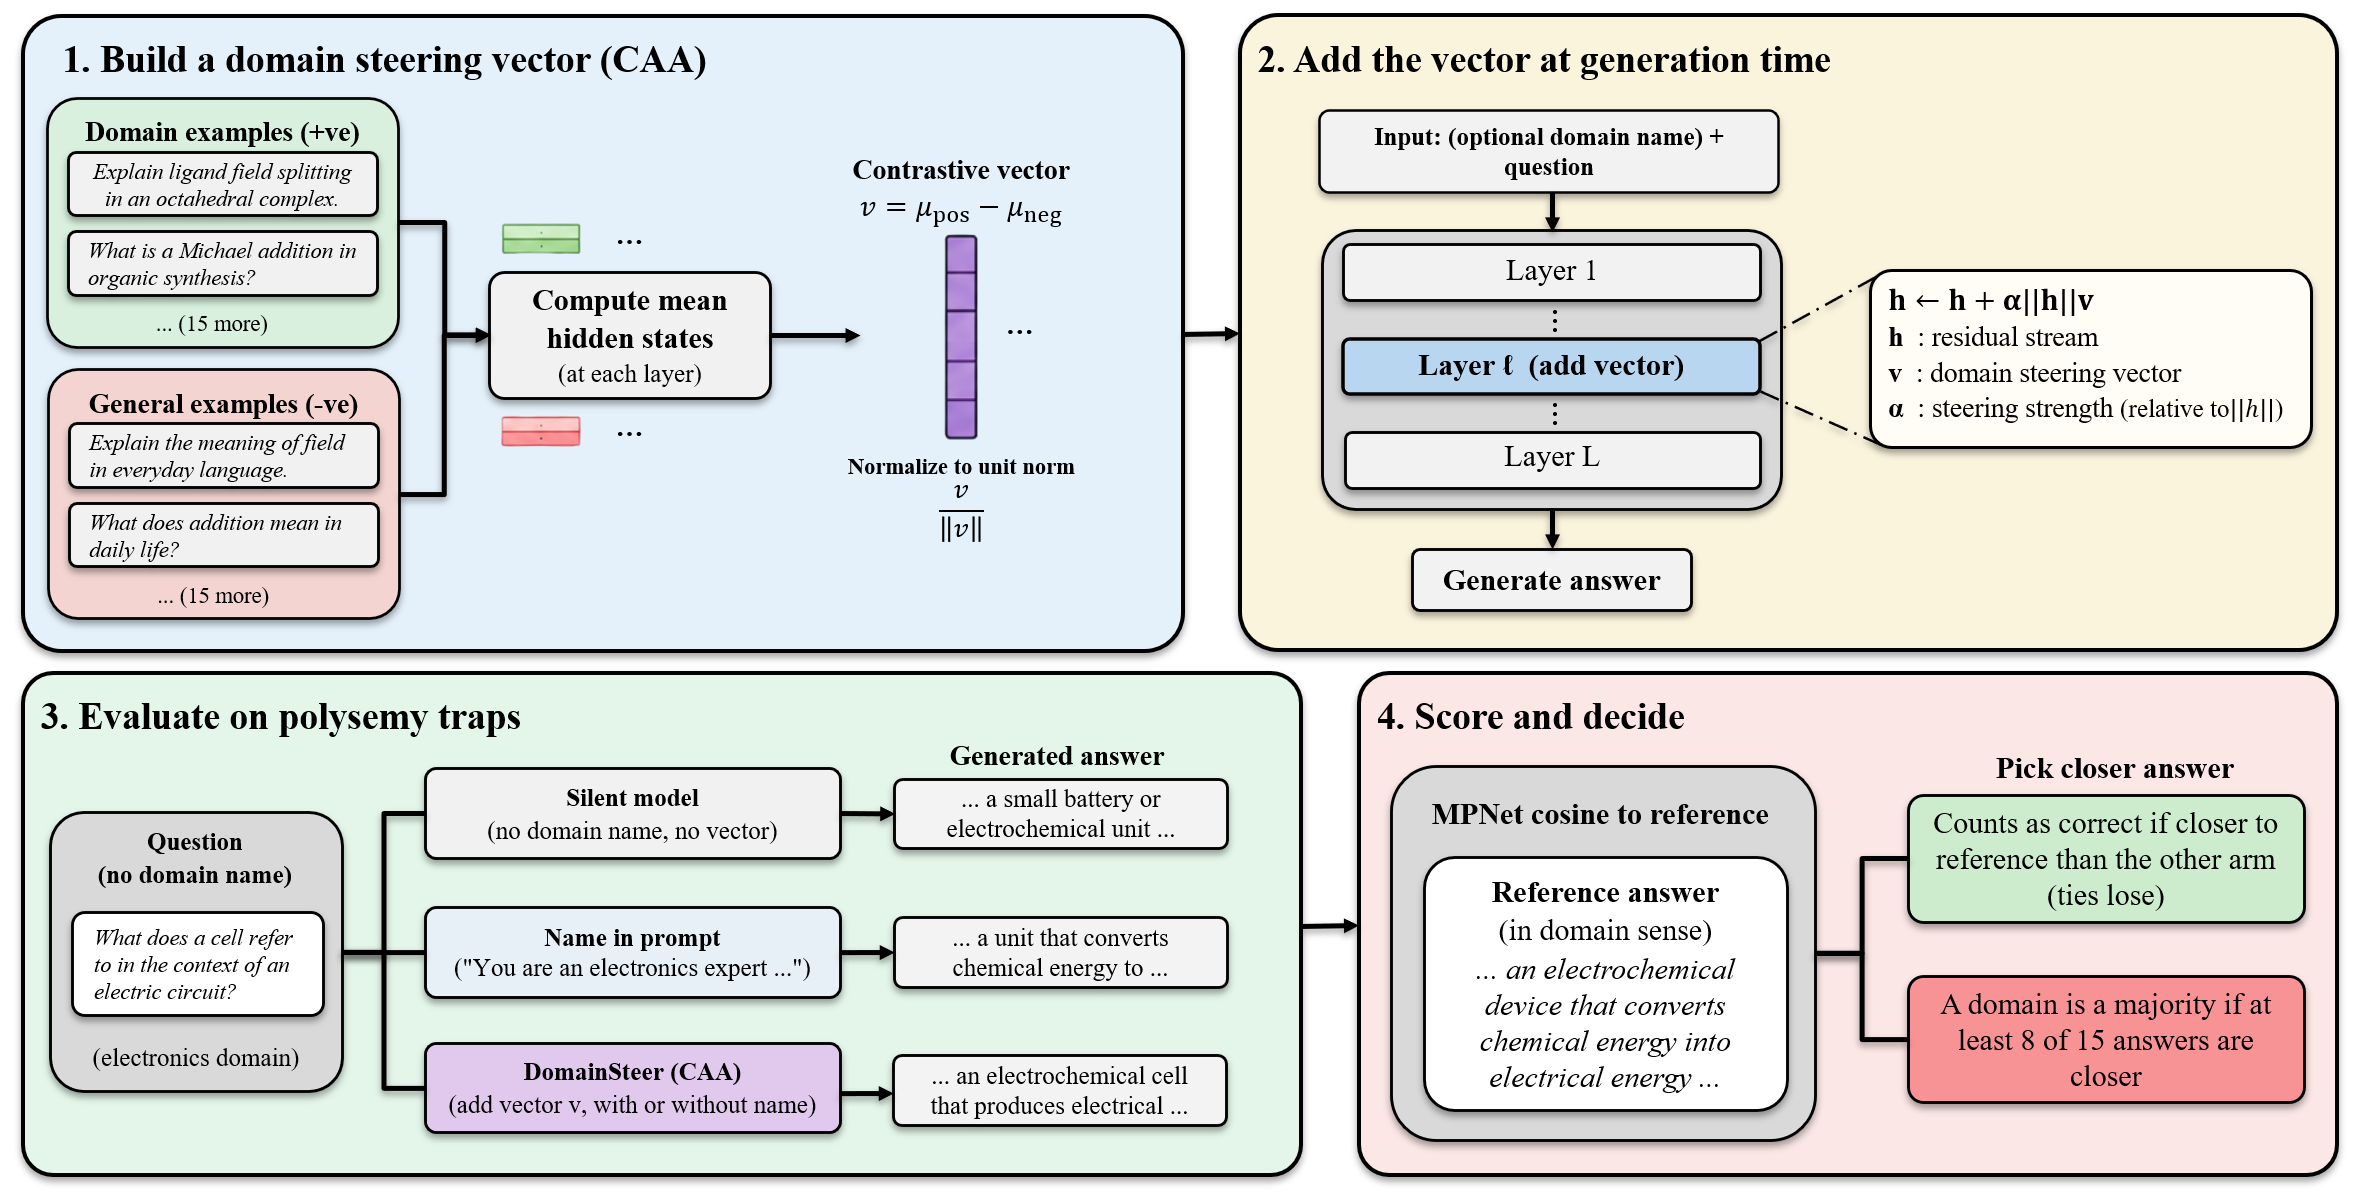
\includegraphics[width=\linewidth]{figures/fig_arch.png}
\end{center}
\caption{DomainSteer.
\textbf{(a)}~For each of 144 ANZSRC domains we collect 30 contrastive pairs: the same unnamed stems answered under a domain-committed system prompt (expert) and under a default helper prompt.
Assistant hidden states are mean-pooled at each middle layer; the steering vector is the unit difference of means.
Exam terms are held out of these pairs.
\textbf{(b)}~At generation time we add a norm-relative shift $h \leftarrow h + \alpha\|h\|v_\ell$ on one decoder-block output.
\textbf{(c)}~We ask 15 held-out polysemy traps per domain (2{,}160 items).
Four arms: unsteered, domain prompt, CAA, and prompt+CAA.
Each answer is ranked by MPNet cosine to one frozen gold.
We report the full $11\times 7$ layer--strength grid, not a single configuration.}
\label{fig:method}
\end{figure}

\subsection{Registry}

Targets are the 4-digit Fields of Research groups in ANZSRC 2020~\citep{anzsrc2020}.
That is the grain at which neighbouring fields start to collide: they reuse the same words with different operational readings.
A 2-digit division is still a broad umbrella; the 6-digit fields under a group are too uneven to use as domains (some groups have one restatement of the group name; others have a long list).
We keep \textbf{144} groups across all 22 divisions, from Agricultural, Veterinary and Food Sciences through Psychology, so agriculture, clinical medicine, electrical engineering, law, physics, and psychology sit in one registry.
Figure~\ref{fig:registry} is the map: five coarse umbrellas, 22 divisions, and the 144 groups underneath (not drawn).
Each group is one steerable domain.
Naming a group---\texttt{3106} or ``Industrial biotechnology''---is the user API.

\begin{figure}[h!]
\begin{center}
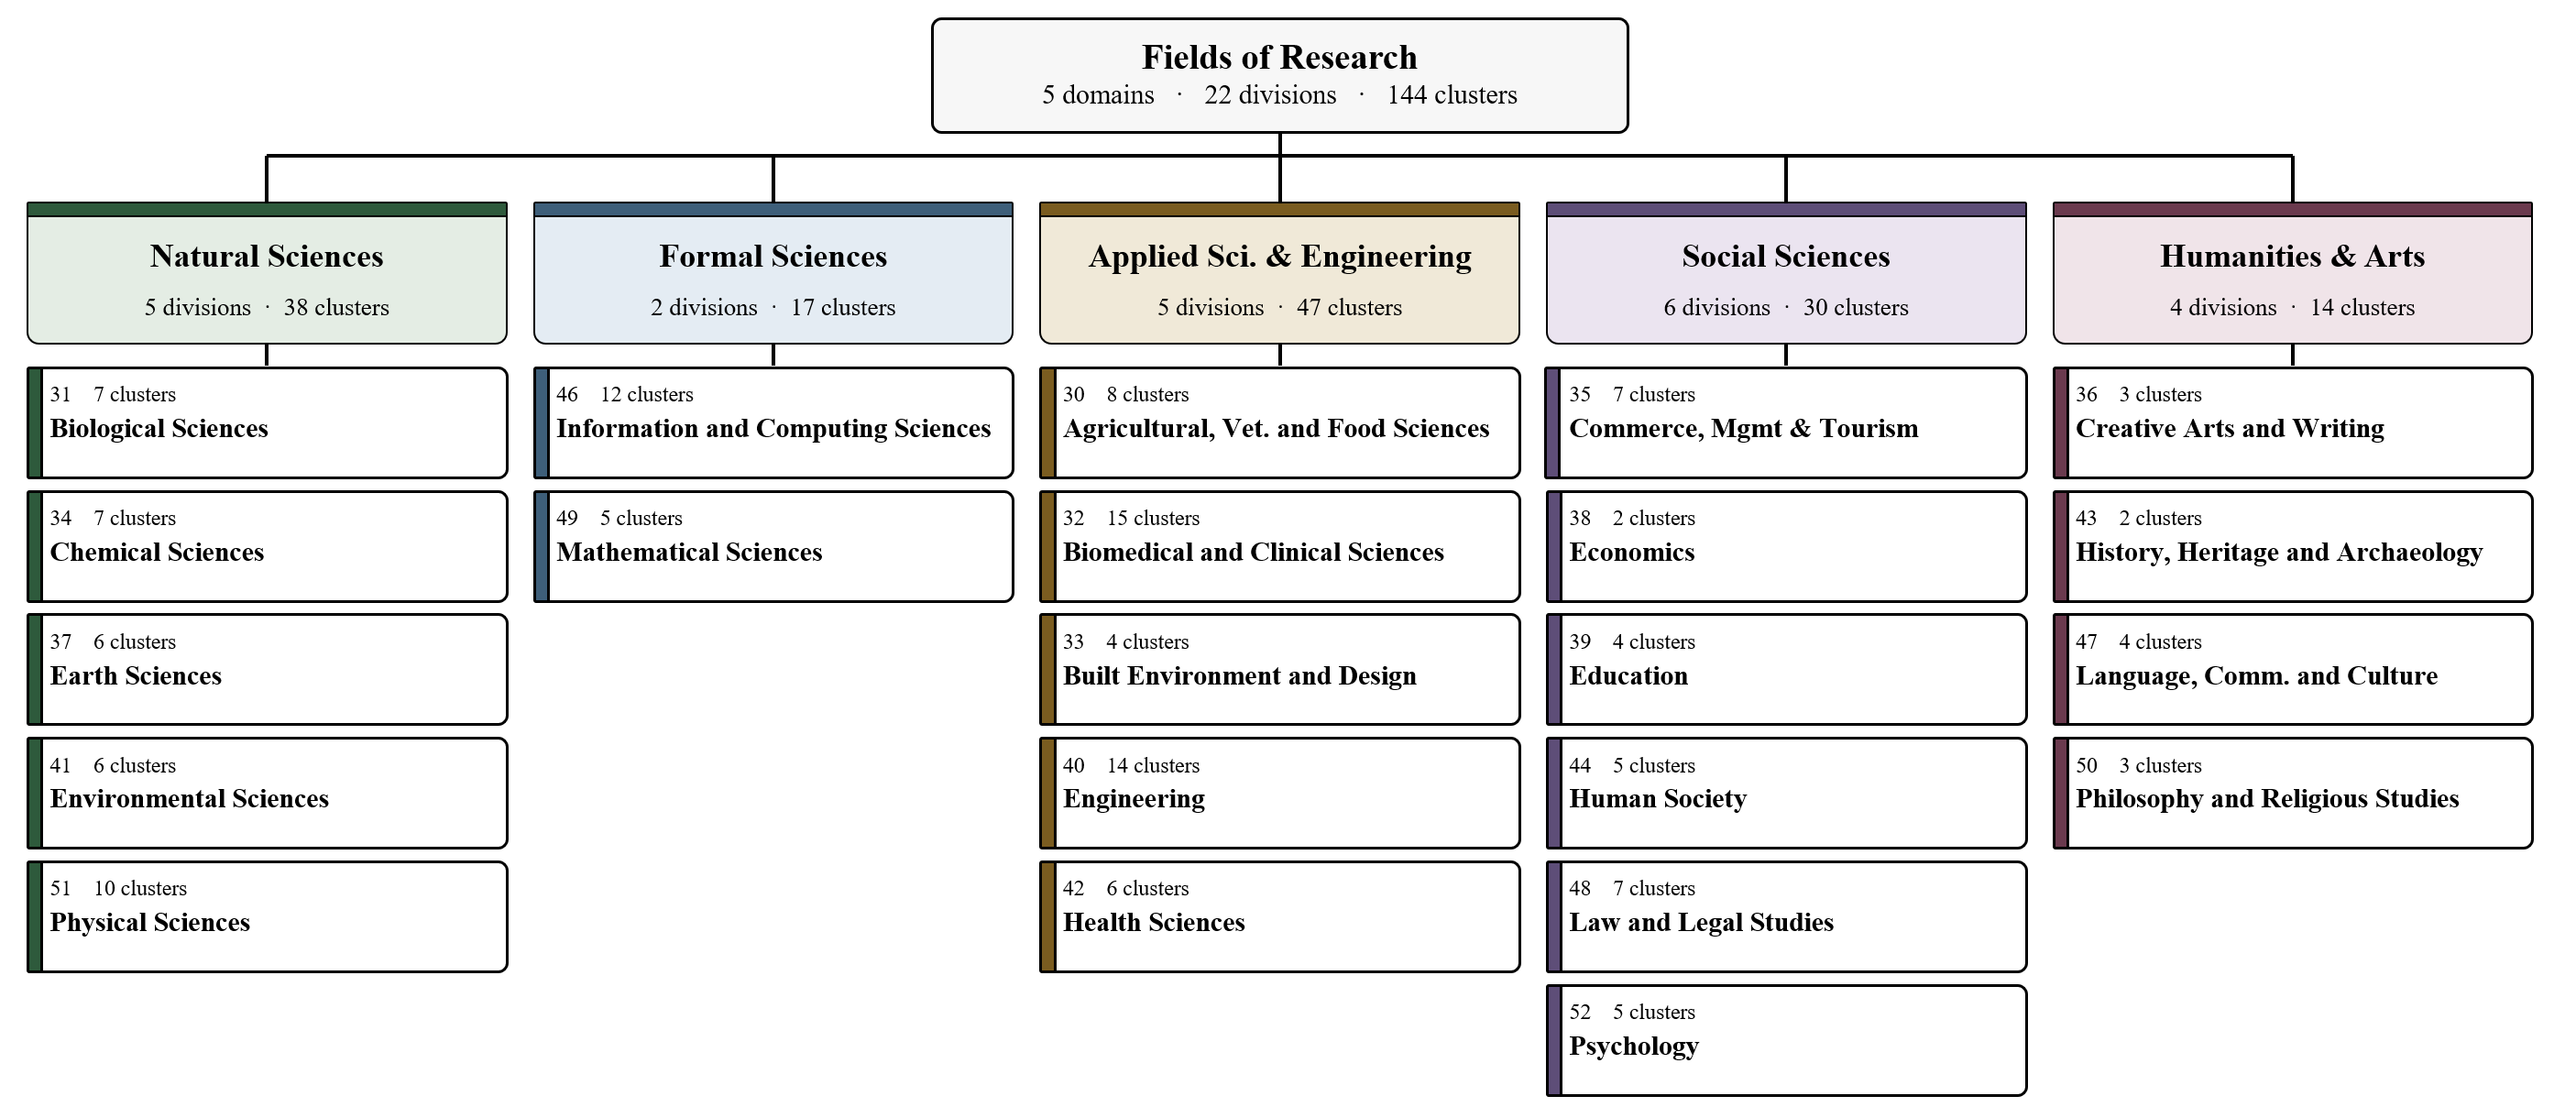
\includegraphics[width=\linewidth]{figures/fig_registry.png}
\end{center}
\caption{The DomainSteer registry (ANZSRC 2020).
Five umbrellas, 22 2-digit divisions, 144 4-digit groups (not drawn).
Each group is one steerable domain.
We use 4-digit groups because that is where neighbouring fields start to collide; 2-digit divisions are still broad, and 6-digit fields are too uneven to treat as domains.}
\label{fig:registry}
\end{figure}

Every domain is partitioned into \textbf{exactly ten} concept names (1{,}440 in total).
The names are globally disjoint: no concept key appears under two groups.
Uniform depth is the point.
We treat the 6-digit entries as seeds and generate ten sub-area names per group.
Pair generation is grounded in those names; the extracted vector is still a \emph{domain} direction, not a concept direction.
Appendix~\ref{app:registry} lists every group, its division, and those ten names.

\subsection{Contrastive pairs}

For each domain we collect \textbf{30} pairs.
The stems are unnamed: they do not contain the group title.
The same stem is answered twice by the model under test:
\begin{itemize}
\item \textbf{Expert $(+)$.} System prompt: the model is a practitioner of that domain and should give the field's operational reading of the term, including when the wording sounds like everyday life.
\item \textbf{Default $(-)$.} System prompt: ``You are a helpful assistant\ldots''---the same helper wrapper used later for unsteered and CAA generation.
\end{itemize}
The contrast identifier is \texttt{self\_gold\_expert\_vs\_default\_v1}.
Both sides are this model's own text.
Using 8B pairs to steer 3B (or the reverse) is not supported.

Exam terms are \textbf{held out} of these stems.
The polysemy-trap bank in \S\ref{sec:benchmark} records blocked terms per domain (for 3106: \emph{strain}, \emph{culture}, \emph{fingerprint}, \ldots).
Those words do not appear as pair stems, so $v$ is not fit on the test vocabulary.

\subsection{Extraction}

At extraction time both answers are replayed under the \textbf{same} chat template that generation uses: helper system prompt, unnamed stem, assistant span.
The domain-committed prompt is used only to \emph{write} the expert side; it is not present in the residual states we average.
Hidden states are mean-pooled over the assistant tokens at the output of decoder block $\ell$ (the same tensor a forward hook on that block will later modify).
For each layer
\begin{equation}
v_\ell = \mathrm{unit}(\mu_+ - \mu_-),
\end{equation}
the normalised difference of means~\citep{rimsky2024caa}.
We extract one unit vector at each of \textbf{layers 10--20} (11 vectors).
Linear separation of the two clouds on a concept-grouped holdout is recorded as a diagnostic; it is \emph{not} how this paper chooses a layer.
The paper reports every layer.

The library also implements an RFM estimator.
It is not used in the measurements below.

\subsection{Residual add}

At generation we register a forward hook on one decoder block and add a \textbf{norm-relative} shift to its output,
\begin{equation}
h \leftarrow h + \alpha \|h\| v_\ell,
\end{equation}
at every token position of that forward pass, including the system and user turns.
\citet{rimsky2024caa} typically add after the instruction; we do not.
$\alpha$ is a fraction of the residual norm at that position, so the same number is comparable across layers and tokens.
Decoding is greedy (\texttt{do\_sample=False}).
Unless noted, the hook stays on for the whole completion.

The user-facing \texttt{DomainSteerer} can pick a layer with an NLI judge and map a 0--1 \texttt{expertise} dial onto a calibrated $\alpha$.
Those defaults are for the API.
The measurements in \S\ref{sec:setup}--\ref{sec:results} do not use them: they sweep the full layer--strength grid.

\subsection{Polysemy-trap benchmark}
\label{sec:benchmark}

The exam is 144 domains $\times$ 15 items $=$ \textbf{2{,}160} questions.
A separate model (GPT-5.6-Terra) writes, for each domain, bare questions built around an overloaded term.
The question never names the field.
Each item records a \texttt{question} asked with no extra context; a short \texttt{gold} gloss of the domain sense (e.g.\ 3106 \emph{fingerprint} $\to$ product identity); a \texttt{baseline\_trap} everyday sense the unsteered model is expected to give (a person's identity); and one frozen reference sentence.

Every arm is scored against that sentence~\citep{song2020mpnet}, using \texttt{all-mpnet-base-v2}.
Scoring against a per-arm nearest paraphrase would be a different, easier measurement, and we do not do it.

This is a sense-selection test, not a knowledge benchmark.
A short answer that uses the domain reading of \emph{fingerprint} is closer to the frozen gold than one that uses the biometric reading; that is all the score claims.

\section{Experimental setup}
\label{sec:setup}

We report three grids, all layers $10$--$20$ $\times$ $\alpha \in \{0.10, 0.15, 0.20, 0.25, 0.30, 0.35, 0.40\}$ (77 cells), greedy decoding.
They are not one experiment: the length cap and the arms differ, and we do not pool the majority counts.

\begin{itemize}
\item \textbf{8B, 10-word CAA grid.} Llama-3.1-8B-Instruct, $\leq 10$ words / one sentence (16 new tokens, then clip). Unsteered, domain prompt, and CAA. CAA versus the name: \textbf{113/144}.
\item \textbf{8B, 20-word four-arm grid.} The same model, $\leq 20$ words / two sentences (40 new tokens, then clip). Adds prompt+CAA. All three comparisons: CAA versus silent \textbf{144/144}, CAA versus the name \textbf{103/144}, prompt+CAA versus prompt \textbf{141/144}.
\item \textbf{3B, 10-word four-arm grid.} Llama-3.2-3B-Instruct, $\leq 10$ words / one sentence. The same three comparisons: \textbf{144/144}, \textbf{131/144}, \textbf{139/144}. A replication of the qualitative pattern, not a size comparison with either 8B cap.
\end{itemize}

\begin{table}[t]
\caption{Four arms. The domain prompt names the ANZSRC group in the system message and does not name it in the user question.}
\label{tab:arms}
\begin{center}
\small
\begin{tabular}{lll}
\toprule
\textbf{Arm} & \textbf{System prompt} & \textbf{Vector} \\
\midrule
unsteered & helper, no domain & off \\
prompt & ``You are a \{domain\} practitioner'' & off \\
CAA & helper & on \\
prompt+CAA & domain prompt & on \\
\bottomrule
\end{tabular}
\end{center}
\end{table}

Table~\ref{tab:arms} is the $2\times 2$.
Both system prompts end with the length cap for that run (``Answer in at most 10 words'' or ``20 words. Do not use lists.'').
The exact templates, including the pair-writing expert prompt, are in Appendix~\ref{app:prompts}.
Unsteered and prompt are generated once per item; the steered arms are generated at every cell.

\paragraph{Score.}
Let $\mathrm{sim}$ be the cosine between \texttt{all-mpnet-base-v2} embeddings of the answer and of that item's frozen gold~\citep{reimers2019sbert,song2020mpnet}.
An item win for arm $A$ over arm $B$ is $\mathrm{sim}_A > \mathrm{sim}_B$ (ties lose).
A domain majority is at least 8 item wins out of 15.

\paragraph{Per-domain best is an envelope.}
For each domain we pick the cell with the most item wins against the stated reference arm, breaking ties by higher mean gold cosine.
That cell is chosen on the same 15 items it is then scored on, so the 144 / 103 / 141 and 113/144 counts are an \emph{upper bound} on this vector and this exam, not a deployment recipe.
We always place next to them (i)~mean item-win counts, not only the $\geq 8$ cut, and (ii)~the number of domains in majority at \emph{every} cell of the grid, with no per-domain selection.

\section{Results}
\label{sec:results}

Table~\ref{tab:headline} is the headline.
Figure~\ref{fig:wins} is the corresponding win-count histogram on 8B.
Naming the domain already moves mean gold cosine from $0.341$ (silent, 20-word) to $0.495$, and from $0.355$ to $0.488$ on the 10-word 8B grid.
The question is whether $v$ adds anything beyond that, and whether it can replace it.

\begin{table}[t]
\caption{Per-domain best of 77 cells.
A domain counts if $\geq 8/15$ answers are strictly closer to the frozen gold than the reference arm.
The 8B 10-word grid has no prompt+CAA arm; the 8B 20-word and 3B grids are four-arm.
Do not read a row as a model-size effect.}
\label{tab:headline}
\begin{center}
\small
\begin{tabular}{llccccc}
\toprule
 &  & mean sim & mean sim & \multicolumn{3}{c}{domains with majority} \\
\cmidrule(lr){5-7}
Model & cap & silent & prompt & CAA vs silent & CAA vs prompt & prompt+CAA vs prompt \\
\midrule
Llama-3.1-8B & $\leq 10$ w / 1 sent. & 0.355 & 0.488 & --- & 113/144 & --- \\
 & & & & & (9.03) & \\
Llama-3.1-8B & $\leq 20$ w / 2 sent. & 0.341 & 0.495 & 144/144 & 103/144 & 141/144 \\
 & & & & (14.19) & (8.78) & (10.88) \\
Llama-3.2-3B & $\leq 10$ w / 1 sent. & 0.345 & 0.443 & 144/144 & 131/144 & 139/144 \\
 & & & & (13.22) & (9.81) & (10.90) \\
\bottomrule
\end{tabular}
\end{center}
\vspace{-0.4em}
{\small Parentheses: mean item wins / 15 at that domain's best cell.}
\end{table}

\begin{figure}[t]
\begin{center}
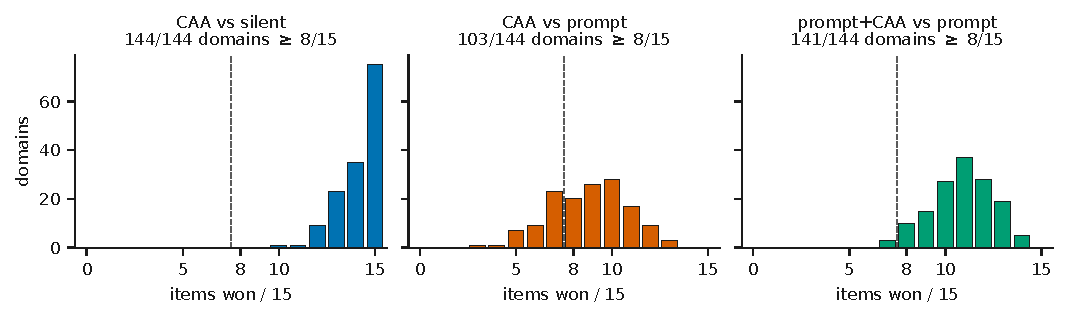
\includegraphics[width=\linewidth]{figures/fig_wins.pdf}
\end{center}
\caption{Llama-3.1-8B-Instruct, 20-word four-arm grid.
Distribution of per-domain item wins at the best of 77 cells.
Dashed line: majority cut ($\geq 8/15$).
CAA vs.\ silent is saturated; CAA vs.\ the name is the mixed arm; adding $v$ on top of the name is the reliable extra.}
\label{fig:wins}
\end{figure}

\subsection{CAA versus the silent model}

At each domain's best cell on the 20-word four-arm grid, CAA places a majority of answers closer to gold than the silent helper in \textbf{144/144} domains (mean 14.19/15; 75 domains win all 15).
Mean gold cosine at those cells is $0.491$, against $0.341$ silent.
The vector, used without naming the field, is enough to beat the everyday prior on this exam.
That is the easy comparison.

\subsection{CAA versus naming the domain}

Against the domain prompt, the 20-word four-arm grid gives \textbf{103/144} domains (mean 8.78/15; mean cosine $0.493$).
Forty-one domains stay at 7/15 or below (worst: fisheries sciences 3/15; microbiology 4/15).
The 10-word CAA grid, the same model and exam with a shorter cap and no prompt+CAA arm, gives \textbf{113/144} (mean 9.03/15; mean cosine $0.489$ against the prompt's $0.488$).
The prompt is not a straw man~\citep{zheng2024personas,wu2025axbench}: it is already a strong sense selector, and a residual-stream copy of the same contrast only sometimes outranks restating the name on held-out words.
We do not pool 103 and 113.

\subsection{Adding the vector on top of the name}

Prompt+CAA versus prompt, on the 20-word four-arm grid, is the comparison that holds: \textbf{141/144} domains (mean 10.88/15; mean cosine $0.529$).
The three misses are 7/15 each (cardiovascular medicine and haematology; traditional, complementary and integrative medicine; classical physics).
The two interventions are not substitutes.
The name does much of the work; $v$ is a reliable increment on top of it.

Table~\ref{tab:qual} shows one item from industrial biotechnology (3106).
Both the silent model and the domain prompt give the biometric reading of \emph{fingerprint}.
CAA and prompt+CAA move toward a product/strain reading.
Cosine can rank that shift without the answer matching the gold sentence word for word; we do not claim more than the ranking.
Appendix~\ref{app:responses} lists one best-cell example per domain.

\begin{table}[t]
\caption{One trap (industrial biotechnology, 3106). Gold is the frozen reference.
CAA cell $(10,0.25)$; prompt+CAA cell $(11,0.15)$; 20-word four-arm grid.}
\label{tab:qual}
\begin{center}
\small
\begin{tabular}{p{0.22\linewidth}p{0.52\linewidth}r}
\toprule
Arm & Answer (clipped) & sim \\
\midrule
gold & It separates closely related fermentation products by their chemical signatures. & --- \\
unsteered & A fingerprint can distinguish one individual from another due to unique ridge patterns. & 0.33 \\
prompt & A fingerprint can distinguish one individual from another, even among identical twins. & 0.30 \\
CAA & A fingerprint can distinguish between different strains of bacteria. & 0.52 \\
prompt+CAA & A fingerprint can distinguish an individual organism \ldots strain identification in bioprocess development. & 0.52 \\
\bottomrule
\end{tabular}
\end{center}
\end{table}

\subsection{Strength and layer are not shared}

Figure~\ref{fig:settings} shows each domain's best $\alpha$ and best layer under the two comparisons against the prompt, both on the 20-word four-arm grid.
CAA-alone cells concentrate at higher $\alpha$ (mostly $0.25$--$0.40$).
Prompt+CAA cells concentrate at lower $\alpha$ (mostly $0.10$--$0.20$).
Best layers cover the whole $10$--$20$ range in both arms (39 distinct cells for CAA vs.\ prompt; 54 for prompt+CAA).
There is no ``steer at layer 16, $\alpha=0.3$'' recipe.

\begin{figure}[t]
\begin{center}
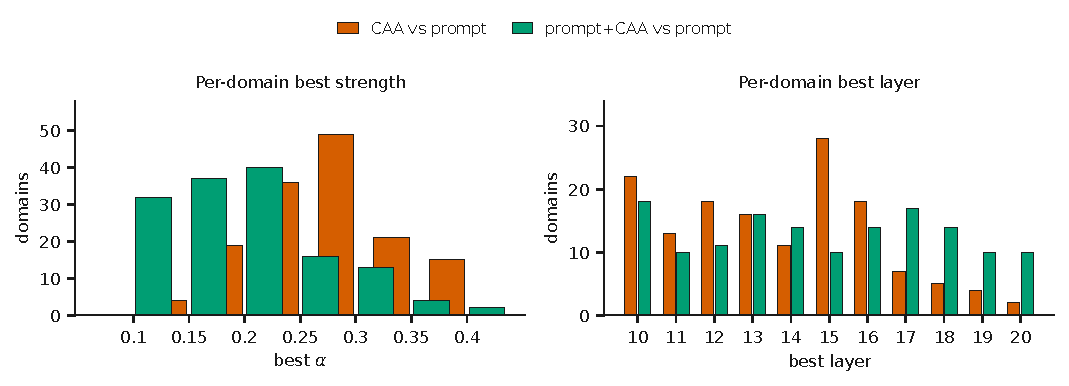
\includegraphics[width=\linewidth]{figures/fig_settings.pdf}
\end{center}
\caption{Llama-3.1-8B-Instruct, 20-word four-arm grid.
Histogram of the per-domain best $\alpha$ (left) and best layer (right) for CAA vs.\ prompt and prompt+CAA vs.\ prompt.
Useful strength is higher when the prompt is silent, lower when the domain is already named.
Best layer is not concentrated.}
\label{fig:settings}
\end{figure}

\subsection{The grid, with no per-domain selection}

Figure~\ref{fig:grid} asks a different question: at a \emph{fixed} $(L,\alpha)$, in how many domains does that one cell already have a majority of item wins?
On the 8B four-arm grid the peaks are \textbf{144/144} for CAA vs.\ silent (layer 15, $\alpha=0.25$), \textbf{47/144} for CAA vs.\ prompt (layer 10, $\alpha=0.25$), and \textbf{99/144} for prompt+CAA vs.\ prompt (layer 13, $\alpha=0.10$).
On 3B they are 138, 69, and 97.
The 10-word 8B CAA-vs-prompt heatmap, in the appendix (Figure~\ref{fig:grid-10w}), peaks at 59/144 (layer 15, $\alpha=0.35$).
Every shared-cell peak trails the corresponding per-domain envelope.
A shared setting is a real intervention; it is not what the oracle counts describe.
That is why we report the grid.

\begin{figure}[t]
\begin{center}
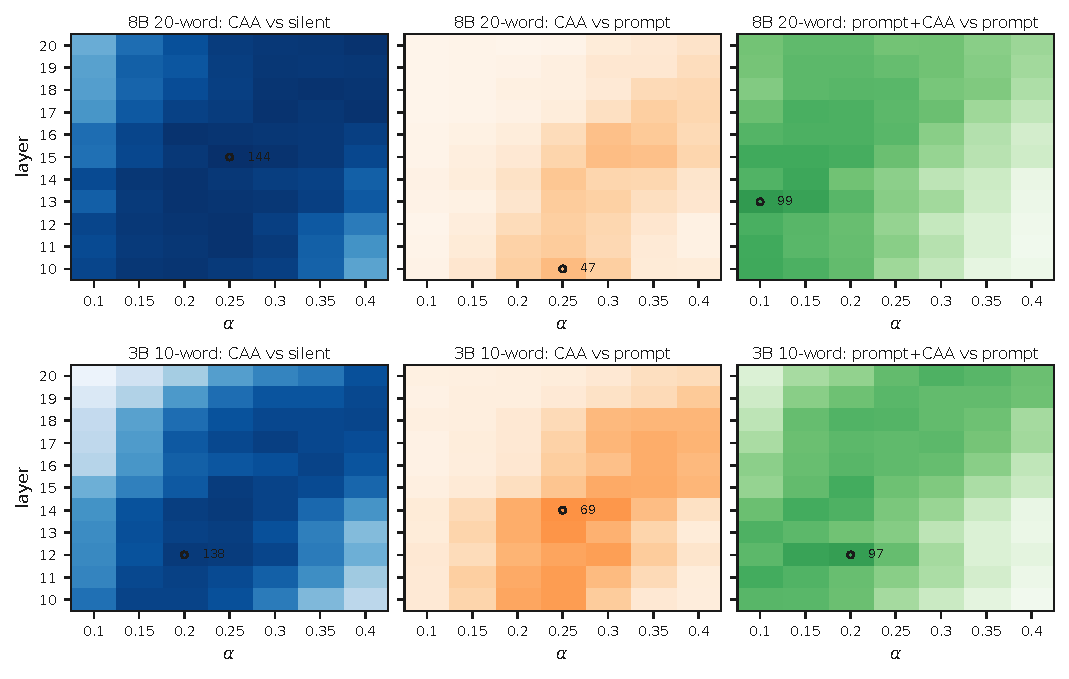
\includegraphics[width=\linewidth]{figures/fig_grid.pdf}
\end{center}
\caption{Domains with $\geq 8/15$ item wins at each of the 77 cells, with no per-domain selection.
Top: Llama-3.1-8B-Instruct, 20-word four-arm.
Bottom: Llama-3.2-3B-Instruct, 10-word four-arm.
Circled cell: the maximum.
8B peaks: 144 (CAA vs.\ silent), 47 (CAA vs.\ prompt), 99 (prompt+CAA vs.\ prompt).
3B peaks: 138, 69, 97.}
\label{fig:grid}
\end{figure}

\subsection{Llama-3.2-3B}

On Llama-3.2-3B-Instruct, with a 10-word / one-sentence cap and the same 77-cell four-arm grid, the per-domain best cell gives CAA vs.\ silent \textbf{144/144} (mean 13.22/15), CAA vs.\ prompt \textbf{131/144} (mean 9.81), and prompt+CAA vs.\ prompt \textbf{139/144} (mean 10.90).
Silent and prompt mean cosines are $0.345$ and $0.443$.
Figure~\ref{fig:grid} (bottom) is the corresponding shared-cell heatmap.
The qualitative picture is the same: $v$ always beats silence; $v$ versus the name is the mixed arm; name+$v$ is the reliable extra; best layer and $\alpha$ again cover the whole grid.
Because the length cap differs, we do not treat 131 vs.\ 103 or 113 as a size effect.

\section{Limitations}

The main grid is one model family (Llama-3.1-8B-Instruct) and 15 items per domain; $\geq 8/15$ is a noisy majority, which is why we show the full win-count histogram.
The 8B CAA-versus-name counts (113 on the 10-word grid, 103 on the 20-word four-arm grid) and the 8B stacking count (141) come from two grids with different length caps; we do not pool them.
The per-domain best of 77 is an upper bound on those same 15 items.
Gold questions and the frozen gold sentence are GPT-written; cosine to that sentence is not a human expertise rating, and it can rank a format-matched paraphrase that has not actually changed sense.
Answers are short (20 words on the 8B four-arm, 10 on the 8B CAA grid and on 3B): the test is sense selection, not long-form scientific writing.
The vector comes from this model's own domain-prompt vs.\ default completions, so CAA is in part a residual-stream copy of that prompt contrast.
That makes 103/144 and 113/144 more interesting, not less: the activation version only sometimes outranks restating the name on held-out words.
We do not evaluate side effects on unrelated queries~\citep{stickland2024kts}, multi-domain composition~\citep{vanderweij2024extending}, or transfer of $v$ across model families.

\section{Conclusion}

We released DomainSteer: CAA for 144 scientific domains, with contrastive pairs for two Llama Instruct models and a 2{,}160-item polysemy-trap exam scored against one frozen gold per item.
On Llama-3.1-8B-Instruct, at each domain's best of 77 layer--strength cells, the 20-word four-arm grid gives CAA over silent in 144/144 domains, CAA over the name in 103/144, and prompt+CAA over the name in 141/144; the 10-word CAA grid gives 113/144 against the name.
The cell that produces those counts is not shared, so the measurement we stand behind is the grid.

\subsubsection*{AI use statement}

----

\subsubsection*{Ethics statement}

----

\subsubsection*{Reproducibility statement}

The DomainSteer library, the 144-domain registry, 4{,}320 contrastive pairs per shipped model, and the 2{,}160-item exam ship as package data.
Section~\ref{sec:setup} specifies the four arms, the $11\times 7$ grid, greedy decoding, the 10-word and 20-word caps, the MPNet scoring model, the item-win rule, and the majority cut.
An anonymous code and data archive is included as supplementary material.

\bibliography{iclr2027_conference}
\bibliographystyle{iclr2027_conference}

\appendix
\section{Prompts}
\label{app:prompts}

The user turn is always the bare question. Nothing below is inserted into
the question text.

\subsection{Contrastive pairs}

The same unnamed stem is answered twice by the model under test. Expert
text is the positive class; default text is the negative class.
Extraction replays both answers under the default helper template.

\paragraph{Expert $(+)$.}
\begin{quote}\small\ttfamily\raggedright
You are a \{domain\} practitioner. Every question uses a term that has an
operational meaning in \{domain\}. Answer that meaning even when the wording
sounds like everyday life, media, sports, law, or another field --- those
readings are distractors, not the answer. Answer in 1-2 short sentences.
Do not use lists. Do not explain other fields' meanings of the term.
\end{quote}

\paragraph{Default $(-)$, and extraction wrapper.}
\begin{quote}\small\ttfamily\raggedright
You are a helpful assistant. Answer in 1-2 short sentences. Do not use lists.
\end{quote}

\subsection{Evaluation arms}

Unsteered and CAA use the helper prompt (no domain name). Prompt and
prompt+CAA use the practitioner prompt. The length cap matches the run.

\paragraph{Helper (unsteered, CAA), 10-word runs.}
\begin{quote}\small\ttfamily\raggedright
You are a helpful assistant. Answer in at most 10 words. Do not use lists.
\end{quote}

\paragraph{Practitioner (prompt, prompt+CAA), 10-word runs.}
\begin{quote}\small\ttfamily\raggedright
You are a \{domain\} practitioner. Answer in at most 10 words. Do not use lists.
\end{quote}

\paragraph{Helper, 20-word four-arm run.}
\begin{quote}\small\ttfamily\raggedright
You are a helpful assistant. Answer in at most 20 words. Do not use lists.
\end{quote}

\paragraph{Practitioner, 20-word four-arm run.}
\begin{quote}\small\ttfamily\raggedright
You are a \{domain\} practitioner. Answer in at most 20 words. Do not use lists.
\end{quote}

\section{Best-cell responses (8B, 20-word four-arm)}
\label{app:responses}

One item per domain: the trap with the largest prompt+CAA vs.\ prompt
cosine gain at that domain's best prompt+CAA cell.
Cosines in parentheses are MPNet similarity to the frozen gold.
CAA and prompt+CAA answers are from that arm's own best cell, which need
not be the same $(L,\alpha)$.

\begingroup\small
\medskip\noindent\textbf{3001 Agricultural biotechnology.} Term: \emph{draft}.
Q: What can a draft describe?
\begin{itemize}\setlength{\itemsep}{0.15em}\setlength{\parsep}{0pt}\setlength{\topsep}{0.2em}
\item Gold: It can describe a preliminary genome sequence assembly.
\item Unsteered (0.34): A draft can describe a preliminary version of a document, a current of air, or a selection of players in
\item Prompt (0.19): A draft in agriculture refers to a controlled environment with a gentle flow of air, often used in greenhouses or
\item CAA $L16$, $\alpha=0.35$ (0.51): A draft is a gene expression vector used in biotechnology to produce a desired trait in plants.
\item Prompt+CAA $L13$, $\alpha=0.2$ (0.53): A draft in biotechnology refers to the process of introducing a gene from one species into another species using biotechnology
\end{itemize}
\medskip\noindent\textbf{3002 Agriculture, land and farm management.} Term: \emph{draft}.
Q: What does draft quantify?
\begin{itemize}\setlength{\itemsep}{0.15em}\setlength{\parsep}{0pt}\setlength{\topsep}{0.2em}
\item Gold: It measures implement pulling resistance through the soil.
\item Unsteered (0.26): A draft quantifies the amount of air or gas that passes through a system or device per unit of time.
\item Prompt (0.27): Draft refers to the amount of feed required to maintain a certain level of weight gain or production in livestock
\item CAA $L15$, $\alpha=0.35$ (0.51): Draft quantifies crop yields, soil health, and crop growth through measurements of plant growth and crop yields.
\item Prompt+CAA $L14$, $\alpha=0.2$ (0.40): Draft is the amount of water lost through evaporation from soil surface, measured in inches or centimeters.
\end{itemize}
\medskip\noindent\textbf{3003 Animal production.} Term: \emph{dam}.
Q: What does a dam identify?
\begin{itemize}\setlength{\itemsep}{0.15em}\setlength{\parsep}{0pt}\setlength{\topsep}{0.2em}
\item Gold: It indicates the female ancestor listed as the mother.
\item Unsteered (0.18): A dam identifies a barrier constructed across a river or stream to control water flow and water level.
\item Prompt (0.14): A dam identifies a barrier constructed across a watercourse to control water flow, typically for irrigation, power generation, or flood
\item CAA $L15$, $\alpha=0.35$ (0.46): A dam identifies the sire of a female livestock, used in breeding programs to improve genetic traits.
\item Prompt+CAA $L18$, $\alpha=0.1$ (0.46): A dam identifies the female parent of an animal, especially in cattle, sheep, and other livestock breeding programs.
\end{itemize}
\medskip\noindent\textbf{3004 Crop and pasture production.} Term: \emph{sink}.
Q: What does a sink receive?
\begin{itemize}\setlength{\itemsep}{0.15em}\setlength{\parsep}{0pt}\setlength{\topsep}{0.2em}
\item Gold: It receives sucrose transported through the phloem.
\item Unsteered (0.27): A sink receives water, typically from a faucet or water supply line, for washing and draining purposes.
\item Prompt (0.29): A sink receives water, typically from a faucet or pipe, to be used for various purposes such as washing or
\item CAA $L17$, $\alpha=0.4$ (0.61): A sink receives water, nutrients, and crop residues from the crop roots through the root crown.
\item Prompt+CAA $L20$, $\alpha=0.25$ (0.46): A sink receives water, nutrients, and organic matter from crop and pasture residues, and excess water from rainfall.
\end{itemize}
\medskip\noindent\textbf{3005 Fisheries sciences.} Term: \emph{cleaner}.
Q: What can a cleaner remove?
\begin{itemize}\setlength{\itemsep}{0.15em}\setlength{\parsep}{0pt}\setlength{\topsep}{0.2em}
\item Gold: It can remove ectoparasitic lice from cultured salmon.
\item Unsteered (0.26): A cleaner can remove dirt, dust, stains, grime, grease, and other impurities from surfaces and objects.
\item Prompt (0.56): A cleaner fish can remove parasites, dead skin, and other debris from the bodies of other fish.
\item CAA $L19$, $\alpha=0.4$ (0.46): A cleaner can remove a variety of substances including algae, grime, and marine life from fishing gear.
\item Prompt+CAA $L19$, $\alpha=0.2$ (0.65): A cleaner wrasse can remove parasitic fish, such as sea lice, from the skin of other fish.
\end{itemize}
\medskip\noindent\textbf{3007 Forestry sciences.} Term: \emph{figure}.
Q: What does figure describe?
\begin{itemize}\setlength{\itemsep}{0.15em}\setlength{\parsep}{0pt}\setlength{\topsep}{0.2em}
\item Gold: It describes the decorative pattern visible in wood grain.
\item Unsteered (0.26): A figure is a representation of a person, animal, or object in art, often two-dimensional or three-dimensional.
\item Prompt (0.14): I'm not sure what you're referring to, could you please provide more context or clarify what you mean by "figure"?
\item CAA $L10$, $\alpha=0.25$ (0.43): Figure describes a woody vegetation stand dominated by trees of similar age and species, often with uniform canopy density.
\item Prompt+CAA $L13$, $\alpha=0.15$ (0.43): A figure in forestry refers to a tree with a straight, columnar shape, typically with a single stem and a
\end{itemize}
\medskip\noindent\textbf{3008 Horticultural production.} Term: \emph{load}.
Q: What can load determine?
\begin{itemize}\setlength{\itemsep}{0.15em}\setlength{\parsep}{0pt}\setlength{\topsep}{0.2em}
\item Gold: It influences berry calibre at harvest.
\item Unsteered (0.15): A load can determine weight, mass, or capacity, often used in physics, engineering, and construction to measure various types of
\item Prompt (0.23): Load can determine the structural integrity of a greenhouse, affecting its stability and potential for collapse under weight.
\item CAA $L11$, $\alpha=0.2$ (0.39): Load can determine plant growth, soil moisture, and nutrient availability in agricultural settings.
\item Prompt+CAA $L14$, $\alpha=0.2$ (0.52): Load can determine plant growth, yield, and fruiting in horticulture, as it affects nutrient availability and root development.
\end{itemize}
\medskip\noindent\textbf{3009 Veterinary sciences.} Term: \emph{ring}.
Q: What can a ring indicate?
\begin{itemize}\setlength{\itemsep}{0.15em}\setlength{\parsep}{0pt}\setlength{\topsep}{0.2em}
\item Gold: It can indicate dermatophytosis caused by a dermatophyte infection.
\item Unsteered (0.16): A ring can indicate a commitment, engagement, marriage, or a symbol of status, power, or wealth in various cultures.
\item Prompt (0.23): A ring on a bird's leg can indicate that it has been banded for identification or tracking purposes.
\item CAA $L14$, $\alpha=0.35$ (0.26): A ring can indicate a marriage in dogs, a marking in a male bovine, or an esophageal esophitis in a
\item Prompt+CAA $L13$, $\alpha=0.15$ (0.45): A ring on the nail can indicate a foreign body, such as a grass awn, in the hoof.
\end{itemize}
\medskip\noindent\textbf{3101 Biochemistry and cell biology.} Term: \emph{resolution}.
Q: What can resolution distinguish?
\begin{itemize}\setlength{\itemsep}{0.15em}\setlength{\parsep}{0pt}\setlength{\topsep}{0.2em}
\item Gold: Resolution can distinguish protein isoforms that differ slightly in mass or charge.
\item Unsteered (0.44): Resolution can distinguish between two closely related or similar objects, images, or signals.
\item Prompt (0.49): Resolution in microscopy can distinguish objects or structures as small as 200-300 nanometers apart, depending on the technique used.
\item CAA $L17$, $\alpha=0.35$ (0.74): Resolution can distinguish between two proteins, two proteins and a protein complex, and two protein complexes.
\item Prompt+CAA $L19$, $\alpha=0.2$ (0.78): Resolution in biochemistry and cell biology can distinguish between two or more molecules, proteins, or structures based on their size
\end{itemize}
\medskip\noindent\textbf{3102 Bioinformatics and computational biology.} Term: \emph{browser}.
Q: What can a browser navigate?
\begin{itemize}\setlength{\itemsep}{0.15em}\setlength{\parsep}{0pt}\setlength{\topsep}{0.2em}
\item Gold: A genome browser can navigate genomic coordinates across a reference assembly.
\item Unsteered (0.32): A browser can navigate the internet, websites, web pages, and online applications.
\item Prompt (0.30): A web browser can navigate through the World Wide Web, accessing various websites, web pages, and online resources.
\item CAA $L11$, $\alpha=0.25$ (0.79): A browser can navigate a genome assembly, a genome assembly graph, or a genome assembly graph with a graph library.
\item Prompt+CAA $L17$, $\alpha=0.2$ (0.68): A browser can navigate through genomic sequences, transcriptomes, and proteomes to identify functional regions and predict gene function.
\end{itemize}
\medskip\noindent\textbf{3104 Evolutionary biology.} Term: \emph{signal}.
Q: What does signal reveal?
\begin{itemize}\setlength{\itemsep}{0.15em}\setlength{\parsep}{0pt}\setlength{\topsep}{0.2em}
\item Gold: It reveals shared ancestry among the taxa.
\item Unsteered (0.17): A signal can reveal information, convey meaning, or indicate a change in a system, process, or situation.
\item Prompt (0.13): Signal transduction pathways reveal how cells respond to environmental cues, influencing gene expression and cellular behavior through complex molecular interactions.
\item CAA $L10$, $\alpha=0.25$ (0.52): Signal reveals the genetic basis of a trait, its evolutionary history, and its ecological niche.
\item Prompt+CAA $L17$, $\alpha=0.35$ (0.42): A signal in the context of evolutionary biology is a heritable trait that provides a genetic advantage to a species.
\end{itemize}
\medskip\noindent\textbf{3106 Industrial biotechnology.} Term: \emph{bed}.
Q: What can a bed support?
\begin{itemize}\setlength{\itemsep}{0.15em}\setlength{\parsep}{0pt}\setlength{\topsep}{0.2em}
\item Gold: The bed supports a retained biocatalyst.
\item Unsteered (0.45): A bed can support a person's body weight, providing a comfortable place to sleep and rest.
\item Prompt (0.45): A bed can support a person's body weight, providing a comfortable surface for rest and relaxation.
\item CAA $L10$, $\alpha=0.25$ (0.63): A bioreactor bed supports the growth of microorganisms for biofuel production and production of recombinant proteins.
\item Prompt+CAA $L11$, $\alpha=0.15$ (0.69): A bioreactor bed can support microbial fermentation for the production of biofuels, biochemicals, and bioproducts.
\end{itemize}
\medskip\noindent\textbf{3107 Microbiology.} Term: \emph{fingerprint}.
Q: What can a fingerprint distinguish?
\begin{itemize}\setlength{\itemsep}{0.15em}\setlength{\parsep}{0pt}\setlength{\topsep}{0.2em}
\item Gold: It separates strains within the same species.
\item Unsteered (0.28): A fingerprint can distinguish one individual from another due to unique patterns and ridges on an individual's fingertips.
\item Prompt (0.27): A fingerprint can distinguish one individual from another due to unique patterns of ridges and valleys on the fingertips.
\item CAA $L15$, $\alpha=0.25$ (0.51): A fingerprint can distinguish one bacterium from another, and also distinguish between different bacterial strains.
\item Prompt+CAA $L18$, $\alpha=0.2$ (0.38): A fingerprint can distinguish an individual's unique genetic code, making it a highly specific identifier.
\end{itemize}
\medskip\noindent\textbf{3108 Plant biology.} Term: \emph{loading}.
Q: What does loading establish?
\begin{itemize}\setlength{\itemsep}{0.15em}\setlength{\parsep}{0pt}\setlength{\topsep}{0.2em}
\item Gold: It establishes the force for phloem mass flow.
\item Unsteered (0.24): Loading establishes a connection between a device and a data source, preparing it for data transfer or operation.
\item Prompt (0.46): Loading in plant biology refers to the process of preparing a plant for germination by soaking seeds in water.
\item CAA $L17$, $\alpha=0.35$ (0.39): Loading is the process of loading a plant with a root system into a container for soilless growth.
\item Prompt+CAA $L18$, $\alpha=0.25$ (0.55): Loading in plant biology refers to the process of loading assimilates, such as sugars, into the phloem, a vascular tissue.
\end{itemize}
\medskip\noindent\textbf{3109 Zoology.} Term: \emph{accommodation}.
Q: What does accommodation adjust?
\begin{itemize}\setlength{\itemsep}{0.15em}\setlength{\parsep}{0pt}\setlength{\topsep}{0.2em}
\item Gold: It alters optical power to maintain a sharp retinal image.
\item Unsteered (0.23): Accommodation adjusts to an individual's needs, such as vision, hearing, or physical abilities, to facilitate equal access and participation.
\item Prompt (0.22): In the context of animal behavior, accommodation refers to the adjustment of an animal's physical features to its environment.
\item CAA $L13$, $\alpha=0.15$ (0.54): Accommodation adjusts to vision in dim light, allowing the eye to see better in low light conditions.
\item Prompt+CAA $L12$, $\alpha=0.15$ (0.43): Accommodation in zoology refers to the adjustment of the eye's lens to focus on near or far objects.
\end{itemize}
\medskip\noindent\textbf{3201 Cardiovascular medicine and haematology.} Term: \emph{capture}.
Q: What can capture confirm?
\begin{itemize}\setlength{\itemsep}{0.15em}\setlength{\parsep}{0pt}\setlength{\topsep}{0.2em}
\item Gold: It establishes that the pacemaker stimulus produced a beat.
\item Unsteered (0.24): A camera can capture, a microphone can confirm, or a witness can confirm a statement or event.
\item Prompt (0.30): A cardiac MRI can confirm the presence of cardiac amyloidosis, a condition where abnormal proteins accumulate in the heart tissue.
\item CAA $L11$, $\alpha=0.2$ (0.42): The heart can capture, the heart can confirm, and the heart can capture and confirm.
\item Prompt+CAA $L20$, $\alpha=0.1$ (0.44): A cardiac arrest can be confirmed by the absence of a pulse and unresponsiveness in a patient.
\end{itemize}
\medskip\noindent\textbf{3202 Clinical sciences.} Term: \emph{field}.
Q: What does a field specify?
\begin{itemize}\setlength{\itemsep}{0.15em}\setlength{\parsep}{0pt}\setlength{\topsep}{0.2em}
\item Gold: It specifies the imaging area.
\item Unsteered (0.29): A field in computing refers to a single column or data element in a database or spreadsheet.
\item Prompt (0.31): A field in clinical sciences specifies a particular area of study or application, such as cardiology or oncology.
\item CAA $L10$, $\alpha=0.2$ (0.58): A field in medical imaging specifies the region of interest in radiology, e.g., lung, liver, or brain.
\item Prompt+CAA $L16$, $\alpha=0.2$ (0.58): A field in medical imaging specifies the area of interest for image acquisition, such as brain, liver, or lung.
\end{itemize}
\medskip\noindent\textbf{3203 Dentistry.} Term: \emph{guide}.
Q: What does a guide determine?
\begin{itemize}\setlength{\itemsep}{0.15em}\setlength{\parsep}{0pt}\setlength{\topsep}{0.2em}
\item Gold: It determines the implant entry point and depth.
\item Unsteered (0.15): A guide determines the route, provides information, and ensures a safe and enjoyable experience for travelers or adventurers.
\item Prompt (0.35): A guide in dentistry helps determine the best course of treatment for a patient's oral health and dental needs.
\item CAA $L10$, $\alpha=0.3$ (0.42): A guide determines the shape of the dentin and the shape of the dentin preparation in the tooth preparation.
\item Prompt+CAA $L10$, $\alpha=0.15$ (0.54): A guide, in dentistry, determines the proper alignment and position of teeth in relation to the surrounding bone and adjacent
\end{itemize}
\medskip\noindent\textbf{3204 Immunology.} Term: \emph{footprint}.
Q: What does a footprint identify?
\begin{itemize}\setlength{\itemsep}{0.15em}\setlength{\parsep}{0pt}\setlength{\topsep}{0.2em}
\item Gold: It identifies protected residues at the immune recognition interface.
\item Unsteered (0.12): A footprint typically identifies an individual's foot shape, size, and gait pattern, often used in forensic science for tracking.
\item Prompt (0.14): A footprint typically identifies an individual based on unique characteristics of their foot shape, size, and pressure patterns.
\item CAA $L19$, $\alpha=0.4$ (0.54): A footprint identifies the size, shape, and structure of an individual's immune cells, which can be unique to each individual.
\item Prompt+CAA $L12$, $\alpha=0.1$ (0.52): A footprint identifies an individual through unique patterns of epigenetic modifications on T cells, not DNA, in the immune system.
\end{itemize}
\medskip\noindent\textbf{3205 Medical biochemistry and metabolomics.} Term: \emph{score}.
Q: What can a score support?
\begin{itemize}\setlength{\itemsep}{0.15em}\setlength{\parsep}{0pt}\setlength{\topsep}{0.2em}
\item Gold: It supports a peptide-spectrum match in proteomic analysis.
\item Unsteered (0.20): A score can support a melody, providing harmony and structure in music composition and performance.
\item Prompt (0.38): A score, in medical biochemistry, typically refers to a numerical value representing a patient's test result, such as a blood
\item CAA $L14$, $\alpha=0.25$ (0.54): A score can support the process of transcription, translation, and the study of the regulation of gene expression.
\item Prompt+CAA $L14$, $\alpha=0.2$ (0.54): A score in the context of metabolomics can support the identification of metabolites in a biological sample.
\end{itemize}
\medskip\noindent\textbf{3206 Medical biotechnology.} Term: \emph{library}.
Q: What can a library contain?
\begin{itemize}\setlength{\itemsep}{0.15em}\setlength{\parsep}{0pt}\setlength{\topsep}{0.2em}
\item Gold: It can contain diverse DNA variants for screening.
\item Unsteered (0.07): A library can contain books, journals, magazines, newspapers, audiobooks, e-books, DVDs, CDs, and other media for borrowing and research purposes.
\item Prompt (0.22): A library can contain a vast collection of books, journals, manuscripts, and other materials related to various subjects, including medical
\item CAA $L11$, $\alpha=0.25$ (0.52): A library can contain a vast array of genetic material, including plasmid vectors, plasmid DNA, and other recombinant DNA constructs.
\item Prompt+CAA $L13$, $\alpha=0.2$ (0.44): A library can contain a vast collection of genetic libraries, which are collections of DNA sequences or genes for gene
\end{itemize}
\medskip\noindent\textbf{3207 Medical microbiology.} Term: \emph{profile}.
Q: What does a profile reveal?
\begin{itemize}\setlength{\itemsep}{0.15em}\setlength{\parsep}{0pt}\setlength{\topsep}{0.2em}
\item Gold: It reveals the organism's antimicrobial resistance phenotype.
\item Unsteered (0.13): A profile typically reveals a person's characteristics, traits, and information about their background, interests, and personal details.
\item Prompt (0.49): A microbial profile typically reveals the presence, type, and quantity of microorganisms present in a sample, such as bacteria, viruses
\item CAA $L15$, $\alpha=0.35$ (0.41): A profile is a characteristic or colony of microorganisms on a culture agar plate, revealing colony morphology and growth characteristics.
\item Prompt+CAA $L17$, $\alpha=0.3$ (0.68): A bacterial isolate's profile reveals its species, antibiotic susceptibility, antibiotic resistance, and virulence characteristics, aiding in diagnosis and treatment.
\end{itemize}
\medskip\noindent\textbf{3208 Medical physiology.} Term: \emph{tone}.
Q: What does tone indicate?
\begin{itemize}\setlength{\itemsep}{0.15em}\setlength{\parsep}{0pt}\setlength{\topsep}{0.2em}
\item Gold: It indicates the resting tension within a muscle.
\item Unsteered (0.15): Tone is the attitude or emotional quality conveyed through language, often conveyed through word choice and sentence structure.
\item Prompt (0.28): Tone refers to the quality or pitch of the voice, indicating emotions, attitudes, or vocal strain in the laryngeal muscles.
\item CAA $L15$, $\alpha=0.3$ (0.50): Tone is the nervous and reflex response of the heart to the stretch of the ventricus during the cardiac cycle.
\item Prompt+CAA $L12$, $\alpha=0.2$ (0.57): Tone is the tension of skeletal muscle, reflecting the force of muscle contraction, influencing movement and posture.
\end{itemize}
\medskip\noindent\textbf{3209 Neurosciences.} Term: \emph{field}.
Q: What does a field delimit?
\begin{itemize}\setlength{\itemsep}{0.15em}\setlength{\parsep}{0pt}\setlength{\topsep}{0.2em}
\item Gold: A neuron's effective stimulus space.
\item Unsteered (0.12): A field in computing delimits a specific area or section of data within a record or database, separating it from
\item Prompt (0.30): A field delimits the area of study or expertise within a broader discipline, such as neuroscience, psychology, or neurology.
\item CAA $L13$, $\alpha=0.25$ (0.50): A field delimits the boundaries of a neuron, the basic functional unit of the central nervous system.
\item Prompt+CAA $L12$, $\alpha=0.15$ (0.54): A field delimits the receptive field of a neuron, the region of the sensory space where the neuron receives excitatory
\end{itemize}
\medskip\noindent\textbf{3210 Nutrition and dietetics.} Term: \emph{load}.
Q: What does load predict?
\begin{itemize}\setlength{\itemsep}{0.15em}\setlength{\parsep}{0pt}\setlength{\topsep}{0.2em}
\item Gold: It predicts the post-meal blood glucose response.
\item Unsteered (0.09): Load typically refers to the amount of weight or stress an object, system, or resource can handle before failing or
\item Prompt (0.09): Load refers to the amount of physical stress or strain placed on the body, particularly the muscles, bones, and joints
\item CAA $L11$, $\alpha=0.25$ (0.54): Glycogen load predicts the amount of glycogen stored in the liver and muscles, influencing energy production.
\item Prompt+CAA $L15$, $\alpha=0.15$ (0.59): Glycemic load (GL) predicts the effect of a food on blood sugar levels, not just the carbohydrate content.
\end{itemize}
\medskip\noindent\textbf{3211 Oncology and carcinogenesis.} Term: \emph{panel}.
Q: What can a panel establish?
\begin{itemize}\setlength{\itemsep}{0.15em}\setlength{\parsep}{0pt}\setlength{\topsep}{0.2em}
\item Gold: It can establish a tumor's molecular profile.
\item Unsteered (0.22): A panel can establish facts, set standards, make decisions, and provide expert opinions or recommendations on a particular subject or
\item Prompt (0.48): A panel in oncology can establish a consensus on treatment guidelines, diagnostic criteria, or prognosis for specific types of cancer.
\item CAA $L20$, $\alpha=0.35$ (0.49): A panel can establish a diagnosis, a treatment plan, or a prognosis in cancer and other diseases.
\item Prompt+CAA $L18$, $\alpha=0.2$ (0.63): A panel of oncologists can establish a patient's cancer stage, prognosis, and treatment plan through genetic and histological analysis.
\end{itemize}
\medskip\noindent\textbf{3212 Ophthalmology and optometry.} Term: \emph{ring}.
Q: Where can a ring be placed?
\begin{itemize}\setlength{\itemsep}{0.15em}\setlength{\parsep}{0pt}\setlength{\topsep}{0.2em}
\item Gold: Within a stromal tunnel in the cornea.
\item Unsteered (0.20): A ring can be placed on a finger, such as a wedding ring on the fourth finger of the left
\item Prompt (0.23): A ring can be placed on a finger, typically the fourth finger of the left hand for engagement and wedding
\item CAA $L15$, $\alpha=0.3$ (0.38): The ring can be placed on the ring finger, the upper part of the nose, or the upper part of
\item Prompt+CAA $L11$, $\alpha=0.25$ (0.67): The ring can be placed on the periphery of the cornea, the clear central part of the cornea is the
\end{itemize}
\medskip\noindent\textbf{3213 Paediatrics.} Term: \emph{term}.
Q: What can term establish?
\begin{itemize}\setlength{\itemsep}{0.15em}\setlength{\parsep}{0pt}\setlength{\topsep}{0.2em}
\item Gold: It establishes whether birth was preterm, term, or post-term.
\item Unsteered (0.33): A term can establish a definition, a standard, a concept, or a relationship between ideas or objects.
\item Prompt (0.22): A pediatrician can establish a diagnosis, develop a treatment plan, and monitor a child's growth and development.
\item CAA $L15$, $\alpha=0.25$ (0.49): A term can establish a diagnosis in medicine, a medical condition's presence or absence in a child in pediatrics.
\item Prompt+CAA $L17$, $\alpha=0.25$ (0.63): A term is a period of 37 to 42 weeks of gestation, marking a baby's age.
\end{itemize}
\medskip\noindent\textbf{3214 Pharmacology and pharmaceutical sciences.} Term: \emph{code}.
Q: What does code specify?
\begin{itemize}\setlength{\itemsep}{0.15em}\setlength{\parsep}{0pt}\setlength{\topsep}{0.2em}
\item Gold: It specifies the amino acid sequence of a protein.
\item Unsteered (0.36): Code specifies a set of instructions that a computer can understand and execute to perform a specific task or function.
\item Prompt (0.49): In pharmacology, a code is a system used to classify and identify medications, such as the ATC (Anatomical Therapeutic Chemical)
\item CAA $L10$, $\alpha=0.2$ (0.61): Code specifies the sequence of instructions that a cell uses to synthesize a protein from its mRNA transcript.
\item Prompt+CAA $L16$, $\alpha=0.25$ (0.58): In pharmacology, a code is a chemical name for a drug, e.g.
\end{itemize}
\medskip\noindent\textbf{3215 Reproductive medicine.} Term: \emph{dating}.
Q: What does dating establish?
\begin{itemize}\setlength{\itemsep}{0.15em}\setlength{\parsep}{0pt}\setlength{\topsep}{0.2em}
\item Gold: It estimates when conception and delivery likely occurred.
\item Unsteered (0.12): Dating establishes a romantic or social relationship between two people, often with the potential for a long-term partnership or marriage.
\item Prompt (0.12): Dating establishes a relationship between two individuals, often leading to emotional intimacy, trust, and potential long-term commitment.
\item CAA $L16$, $\alpha=0.3$ (0.24): Dating establishes a potential relationship between two individuals, assessing compatibility and emotional connection.
\item Prompt+CAA $L13$, $\alpha=0.15$ (0.52): Dating establishes a relationship timeline, determining the age of the embryo or fetus, essential for fertility treatment and genetic testing.
\end{itemize}
\medskip\noindent\textbf{3304 Urban and regional planning.} Term: \emph{tenure}.
Q: What does tenure establish?
\begin{itemize}\setlength{\itemsep}{0.15em}\setlength{\parsep}{0pt}\setlength{\topsep}{0.2em}
\item Gold: It establishes a resident's legal right to occupy a dwelling.
\item Unsteered (0.28): Tenure establishes a secure, long-term employment contract for professors, typically protecting them from arbitrary dismissal or termination.
\item Prompt (0.30): Tenure in urban and regional planning establishes a long-term commitment to a specific position, typically a minimum of 3-5 years
\item CAA $L14$, $\alpha=0.35$ (0.51): Tenure establishes a minimum property tax rate within a local government area, providing a stable tax base for urban development.
\item Prompt+CAA $L15$, $\alpha=0.15$ (0.55): Tenure in urban planning establishes long-term land-use rights, stability, and predictability for developers and residents, promoting investment and community development.
\end{itemize}
\medskip\noindent\textbf{3401 Analytical chemistry.} Term: \emph{area}.
Q: What does area quantify?
\begin{itemize}\setlength{\itemsep}{0.15em}\setlength{\parsep}{0pt}\setlength{\topsep}{0.2em}
\item Gold: After calibration and appropriate corrections, peak area quantifies the amount of analyte in the sample.
\item Unsteered (0.37): Area quantifies the amount of space inside a two-dimensional shape or region.
\item Prompt (0.38): Area quantifies the extent of a two-dimensional space or surface, typically measured in square units such as square meters or
\item CAA $L10$, $\alpha=0.25$ (0.54): Area quantitatively measures the amount of substance (in g) of a solute in a solution.
\item Prompt+CAA $L14$, $\alpha=0.15$ (0.67): Area in chromatography quantifies the amount of analyte present in a sample, typically by measuring peak area in chromatograms.
\end{itemize}
\medskip\noindent\textbf{3402 Inorganic chemistry.} Term: \emph{window}.
Q: What can a window admit?
\begin{itemize}\setlength{\itemsep}{0.15em}\setlength{\parsep}{0pt}\setlength{\topsep}{0.2em}
\item Gold: The aperture permits molecular guests to enter the cavity.
\item Unsteered (0.27): A window can admit natural light, air, and views of the outside environment, as well as sound and sometimes even
\item Prompt (0.26): A window can admit light, air, and views, as well as potentially pollutants and heat transfer.
\item CAA $L12$, $\alpha=0.25$ (0.47): A window can admit light, a ligand, and a complex can admit a ligand.
\item Prompt+CAA $L16$, $\alpha=0.1$ (0.37): A window can admit light, air, and gases, such as oxygen and carbon dioxide, into a room.
\end{itemize}
\medskip\noindent\textbf{3403 Macromolecular and materials chemistry.} Term: \emph{binder}.
Q: What can a binder hold together?
\begin{itemize}\setlength{\itemsep}{0.15em}\setlength{\parsep}{0pt}\setlength{\topsep}{0.2em}
\item Gold: It anchors filler particles within a polymer matrix.
\item Unsteered (0.30): A binder can hold together papers, notes, documents, reports, and other loose materials in a neat and organized manner.
\item Prompt (0.52): A binder can hold together various materials such as powders, fibers, and particles in composites, coatings, and adhesives.
\item CAA $L14$, $\alpha=0.25$ (0.52): A binder can hold together various materials such as papers, fibers, and polymers through cross-linking or entangulation.
\item Prompt+CAA $L11$, $\alpha=0.1$ (0.63): A binder in macromolecular and materials chemistry can hold together polymer chains, nanoparticles, or fibers in a composite material.
\end{itemize}
\medskip\noindent\textbf{3404 Medicinal and biomolecular chemistry.} Term: \emph{footprint}.
Q: What can a footprint map?
\begin{itemize}\setlength{\itemsep}{0.15em}\setlength{\parsep}{0pt}\setlength{\topsep}{0.2em}
\item Gold: A footprint can map the ligand-binding site on a protein.
\item Unsteered (0.44): A footprint can be mapped using various methods, including plaster casting, ink impressions, or digital scanning technology.
\item Prompt (0.54): A footprint can map the distribution of certain biomarkers, such as cortisol or other hormones, in the soil or surface.
\item CAA $L12$, $\alpha=0.25$ (0.76): A footprint can be mapped by a footprint-glycosylase enzyme, which is a biocatalyst that maps the footprint of a protein.
\item Prompt+CAA $L18$, $\alpha=0.3$ (0.94): A footprint can map the binding of a ligand to a protein, which is crucial in drug discovery and drug
\end{itemize}
\medskip\noindent\textbf{3405 Organic chemistry.} Term: \emph{clock}.
Q: What does a clock reveal?
\begin{itemize}\setlength{\itemsep}{0.15em}\setlength{\parsep}{0pt}\setlength{\topsep}{0.2em}
\item Gold: It reveals the lifetime of a radical intermediate.
\item Unsteered (0.13): A clock reveals time, allowing us to measure and organize our lives, making it a fundamental aspect of modern society.
\item Prompt (0.14): A clock reveals time, allowing us to measure the passage of seconds, minutes, and hours in a day.
\item CAA $L11$, $\alpha=0.2$ (0.19): A clock reveals the passage of time, the second law of thermodynamics, and the concept of entropy.
\item Prompt+CAA $L13$, $\alpha=0.1$ (0.38): A clock reveals time, a fundamental concept in organic chemistry, where reaction rates and kinetics are crucial.
\end{itemize}
\medskip\noindent\textbf{3406 Physical chemistry.} Term: \emph{order}.
Q: What does order determine?
\begin{itemize}\setlength{\itemsep}{0.15em}\setlength{\parsep}{0pt}\setlength{\topsep}{0.2em}
\item Gold: The order determines rate sensitivity to reactant concentration.
\item Unsteered (0.47): Order determines the sequence or arrangement of things, such as time, space, or priority.
\item Prompt (0.48): Order in physical chemistry determines the arrangement and organization of particles, such as molecules or atoms, in a system.
\item CAA $L11$, $\alpha=0.25$ (0.68): Order determines the equilibrium constant of a reaction, a measure of equilibrium constant in a chemical reaction.
\item Prompt+CAA $L11$, $\alpha=0.15$ (0.68): Order determines the spontaneity of a reaction, with higher order favoring the reactants and lower order favoring the products.
\end{itemize}
\medskip\noindent\textbf{3407 Theoretical and computational chemistry.} Term: \emph{thermostat}.
Q: What does a thermostat enforce?
\begin{itemize}\setlength{\itemsep}{0.15em}\setlength{\parsep}{0pt}\setlength{\topsep}{0.2em}
\item Gold: The canonical ensemble at the specified temperature.
\item Unsteered (0.30): A thermostat enforces a set temperature by controlling heating or cooling systems to maintain a desired temperature level.
\item Prompt (0.31): A thermostat enforces a constant temperature, maintaining thermal equilibrium in a system by balancing heat input and output.
\item CAA $L11$, $\alpha=0.25$ (0.73): The thermostat enforces the canonical ensemble ensemble density of the system by the Boltzmann-Boltzmann ensemble.
\item Prompt+CAA $L12$, $\alpha=0.1$ (0.70): A thermostat enforces the canonical ensemble, a statistical ensemble in which the temperature is a constant of motion.
\end{itemize}
\medskip\noindent\textbf{3501 Accounting, auditing and accountability.} Term: \emph{casting}.
Q: What does casting produce?
\begin{itemize}\setlength{\itemsep}{0.15em}\setlength{\parsep}{0pt}\setlength{\topsep}{0.2em}
\item Gold: It produces a checked total for a schedule or ledger column.
\item Unsteered (0.13): Casting produces a physical object or shape from a mold or pattern, typically through metal, plastic, or resin.
\item Prompt (0.34): Casting in accounting refers to the process of allocating costs to products or services produced by a company.
\item CAA $L10$, $\alpha=0.25$ (0.38): Casting produces the cost of goods sold, which is the cost of goods sold on the income statement.
\item Prompt+CAA $L10$, $\alpha=0.15$ (0.46): Casting produces a financial statement that presents the results of operations for a period.
\end{itemize}
\medskip\noindent\textbf{3502 Banking, finance and investment.} Term: \emph{strike}.
Q: What can a strike determine?
\begin{itemize}\setlength{\itemsep}{0.15em}\setlength{\parsep}{0pt}\setlength{\topsep}{0.2em}
\item Gold: It determines the price for exercising the option.
\item Unsteered (0.40): A strike can determine the outcome of a labor dispute, union negotiations, or a sports game's winner.
\item Prompt (0.43): A strike can determine the outcome of a labor dispute, union negotiations, or a company's financial performance.
\item CAA $L12$, $\alpha=0.25$ (0.43): A strike is a determination of the value of a bond by the rating agency Moody's.
\item Prompt+CAA $L14$, $\alpha=0.15$ (0.61): A strike can determine the outcome of a strike price in a call option, which is the price at which
\end{itemize}
\medskip\noindent\textbf{3503 Business systems in context.} Term: \emph{disposition}.
Q: What does disposition authorize?
\begin{itemize}\setlength{\itemsep}{0.15em}\setlength{\parsep}{0pt}\setlength{\topsep}{0.2em}
\item Gold: It authorizes the final action for records.
\item Unsteered (0.42): Disposition authorizes the release of information or property, typically in a legal or official context.
\item Prompt (0.45): Disposition authorizes the final status of a case, issue, or problem, typically closing or resolving it permanently.
\item CAA $L13$, $\alpha=0.25$ (0.51): Disposition authorizes the release of information to the public, and the disposition of records.
\item Prompt+CAA $L18$, $\alpha=0.1$ (0.51): Disposition authorizes the permanent removal of a record from an organization's records management system.
\end{itemize}
\medskip\noindent\textbf{3504 Commercial services.} Term: \emph{key}.
Q: What can a key admit?
\begin{itemize}\setlength{\itemsep}{0.15em}\setlength{\parsep}{0pt}\setlength{\topsep}{0.2em}
\item Gold: A room key lets guests enter their lodging.
\item Unsteered (0.64): A key can admit access to a locked area or a locked device, such as a door or a safe.
\item Prompt (0.70): A key can admit access to a locked area or a secure space, allowing entry.
\item CAA $L15$, $\alpha=0.25$ (0.70): A key can admit a customer to a hotel, a key can admit a customer to a hotel room.
\item Prompt+CAA $L18$, $\alpha=0.3$ (0.82): A key can admit a customer to a property, such as a hotel room or a car.
\end{itemize}
\medskip\noindent\textbf{3505 Human resources and industrial relations.} Term: \emph{code}.
Q: What does a code prescribe?
\begin{itemize}\setlength{\itemsep}{0.15em}\setlength{\parsep}{0pt}\setlength{\topsep}{0.2em}
\item Gold: It prescribes expected workplace conduct and ethical behaviour.
\item Unsteered (0.49): A code prescribes a set of rules or guidelines that must be followed in a specific situation or context.
\item Prompt (0.47): A code typically prescribes rules, guidelines, or standards that an organization or industry must follow to maintain compliance and ensure
\item CAA $L17$, $\alpha=0.4$ (0.52): A code is a set of rules and regulations that outlines the duties and responsibilities of an employee.
\item Prompt+CAA $L10$, $\alpha=0.2$ (0.67): A code prescribes rules, regulations, and standards governing employee conduct, discipline, and grievances, ensuring a fair and respectful work environment.
\end{itemize}
\medskip\noindent\textbf{3507 Strategy, management and organisational behaviour.} Term: \emph{bench}.
Q: What can a bench provide?
\begin{itemize}\setlength{\itemsep}{0.15em}\setlength{\parsep}{0pt}\setlength{\topsep}{0.2em}
\item Gold: A bench can provide leadership depth for planned succession.
\item Unsteered (0.47): A bench can provide a place to sit, rest, and socialize, often in public spaces or outdoor areas.
\item Prompt (0.55): A bench can provide a temporary workspace for employees, promoting flexibility and collaboration in open-plan offices.
\item CAA $L19$, $\alpha=0.35$ (0.54): A bench provides a place to sit, rest, and socialise, fostering a sense of community and productivity.
\item Prompt+CAA $L20$, $\alpha=0.1$ (0.61): A bench can provide a temporary or permanent work arrangement for employees, offering flexibility and reduced costs for organisations.
\end{itemize}
\medskip\noindent\textbf{3509 Transportation, logistics and supply chains.} Term: \emph{tractor}.
Q: What does a tractor pull?
\begin{itemize}\setlength{\itemsep}{0.15em}\setlength{\parsep}{0pt}\setlength{\topsep}{0.2em}
\item Gold: A highway tractor draws a freight trailer.
\item Unsteered (0.63): A tractor is a heavy-duty vehicle used for agricultural and construction tasks, such as plowing fields and hauling heavy loads.
\item Prompt (0.69): A tractor typically pulls trailers, equipment, or other vehicles, often used in agriculture, construction, or transportation for heavy loads.
\item CAA $L10$, $\alpha=0.15$ (0.72): A tractor pulls trailers or equipment, typically in agricultural or construction settings, to transport goods or supplies.
\item Prompt+CAA $L15$, $\alpha=0.2$ (0.77): A tractor pulls trailers, containers, and cargo units, typically from warehouses to distribution centers or delivery points.
\end{itemize}
\medskip\noindent\textbf{3601 Art history, theory and criticism.} Term: \emph{capital}.
Q: What does capital confer?
\begin{itemize}\setlength{\itemsep}{0.15em}\setlength{\parsep}{0pt}\setlength{\topsep}{0.2em}
\item Gold: It converts recognition into influence over artistic value.
\item Unsteered (0.15): Capital typically refers to wealth, assets, or funds used to invest or finance business ventures and projects.
\item Prompt (0.26): Capital confers power, privilege, and status, often perpetuating social hierarchies and reinforcing existing structures of oppression and inequality.
\item CAA $L11$, $\alpha=0.25$ (0.31): Capital confers the power to shape the urban landscape, influencing the built environment and its inhabitants' experiences.
\item Prompt+CAA $L20$, $\alpha=0.1$ (0.58): Capital confers power, privilege, and cultural capital, shaping artistic production, reception, and the artist's social status within the art world.
\end{itemize}
\medskip\noindent\textbf{3602 Creative and professional writing.} Term: \emph{column}.
Q: What does a column carry?
\begin{itemize}\setlength{\itemsep}{0.15em}\setlength{\parsep}{0pt}\setlength{\topsep}{0.2em}
\item Gold: It presents regular opinion and analysis for readers.
\item Unsteered (0.11): A column typically carries a load or weight, often vertical loads in buildings, bridges, or other structures.
\item Prompt (0.13): A column typically carries a load or weight, often vertical support in architecture, or a vertical arrangement of items in
\item CAA $L13$, $\alpha=0.3$ (0.42): A column carries the narrative, theme, or argument of a story, essay, or novel.
\item Prompt+CAA $L15$, $\alpha=0.35$ (0.49): A column conveys ideas, emotions, and perspectives, weaving a narrative that resonates with readers, leaving a lasting impression.
\end{itemize}
\medskip\noindent\textbf{3604 Performing arts.} Term: \emph{apron}.
Q: What does an apron extend?
\begin{itemize}\setlength{\itemsep}{0.15em}\setlength{\parsep}{0pt}\setlength{\topsep}{0.2em}
\item Gold: It extends the front of the stage.
\item Unsteered (0.23): An apron extends protection to clothing from stains and splatters while working in a kitchen or other messy environment.
\item Prompt (0.26): An apron extends protection to clothing from stains and splatters, providing a barrier between the garment and the work or
\item CAA $L14$, $\alpha=0.2$ (0.35): The apron extends the actor's costume, adding to the character's appearance and helping the audience to identify the character.
\item Prompt+CAA $L15$, $\alpha=0.2$ (0.56): The apron extends the performer's body, creating a larger presence on stage and framing the actor's movements.
\end{itemize}
\medskip\noindent\textbf{3605 Screen and digital media.} Term: \emph{stock}.
Q: What can stock affect?
\begin{itemize}\setlength{\itemsep}{0.15em}\setlength{\parsep}{0pt}\setlength{\topsep}{0.2em}
\item Gold: Stock can alter the image's visual texture.
\item Unsteered (0.34): Stock can affect the overall value of a company, investor returns, and the economy as a whole.
\item Prompt (0.58): Stock can affect the overall aesthetic, mood, and atmosphere of a scene in film and television production.
\item CAA $L10$, $\alpha=0.3$ (0.75): Stock can affect the look of a film or video, with adjustments in brightness, contrast, and color.
\item Prompt+CAA $L15$, $\alpha=0.2$ (0.84): Stock can affect the color, contrast, and brightness of an image, altering its overall visual appearance and mood.
\end{itemize}
\medskip\noindent\textbf{3606 Visual arts.} Term: \emph{vehicle}.
Q: What does a vehicle carry?
\begin{itemize}\setlength{\itemsep}{0.15em}\setlength{\parsep}{0pt}\setlength{\topsep}{0.2em}
\item Gold: It carries pigment through the paint film.
\item Unsteered (0.20): A vehicle typically carries passengers, cargo, or a combination of both, depending on its design and intended use.
\item Prompt (0.20): A vehicle typically carries passengers, cargo, or a combination of both, depending on its design and intended use.
\item CAA $L15$, $\alpha=0.3$ (0.22): A vehicle carries a driver, passengers, and cargo, often in a defined interior space, such as a car or a
\item Prompt+CAA $L18$, $\alpha=0.4$ (0.46): A vehicle carries a medium, such as paint, ink, or clay, to create a three-dimensional or two-dimensional artwork.
\end{itemize}
\medskip\noindent\textbf{3702 Climate change science.} Term: \emph{balance}.
Q: What does a balance quantify?
\begin{itemize}\setlength{\itemsep}{0.15em}\setlength{\parsep}{0pt}\setlength{\topsep}{0.2em}
\item Gold: It quantifies the difference between absorbed solar radiation and emitted thermal radiation.
\item Unsteered (0.19): A balance quantifies the difference between two or more weights or forces, typically measured in units of mass or weight.
\item Prompt (0.47): A balance quantifies the exchange of energy between the Earth's atmosphere, oceans, land, and ice, measuring the net energy input
\item CAA $L10$, $\alpha=0.3$ (0.46): A balance measures the difference between the observed and the equilibrium climate sensitivity, in units of CO2 equivalent to CO2
\item Prompt+CAA $L11$, $\alpha=0.1$ (0.64): A radiative balance quantifies the difference between the amount of energy Earth receives from the sun and the amount it
\end{itemize}
\medskip\noindent\textbf{3704 Geoinformatics.} Term: \emph{pass}.
Q: What can a pass provide?
\begin{itemize}\setlength{\itemsep}{0.15em}\setlength{\parsep}{0pt}\setlength{\topsep}{0.2em}
\item Gold: It can provide sensor observations over the mapped area.
\item Unsteered (0.26): A pass can provide access, permission, or a license to enter a restricted area or use a service.
\item Prompt (0.26): A pass can provide a digital or physical access to restricted areas, such as a park or a secure facility.
\item CAA $L13$, $\alpha=0.3$ (0.38): Passes can provide access to data, network services, and data exchange between data sources and applications in a data warehousing
\item Prompt+CAA $L10$, $\alpha=0.1$ (0.56): A pass can provide a spatially-enabled data structure for efficient querying and analysis of geospatial data in a GIS.
\end{itemize}
\medskip\noindent\textbf{3705 Geology.} Term: \emph{cement}.
Q: What does cement bind?
\begin{itemize}\setlength{\itemsep}{0.15em}\setlength{\parsep}{0pt}\setlength{\topsep}{0.2em}
\item Gold: Sediment grains within a sedimentary rock.
\item Unsteered (0.26): Cement binds aggregate particles, such as sand and gravel, together to form a strong concrete structure.
\item Prompt (0.16): Cement binds aggregate particles together in concrete, forming a strong and durable composite material.
\item CAA $L16$, $\alpha=0.25$ (0.43): Cement binds together the fragments of sedimentary rocks, such as limestone and shale, and forms a hard, coherent mass.
\item Prompt+CAA $L16$, $\alpha=0.1$ (0.44): Cement binds sedimentary particles together, forming a strong and cohesive rock, such as limestone and sandstone.
\end{itemize}
\medskip\noindent\textbf{3706 Geophysics.} Term: \emph{occupation}.
Q: What does an occupation establish?
\begin{itemize}\setlength{\itemsep}{0.15em}\setlength{\parsep}{0pt}\setlength{\topsep}{0.2em}
\item Gold: It establishes the coordinates of the measurement station.
\item Unsteered (0.17): An occupation establishes a person's primary role or profession, defining their main source of income and identity.
\item Prompt (0.18): An occupation establishes a person's primary role or profession, often defining their work responsibilities and expertise in a specific field.
\item CAA $L10$, $\alpha=0.2$ (0.25): An occupation establishes the distribution of stress and strain within the Earth's lithosphere.
\item Prompt+CAA $L10$, $\alpha=0.25$ (0.36): An occupation establishes the distribution of density and seismic velocity in the Earth's crust.
\end{itemize}
\medskip\noindent\textbf{3708 Oceanography.} Term: \emph{fingerprint}.
Q: What can a fingerprint establish?
\begin{itemize}\setlength{\itemsep}{0.15em}\setlength{\parsep}{0pt}\setlength{\topsep}{0.2em}
\item Gold: It can establish a water mass's source region.
\item Unsteered (0.26): A fingerprint can establish an individual's unique identity and authenticity, linking them to a specific crime or event.
\item Prompt (0.26): A fingerprint can establish an individual's unique identity and distinguish them from others with a high degree of accuracy.
\item CAA $L12$, $\alpha=0.25$ (0.50): Fingerprints establish oceanic and atmospheric properties, such as ocean mixing and atmospheric oxygen levels, through the analysis of dissolved iron.
\item Prompt+CAA $L16$, $\alpha=0.3$ (0.48): Fingerprints can establish the global ocean's merewater age, which is the age of the water in the global ocean.
\end{itemize}
\medskip\noindent\textbf{3709 Physical geography and environmental geoscience.} Term: \emph{budget}.
Q: What can a budget show?
\begin{itemize}\setlength{\itemsep}{0.15em}\setlength{\parsep}{0pt}\setlength{\topsep}{0.2em}
\item Gold: It indicates whether a landform is accumulating sediment.
\item Unsteered (0.06): A budget can show income, expenses, savings, debt, and financial goals, providing a clear financial picture.
\item Prompt (0.14): A budget can display financial transactions, income, expenses, and savings over a specific period, illustrating economic activity and resource allocation.
\item CAA $L12$, $\alpha=0.25$ (0.44): A budget shows the distribution of water discharge in a river system, and the rate of sediment transport.
\item Prompt+CAA $L18$, $\alpha=0.25$ (0.54): A budget can show the distribution of water and sediment load in a river, indicating erosion and sediment transport processes.
\end{itemize}
\medskip\noindent\textbf{3801 Applied economics.} Term: \emph{tenure}.
Q: What does tenure secure?
\begin{itemize}\setlength{\itemsep}{0.15em}\setlength{\parsep}{0pt}\setlength{\topsep}{0.2em}
\item Gold: It provides security against losing access to land.
\item Unsteered (0.32): Tenure secures a professor's job at a university, protecting them from arbitrary termination or dismissal.
\item Prompt (0.16): Tenure secures a professor's job protection from termination without cause, typically after a probationary period, usually 6-7 years.
\item CAA $L16$, $\alpha=0.3$ (0.34): Tenure secures a professor's employment in a university, protecting them from price and quantity of output of goods and services.
\item Prompt+CAA $L12$, $\alpha=0.2$ (0.36): Tenure secures the job security of a professor in a university, protecting them from arbitrary dismissal by the employer.
\end{itemize}
\medskip\noindent\textbf{3803 Economic theory.} Term: \emph{claim}.
Q: What does a claim deliver?
\begin{itemize}\setlength{\itemsep}{0.15em}\setlength{\parsep}{0pt}\setlength{\topsep}{0.2em}
\item Gold: It provides an entitlement to a payoff across possible states.
\item Unsteered (0.36): A claim delivers a message, statement, or assertion, often in a formal or official capacity, such as in insurance or
\item Prompt (0.45): A claim delivers a promise or guarantee of a specific outcome or benefit, often used in insurance and contracts.
\item CAA $L11$, $\alpha=0.25$ (0.38): A claim delivers the state of the system in the next period given the state of the excess demand in
\item Prompt+CAA $L16$, $\alpha=0.15$ (0.61): A claim delivers a payoff to the claimant if the state of the world is such that the claim is
\end{itemize}
\medskip\noindent\textbf{3901 Curriculum and pedagogy.} Term: \emph{load}.
Q: What does load consume?
\begin{itemize}\setlength{\itemsep}{0.15em}\setlength{\parsep}{0pt}\setlength{\topsep}{0.2em}
\item Gold: It consumes learners' limited working-memory resources.
\item Unsteered (0.25): Load typically consumes power, resources, or capacity, often referring to electrical power in computing or mechanical load in engineering.
\item Prompt (0.42): In educational contexts, load refers to the amount of cognitive, emotional, and physical demands placed on learners.
\item CAA $L11$, $\alpha=0.15$ (0.40): Load consumes resources such as computational power, memory, and energy in computing systems.
\item Prompt+CAA $L12$, $\alpha=0.1$ (0.70): Load consumes cognitive resources, including working memory, attention, and prior knowledge, affecting student learning and engagement.
\end{itemize}
\medskip\noindent\textbf{3902 Education policy, sociology and philosophy.} Term: \emph{correspondence}.
Q: What does correspondence link?
\begin{itemize}\setlength{\itemsep}{0.15em}\setlength{\parsep}{0pt}\setlength{\topsep}{0.2em}
\item Gold: It links school structures with class relations in society.
\item Unsteered (0.30): Correspondence refers to a connection or relationship between two or more things that are similar or related in some way.
\item Prompt (0.43): Correspondence theory in education refers to the idea that learning can occur through correspondence between the student's prior knowledge and
\item CAA $L11$, $\alpha=0.25$ (0.56): Correspondence link refers to the relationships between concepts, theories, and policies in education, particularly in the sociology of education.
\item Prompt+CAA $L13$, $\alpha=0.1$ (0.64): Correspondence theory in education policy refers to the idea that educational outcomes are directly related to the socio-economic status of
\end{itemize}
\medskip\noindent\textbf{3903 Education systems.} Term: \emph{cap}.
Q: What can a cap limit?
\begin{itemize}\setlength{\itemsep}{0.15em}\setlength{\parsep}{0pt}\setlength{\topsep}{0.2em}
\item Gold: A cap may restrict admissions places.
\item Unsteered (0.52): A cap can limit the flow of a liquid, gas, or pressure in a container or system.
\item Prompt (0.53): A cap can limit the maximum amount of liquid that can be poured into a container or a vessel.
\item CAA $L19$, $\alpha=0.4$ (0.77): A cap can limit the amount of credit a student can receive in a course or program.
\item Prompt+CAA $L11$, $\alpha=0.25$ (0.79): A cap can limit the number of students enrolled in a course or program, ensuring class size and academic rigor.
\end{itemize}
\medskip\noindent\textbf{3904 Specialist studies in education.} Term: \emph{band}.
Q: What can a band indicate?
\begin{itemize}\setlength{\itemsep}{0.15em}\setlength{\parsep}{0pt}\setlength{\topsep}{0.2em}
\item Gold: It identifies the achievement range reached by a learner.
\item Unsteered (0.19): A band can indicate a group of people playing musical instruments together, often performing as a unit.
\item Prompt (0.27): A band can indicate a group of people with a shared interest, identity, or purpose, often with a common goal
\item CAA $L16$, $\alpha=0.2$ (0.33): A band can indicate a group of students in a school, a group of students in a particular subject, or
\item Prompt+CAA $L10$, $\alpha=0.25$ (0.43): A band in education can indicate a student's academic grouping, typically by age, ability, or learning needs.
\end{itemize}
\medskip\noindent\textbf{4001 Aerospace engineering.} Term: \emph{look}.
Q: What does a look specify?
\begin{itemize}\setlength{\itemsep}{0.15em}\setlength{\parsep}{0pt}\setlength{\topsep}{0.2em}
\item Gold: It specifies the sensor viewing direction.
\item Unsteered (0.20): A look is a facial expression or a glance that conveys a person's emotions or attitude towards something.
\item Prompt (0.26): A look specification in aerospace engineering refers to a detailed description of an aircraft's appearance, including dimensions, shapes, and visual
\item CAA $L13$, $\alpha=0.35$ (0.32): A look is a passive flight of a launch vehicle.
\item Prompt+CAA $L13$, $\alpha=0.15$ (0.52): A look specifies the orientation of a spacecraft's velocity vector relative to its velocity vector.
\end{itemize}
\medskip\noindent\textbf{4002 Automotive engineering.} Term: \emph{wash}.
Q: What can wash remove?
\begin{itemize}\setlength{\itemsep}{0.15em}\setlength{\parsep}{0pt}\setlength{\topsep}{0.2em}
\item Gold: Fuel wash can strip lubricant from cylinder walls.
\item Unsteered (0.37): Soaps, detergents, and cleaning solutions can remove dirt, stains, grime, grease, and odors from various surfaces.
\item Prompt (0.43): Wax can remove minor scratches, oxidation, and imperfections from vehicle paint surfaces, leaving a glossy finish.
\item CAA $L15$, $\alpha=0.3$ (0.67): Washing can remove dirt, grime, oil, grease, carbon deposits, and carbonic deposits from engine components.
\item Prompt+CAA $L20$, $\alpha=0.1$ (0.57): Wash can remove dirt, grime, grease, brake dust, and road tar from vehicle surfaces, including paint, wheels, and tires.
\end{itemize}
\medskip\noindent\textbf{4003 Biomedical engineering.} Term: \emph{label}.
Q: What can a label identify?
\begin{itemize}\setlength{\itemsep}{0.15em}\setlength{\parsep}{0pt}\setlength{\topsep}{0.2em}
\item Gold: It can identify a bioprinted construct's cell population.
\item Unsteered (0.33): A label can identify the contents, ingredients, and nutritional information of a product, as well as its manufacturer and expiration
\item Prompt (0.28): A label can identify a product, its contents, ingredients, expiration date, and any relevant warnings or instructions for use.
\item CAA $L13$, $\alpha=0.35$ (0.57): A label can identify a cell in a tissue engineering scaffold, a cell in a tissue engineering scaffold. In the
\item Prompt+CAA $L16$, $\alpha=0.3$ (0.62): A label can identify a tissue or cell type in tissue engineering and tissue engineering applications.
\end{itemize}
\medskip\noindent\textbf{4004 Chemical engineering.} Term: \emph{lean}.
Q: What does lean describe?
\begin{itemize}\setlength{\itemsep}{0.15em}\setlength{\parsep}{0pt}\setlength{\topsep}{0.2em}
\item Gold: It indicates low solute loading in the solvent.
\item Unsteered (0.16): Lean refers to a management philosophy that aims to minimize waste and maximize efficiency in business processes and operations.
\item Prompt (0.18): Lean refers to a production methodology that aims to minimize waste and maximize efficiency in processes and systems, often used
\item CAA $L13$, $\alpha=0.3$ (0.40): In a process, lean describes the removal of impurities from a stream of a fluid.
\item Prompt+CAA $L13$, $\alpha=0.2$ (0.34): In chemical engineering, lean refers to the removal of impurities from a process stream to produce a pure product.
\end{itemize}
\medskip\noindent\textbf{4005 Civil engineering.} Term: \emph{bond}.
Q: What does a bond establish?
\begin{itemize}\setlength{\itemsep}{0.15em}\setlength{\parsep}{0pt}\setlength{\topsep}{0.2em}
\item Gold: It establishes adhesion between reinforcing steel and concrete.
\item Unsteered (0.17): A bond establishes a legally binding agreement between two parties, creating a debt obligation or a contractual relationship.
\item Prompt (0.43): A bond in civil engineering establishes a mechanical connection between two or more structural elements, transferring loads and stresses.
\item CAA $L16$, $\alpha=0.4$ (0.54): A bond establishes a relationship between two soils or soils and a structural steel, resisting soil pressures.
\item Prompt+CAA $L18$, $\alpha=0.35$ (0.74): A bond in reinforced concrete establishes a composite action between concrete and reinforcement, resisting loads and stresses.
\end{itemize}
\medskip\noindent\textbf{4006 Communications engineering.} Term: \emph{bridge}.
Q: What can a bridge join?
\begin{itemize}\setlength{\itemsep}{0.15em}\setlength{\parsep}{0pt}\setlength{\topsep}{0.2em}
\item Gold: It connects separate local network segments at the data-link layer.
\item Unsteered (0.43): A bridge can join two landmasses, islands, or two separate parts of a road or a path.
\item Prompt (0.41): A bridge can join two landmasses, two islands, or two separate sections of a road or a railway.
\item CAA $L11$, $\alpha=0.25$ (0.50): A bridge joins two or more networks in a star topology in a network.
\item Prompt+CAA $L12$, $\alpha=0.2$ (0.61): A bridge joins two or more network segments in a star topology to increase network capacity.
\end{itemize}
\medskip\noindent\textbf{4007 Control engineering, mechatronics and robotics.} Term: \emph{handshake}.
Q: What does a handshake establish?
\begin{itemize}\setlength{\itemsep}{0.15em}\setlength{\parsep}{0pt}\setlength{\topsep}{0.2em}
\item Gold: It establishes synchronized communication between connected devices.
\item Unsteered (0.31): A handshake typically establishes a sense of trust, respect, and agreement between two individuals in a professional or social setting.
\item Prompt (0.34): A handshake establishes a physical connection and trust between two individuals, often symbolizing a mutual agreement or understanding.
\item CAA $L16$, $\alpha=0.3$ (0.46): A handshake establishes a stable and stable control of the steady-state error in a control system.
\item Prompt+CAA $L10$, $\alpha=0.15$ (0.55): A handshake establishes a stable closed-loop control system, ensuring the desired setpoint is achieved and maintained.
\end{itemize}
\medskip\noindent\textbf{4008 Electrical engineering.} Term: \emph{clearing}.
Q: What does clearing establish?
\begin{itemize}\setlength{\itemsep}{0.15em}\setlength{\parsep}{0pt}\setlength{\topsep}{0.2em}
\item Gold: It establishes a safe isolated condition after fault interruption.
\item Unsteered (0.20): Clearing establishes a student's eligibility to receive a student loan or government funding in the UK.
\item Prompt (0.39): Clearing in electrical engineering refers to the process of removing or disconnecting a circuit from a power source.
\item CAA $L10$, $\alpha=0.25$ (0.53): It establishes a path for current to flow from source to load through a circuit with zero impedance.
\item Prompt+CAA $L13$, $\alpha=0.1$ (0.54): Clearing in electrical engineering establishes a path to ground, allowing fault current to flow to the ground safely.
\end{itemize}
\medskip\noindent\textbf{4009 Electronics, sensors and digital hardware.} Term: \emph{headroom}.
Q: What does headroom allow?
\begin{itemize}\setlength{\itemsep}{0.15em}\setlength{\parsep}{0pt}\setlength{\topsep}{0.2em}
\item Gold: It allows gain and signal excursions before nonlinear operation.
\item Unsteered (0.35): Headroom allows for clearance between a vehicle's roof and the underside of an overpass or bridge.
\item Prompt (0.36): Headroom in electronics refers to the amount of extra power or signal margin available beyond the minimum required for a
\item CAA $L14$, $\alpha=0.25$ (0.49): Headroom in electronics allows a signal to be transmitted without distortion, without the signal being clipped.
\item Prompt+CAA $L10$, $\alpha=0.3$ (0.67): It allows a signal to swing from 0 to Vcc (logic high) and from 0 to Vss (logic low) without
\end{itemize}
\medskip\noindent\textbf{4010 Engineering practice and education.} Term: \emph{stake}.
Q: What does a stake represent?
\begin{itemize}\setlength{\itemsep}{0.15em}\setlength{\parsep}{0pt}\setlength{\topsep}{0.2em}
\item Gold: It represents an affected party's interest in the project.
\item Unsteered (0.47): A stake typically represents a symbol of ownership, investment, or a risk in a business or project.
\item Prompt (0.41): In engineering, a stake is a temporary support or marker used to define a boundary or location on a construction
\item CAA $L16$, $\alpha=0.4$ (0.32): In engineering, a stake is a long, slender bar subjected to axial loads in a pin, pin, and the pin
\item Prompt+CAA $L20$, $\alpha=0.3$ (0.54): In engineering, a stake represents a design or design intent, typically a critical or critical design requirement.
\end{itemize}
\medskip\noindent\textbf{4011 Environmental engineering.} Term: \emph{residue}.
Q: What does a residue quantify?
\begin{itemize}\setlength{\itemsep}{0.15em}\setlength{\parsep}{0pt}\setlength{\topsep}{0.2em}
\item Gold: It reports residual contamination in waste or emissions.
\item Unsteered (0.46): A residue quantifies the amount of a substance that remains after a chemical reaction or process has occurred.
\item Prompt (0.44): A residue quantifies the remaining amount of a substance or material after a process, treatment, or reaction has occurred.
\item CAA $L15$, $\alpha=0.3$ (0.55): Residue quantifies the amount of a contaminant or pollutant remaining in a soil, sediment, or water after treatment.
\item Prompt+CAA $L14$, $\alpha=0.1$ (0.60): Residue quantifies the amount of a contaminant or pollutant remaining in a soil, water, or air after treatment or remediation
\end{itemize}
\medskip\noindent\textbf{4012 Fluid mechanics and thermal engineering.} Term: \emph{slug}.
Q: What does a slug represent?
\begin{itemize}\setlength{\itemsep}{0.15em}\setlength{\parsep}{0pt}\setlength{\topsep}{0.2em}
\item Gold: In intermittent two-phase flow, it denotes the dense plug between elongated bubbles.
\item Unsteered (0.19): A slug often symbolizes slow progress, laziness, and adaptability, as well as transformation and renewal in various cultures and mythologies.
\item Prompt (0.25): In fluid mechanics, a slug is a unit of mass, equivalent to 14.5939 pounds or 6.852 kilograms.
\item CAA $L12$, $\alpha=0.25$ (0.53): The slug represents the inviscid flow of fluid in the Navier-Stokes equation in fluid dynamics.
\item Prompt+CAA $L17$, $\alpha=0.1$ (0.34): In fluid dynamics, a slug is a unit of mass, equivalent to 14.59 kg or 32.17 lbm, used for mass
\end{itemize}
\medskip\noindent\textbf{4013 Geomatic engineering.} Term: \emph{course}.
Q: What does a course specify?
\begin{itemize}\setlength{\itemsep}{0.15em}\setlength{\parsep}{0pt}\setlength{\topsep}{0.2em}
\item Gold: It specifies the direction of travel.
\item Unsteered (0.20): A course typically refers to a series of educational lessons or training sessions on a specific subject or skill.
\item Prompt (0.26): A course in geomatics engineering typically covers the application of geospatial technologies to surveying, mapping, and spatial analysis.
\item CAA $L16$, $\alpha=0.25$ (0.49): A course is a series of related geodetic measurements used to determine the Earth's geodetic network.
\item Prompt+CAA $L10$, $\alpha=0.15$ (0.44): A course is a mathematical model that defines the Earth's surface as a set of interconnected arcs and nodes.
\end{itemize}
\medskip\noindent\textbf{4014 Manufacturing engineering.} Term: \emph{pallet}.
Q: What can a pallet carry?
\begin{itemize}\setlength{\itemsep}{0.15em}\setlength{\parsep}{0pt}\setlength{\topsep}{0.2em}
\item Gold: It carries fixtures and parts between machining stations.
\item Unsteered (0.34): A pallet can carry heavy loads of goods, such as boxes, crates, and equipment, typically weighing up to 4,000 pounds.
\item Prompt (0.30): A pallet can carry a variety of items, typically weighing up to 4,000 pounds, depending on its size and material.
\item CAA $L10$, $\alpha=0.3$ (0.58): The pallet carries raw materials, finished parts, and finished products in the manufacturing process.
\item Prompt+CAA $L10$, $\alpha=0.25$ (0.55): A pallet carries raw materials, work-in-process parts, and finished products in the manufacturing process, including machined parts and assemblies.
\end{itemize}
\medskip\noindent\textbf{4015 Maritime engineering.} Term: \emph{scope}.
Q: What does scope specify?
\begin{itemize}\setlength{\itemsep}{0.15em}\setlength{\parsep}{0pt}\setlength{\topsep}{0.2em}
\item Gold: It specifies the deployed rode length for the water depth.
\item Unsteered (0.21): Scope in programming refers to the region of the code where a variable or function is accessible and can be
\item Prompt (0.28): The scope defines the boundaries, objectives, and deliverables of a project, outlining what work is included and excluded.
\item CAA $L16$, $\alpha=0.25$ (0.46): Scope in engineering and naval architecture refers to the area of a ship's hull that is between the ship's sides.
\item Prompt+CAA $L17$, $\alpha=0.2$ (0.37): The scope of a project defines the boundaries, objectives, and limitations of the work to be undertaken by the shipbuilding
\end{itemize}
\medskip\noindent\textbf{4016 Materials engineering.} Term: \emph{set}.
Q: What can a set leave behind?
\begin{itemize}\setlength{\itemsep}{0.15em}\setlength{\parsep}{0pt}\setlength{\topsep}{0.2em}
\item Gold: A set can leave permanent deformation after unloading.
\item Unsteered (0.42): A set can leave behind a remainder or residue, especially in mathematics, or a collection of items can be left
\item Prompt (0.42): A set of materials can leave behind residue, wear, or corrosion, depending on the materials and environmental conditions involved.
\item CAA $L16$, $\alpha=0.25$ (0.62): A set can leave behind a residue or a pattern of the material it was made of.
\item Prompt+CAA $L18$, $\alpha=0.1$ (0.55): A set of materials can leave behind residual stresses, residual stresses can cause material failure or affect material properties over
\end{itemize}
\medskip\noindent\textbf{4018 Nanotechnology.} Term: \emph{well}.
Q: What can a well confine?
\begin{itemize}\setlength{\itemsep}{0.15em}\setlength{\parsep}{0pt}\setlength{\topsep}{0.2em}
\item Gold: It confines excitons through nanoscale potential engineering.
\item Unsteered (0.24): A well can confine water, preventing it from flowing freely into the surrounding area or environment.
\item Prompt (0.21): A well can confine fluids, gases, or solids within its boundaries, maintaining a controlled environment and preventing leakage or escape.
\item CAA $L13$, $\alpha=0.3$ (0.56): A well can confine a nanoscale material or a nanoscale structure in a nanoconfined system.
\item Prompt+CAA $L13$, $\alpha=0.2$ (0.65): A well-confined nanoscale structure can confine electrons, phonons, or plasmons, enabling quantum confinement and unique properties.
\end{itemize}
\medskip\noindent\textbf{4019 Resources engineering and extractive metallurgy.} Term: \emph{crib}.
Q: What does a crib support?
\begin{itemize}\setlength{\itemsep}{0.15em}\setlength{\parsep}{0pt}\setlength{\topsep}{0.2em}
\item Gold: It supports the mine roof.
\item Unsteered (0.40): A crib support, also known as a crib rail or crib guard, supports the mattress and provides a safe sleeping
\item Prompt (0.57): A crib support is a temporary structure used in mining to support the roof of a tunnel or excavation during
\item CAA $L20$, $\alpha=0.4$ (0.51): A crib support is a metal or wood structure that supports the mining process in a mining plant.
\item Prompt+CAA $L19$, $\alpha=0.1$ (0.62): A crib support is a structure used in mining to support the roof of a tunnel or excavation, typically in
\end{itemize}
\medskip\noindent\textbf{4101 Climate change impacts and adaptation.} Term: \emph{colonization}.
Q: What does colonization establish?
\begin{itemize}\setlength{\itemsep}{0.15em}\setlength{\parsep}{0pt}\setlength{\topsep}{0.2em}
\item Gold: It establishes occupancy of newly suitable habitat.
\item Unsteered (0.38): Colonization establishes a new settlement or territory under the control of a foreign power, often with economic and cultural influence.
\item Prompt (0.32): Colonization establishes a power imbalance, often leading to exploitation and displacement of indigenous communities, disrupting their traditional ways of life
\item CAA $L16$, $\alpha=0.4$ (0.44): Colonization establishes a permanent human settlement in a new region, displacing indigenous communities and ecosystems. Climate change and sea level
\item Prompt+CAA $L12$, $\alpha=0.2$ (0.59): Colonization establishes a permanent human settlement in a new area, displacing indigenous populations and ecosystems.
\end{itemize}
\medskip\noindent\textbf{4102 Ecological applications.} Term: \emph{broadcast}.
Q: What does a broadcast distribute?
\begin{itemize}\setlength{\itemsep}{0.15em}\setlength{\parsep}{0pt}\setlength{\topsep}{0.2em}
\item Gold: It distributes native seed across a restoration area to establish vegetation.
\item Unsteered (0.20): A broadcast distributes information, signals, or content to a wide audience through various media, such as radio, television, or the
\item Prompt (0.18): A broadcast typically distributes information, signals, or content to a wide audience through various mediums like radio, television, or the
\item CAA $L17$, $\alpha=0.4$ (0.61): A broadcast distributes a species of species, such as seeds, propagules, or propagules, to new areas.
\item Prompt+CAA $L19$, $\alpha=0.2$ (0.64): A broadcast typically disperses seeds, propagules, or other organisms into a new area, often enhancing species colonization and ecosystem diversity.
\end{itemize}
\medskip\noindent\textbf{4103 Environmental biotechnology.} Term: \emph{chip}.
Q: What can a chip read?
\begin{itemize}\setlength{\itemsep}{0.15em}\setlength{\parsep}{0pt}\setlength{\topsep}{0.2em}
\item Gold: Biorecognition signals indicating dissolved toxin levels.
\item Unsteered (0.07): A chip can read data, store data, and perform calculations, but it cannot read physical objects or written text directly.
\item Prompt (0.28): A biosensor chip can read various biological markers, such as DNA, proteins, and metabolites, to detect diseases or environmental pollutants.
\item CAA $L11$, $\alpha=0.3$ (0.49): A biosorbent chip can read a variety of pollutants in water, such as pesticides and heavy metals.
\item Prompt+CAA $L11$, $\alpha=0.1$ (0.43): A biosensor chip can read various environmental pollutants such as heavy metals, pesticides, and bacteria in water and soil samples.
\end{itemize}
\medskip\noindent\textbf{4104 Environmental management.} Term: \emph{tenure}.
Q: What does tenure secure?
\begin{itemize}\setlength{\itemsep}{0.15em}\setlength{\parsep}{0pt}\setlength{\topsep}{0.2em}
\item Gold: It secures rights to use and manage land.
\item Unsteered (0.36): Tenure secures a professor's job at a university, protecting them from arbitrary termination or dismissal.
\item Prompt (0.29): Tenure in environmental management typically secures a researcher's or professor's position for a specified period, usually 5-7 years, allowing them
\item CAA $L16$, $\alpha=0.4$ (0.67): Tenure secures the right of a species to remain in a given area, preventing the loss of habitat.
\item Prompt+CAA $L13$, $\alpha=0.2$ (0.69): Tenure secures permanent land rights for indigenous peoples, protecting their lands from deforestation and habitat destruction.
\end{itemize}
\medskip\noindent\textbf{4105 Pollution and contamination.} Term: \emph{blank}.
Q: What can a blank reveal?
\begin{itemize}\setlength{\itemsep}{0.15em}\setlength{\parsep}{0pt}\setlength{\topsep}{0.2em}
\item Gold: It can reveal background contamination introduced during sampling or analysis.
\item Unsteered (0.26): A blank can reveal a hidden message, a secret, or a surprise when filled or completed.
\item Prompt (0.18): A blank page can reveal the potential for creative expression and the absence of preconceived ideas or pollution of the
\item CAA $L14$, $\alpha=0.4$ (0.50): Blank can reveal the presence of contaminants in water through the presence of contaminants in water.
\item Prompt+CAA $L16$, $\alpha=0.4$ (0.67): A blank sample can reveal the presence of contaminants in water or soil through chemical analysis.
\end{itemize}
\medskip\noindent\textbf{4106 Soil sciences.} Term: \emph{head}.
Q: What does head measure?
\begin{itemize}\setlength{\itemsep}{0.15em}\setlength{\parsep}{0pt}\setlength{\topsep}{0.2em}
\item Gold: Head measures the hydraulic potential of soil water.
\item Unsteered (0.54): A head typically measures the height or length of something, often referring to the distance from the top to the
\item Prompt (0.77): In soil science, the "head" refers to the water pressure or potential in a soil profile, typically measured in meters
\item CAA $L12$, $\alpha=0.25$ (0.86): Head measures soil pH, which affects soil structure, nutrient availability, and plant growth.
\item Prompt+CAA $L20$, $\alpha=0.15$ (0.87): In soil science, the "hydraulic head" measures the total potential energy of water in the soil, including elevation, pressure, and
\end{itemize}
\medskip\noindent\textbf{4201 Allied health and rehabilitation science.} Term: \emph{placement}.
Q: What does placement describe?
\begin{itemize}\setlength{\itemsep}{0.15em}\setlength{\parsep}{0pt}\setlength{\topsep}{0.2em}
\item Gold: It describes where the articulators are positioned for a sound.
\item Unsteered (0.48): Placement refers to the act of positioning or locating something in a specific location or arrangement.
\item Prompt (0.38): In allied health and rehabilitation science, placement refers to a clinical internship or work experience in a healthcare setting.
\item CAA $L13$, $\alpha=0.25$ (0.53): Placement describes the positioning of a body part or object in space, typically in a therapeutic or rehabilitation setting.
\item Prompt+CAA $L10$, $\alpha=0.2$ (0.53): Placement refers to the positioning of the patient in a manner that promotes optimal alignment and function of the musculoskeletal
\end{itemize}
\medskip\noindent\textbf{4203 Health services and systems.} Term: \emph{panel}.
Q: What does a panel identify?
\begin{itemize}\setlength{\itemsep}{0.15em}\setlength{\parsep}{0pt}\setlength{\topsep}{0.2em}
\item Gold: It identifies the patients assigned to a practice.
\item Unsteered (0.23): A panel typically identifies a group of people or experts gathered to discuss, decide, or evaluate a particular issue or
\item Prompt (0.24): A panel typically identifies a group of experts or stakeholders who come together to discuss and make decisions on a
\item CAA $L18$, $\alpha=0.35$ (0.54): A panel identifies and addresses various healthcare needs, patient care, and healthcare outcomes in hospitals and healthcare settings.
\item Prompt+CAA $L14$, $\alpha=0.2$ (0.50): A multidisciplinary care coordination panel identifies patients' complex needs, gaps in care, and required services for effective care management.
\end{itemize}
\medskip\noindent\textbf{4206 Public health.} Term: \emph{gradient}.
Q: What can a gradient reveal?
\begin{itemize}\setlength{\itemsep}{0.15em}\setlength{\parsep}{0pt}\setlength{\topsep}{0.2em}
\item Gold: It can reveal how health outcomes vary by social position.
\item Unsteered (0.17): A gradient can reveal a range of colors, transitions, and subtle nuances in an image or design, adding depth and
\item Prompt (0.45): A gradient in a map or chart can reveal geographical or temporal trends in disease incidence, prevalence, or mortality rates.
\item CAA $L12$, $\alpha=0.2$ (0.56): A gradient can reveal the distribution of a disease, disease risk, and disease burden in a population.
\item Prompt+CAA $L12$, $\alpha=0.1$ (0.75): A gradient in disease distribution can reveal socioeconomic disparities and inequities in health outcomes and access to healthcare services.
\end{itemize}
\medskip\noindent\textbf{4207 Sports science and exercise.} Term: \emph{compliance}.
Q: What does compliance indicate?
\begin{itemize}\setlength{\itemsep}{0.15em}\setlength{\parsep}{0pt}\setlength{\topsep}{0.2em}
\item Gold: It indicates how readily tissue deforms under an applied load.
\item Unsteered (0.13): Compliance refers to the act of adhering to rules, regulations, laws, or standards set by an organization, government, or industry.
\item Prompt (0.23): Compliance in sports science refers to an athlete's ability to follow instructions, rules, and training protocols without resistance or deviation.
\item CAA $L14$, $\alpha=0.25$ (0.33): Compliance indicates the degree of adherence to a training program, exercise, or movement, often measured in \% of proper form.
\item Prompt+CAA $L16$, $\alpha=0.2$ (0.47): Compliance in exercise science refers to the ability of a muscle to generate force relative to its length.
\end{itemize}
\medskip\noindent\textbf{4208 Traditional, complementary and integrative medicine.} Term: \emph{atlas}.
Q: Where is an atlas found?
\begin{itemize}\setlength{\itemsep}{0.15em}\setlength{\parsep}{0pt}\setlength{\topsep}{0.2em}
\item Gold: It is located between the skull and axis.
\item Unsteered (0.17): An atlas is typically found in a library, bookstore, or online, often in the geography or reference section.
\item Prompt (0.59): An atlas is typically found in the neck and upper back region, specifically in the thoracic and cervical spine.
\item CAA $L13$, $\alpha=0.3$ (0.47): An atlas is found in the body, specifically in the body's system of the body, the system of the body
\item Prompt+CAA $L10$, $\alpha=0.15$ (0.76): The atlas is found in the cervical spine, specifically at the base of the skull, in the upper cervical vertebrae.
\end{itemize}
\medskip\noindent\textbf{4302 Heritage, archive and museum studies.} Term: \emph{consolidation}.
Q: What does consolidation improve?
\begin{itemize}\setlength{\itemsep}{0.15em}\setlength{\parsep}{0pt}\setlength{\topsep}{0.2em}
\item Gold: It improves cohesion between weakened particles and layers.
\item Unsteered (0.33): Consolidation improves financial stability, reduces debt, and simplifies financial management by combining multiple debts into one manageable loan.
\item Prompt (0.25): Consolidation in heritage institutions improves collection management, reduces storage costs, and enhances accessibility for researchers and the public.
\item CAA $L11$, $\alpha=0.3$ (0.14): Conservation: preservation of original materials, documentation, and contextualization of artifacts for long-term preservation and accessibility.
\item Prompt+CAA $L14$, $\alpha=0.15$ (0.36): Conservation consolidation improves the stability and preservation of artifacts by reducing the risk of damage from environmental factors and handling.
\end{itemize}
\medskip\noindent\textbf{4303 Historical studies.} Term: \emph{client}.
Q: What does a client owe?
\begin{itemize}\setlength{\itemsep}{0.15em}\setlength{\parsep}{0pt}\setlength{\topsep}{0.2em}
\item Gold: A client owes political loyalty to a patron.
\item Unsteered (0.50): A client typically owes payment for services rendered or goods provided by a service provider or merchant.
\item Prompt (0.58): A client typically owes a historian or historical studies practitioner for their expertise, time, and research conducted on a specific
\item CAA $L15$, $\alpha=0.3$ (0.81): A client owes a debt of loyalty, patronage, and reciprocal obligations to their patron or patronage institution.
\item Prompt+CAA $L10$, $\alpha=0.2$ (0.79): A client owes loyalty, gratitude, and reciprocal obligations to their patron or benefactor in exchange for patronage and support.
\end{itemize}
\medskip\noindent\textbf{4404 Development studies.} Term: \emph{graduation}.
Q: What does graduation mark?
\begin{itemize}\setlength{\itemsep}{0.15em}\setlength{\parsep}{0pt}\setlength{\topsep}{0.2em}
\item Gold: It marks sustained movement beyond extreme poverty.
\item Unsteered (0.27): Graduation marks the completion of a course of study, typically at a school, college, or university, and achievement of a
\item Prompt (0.29): Graduation marks the completion of a degree program, signifying a student's achievement and transition to the next stage of their
\item CAA $L16$, $\alpha=0.4$ (0.38): Graduation marks the transition of students from primary education to secondary education and later to the workforce and development.
\item Prompt+CAA $L17$, $\alpha=0.3$ (0.50): Graduation marks the transition of students from dependency to self-reliant development, from education to economic participation.
\end{itemize}
\medskip\noindent\textbf{4405 Gender studies.} Term: \emph{matrix}.
Q: What can a matrix make intelligible?
\begin{itemize}\setlength{\itemsep}{0.15em}\setlength{\parsep}{0pt}\setlength{\topsep}{0.2em}
\item Gold: Coherent alignments of sex, gender, and desire.
\item Unsteered (0.01): A matrix can make complex data, such as images, audio, and text, intelligible through various transformations and operations like filtering
\item Prompt (0.22): A matrix can make intelligible the complex power dynamics and relationships between different social categories, such as gender, race, class
\item CAA $L10$, $\alpha=0.2$ (0.16): A matrix can make intelligible the complex structures of social, economic, and cultural systems through mathematical representations.
\item Prompt+CAA $L18$, $\alpha=0.15$ (0.36): A matrix can make intelligible the intersections of multiple social categories, such as race, class, gender, and sexuality, to reveal
\end{itemize}
\medskip\noindent\textbf{4406 Human geography.} Term: \emph{anchor}.
Q: What can an anchor attract?
\begin{itemize}\setlength{\itemsep}{0.15em}\setlength{\parsep}{0pt}\setlength{\topsep}{0.2em}
\item Gold: It can draw customers to a shopping center.
\item Unsteered (0.12): An anchor can attract seaweed, marine life, and other underwater objects due to its weight and design.
\item Prompt (0.21): An anchor can attract marine life, such as fish, crustaceans, and other organisms that settle on its surface.
\item CAA $L15$, $\alpha=0.25$ (0.24): An anchor can attract marine life, such as fish, shellfish, and other species that inhabit coastal areas.
\item Prompt+CAA $L13$, $\alpha=0.15$ (0.45): An anchor can attract a range of economic activities, such as tourism, trade, and investment, due to its accessibility and
\end{itemize}
\medskip\noindent\textbf{4407 Policy and administration.} Term: \emph{relief}.
Q: What does relief reduce?
\begin{itemize}\setlength{\itemsep}{0.15em}\setlength{\parsep}{0pt}\setlength{\topsep}{0.2em}
\item Gold: It decreases the payable tax through an exemption, deduction, or credit.
\item Unsteered (0.27): Relief reduces stress, anxiety, and tension, providing a sense of calm and comfort to the individual.
\item Prompt (0.36): Relief reduces stress, anxiety, and financial burdens, providing temporary or permanent alleviation from a difficult or unpleasant situation.
\item CAA $L13$, $\alpha=0.4$ (0.42): Relief reduces or eliminates the burden, obligation, or financial responsibility of a program, project, or activity.
\item Prompt+CAA $L10$, $\alpha=0.2$ (0.49): Relief reduces the burden, stress, or financial obligations associated with a policy or program implementation.
\end{itemize}
\medskip\noindent\textbf{4408 Political science.} Term: \emph{portfolio}.
Q: What does a portfolio assign?
\begin{itemize}\setlength{\itemsep}{0.15em}\setlength{\parsep}{0pt}\setlength{\topsep}{0.2em}
\item Gold: It assigns a minister responsibility for a policy area.
\item Unsteered (0.21): A portfolio typically assigns a collection of a person's work, projects, or achievements to demonstrate their skills and experience.
\item Prompt (0.43): A portfolio in political science typically assigns a collection of documents and projects showcasing a candidate's policy positions and leadership
\item CAA $L17$, $\alpha=0.4$ (0.43): A portfolio is a collection of a candidate's policy positions, legislative votes, and party positions.
\item Prompt+CAA $L10$, $\alpha=0.15$ (0.70): A portfolio assigns a set of policy positions to a specific government minister or department, outlining their responsibilities.
\end{itemize}
\medskip\noindent\textbf{4601 Applied computing.} Term: \emph{yield}.
Q: What can a yield measure?
\begin{itemize}\setlength{\itemsep}{0.15em}\setlength{\parsep}{0pt}\setlength{\topsep}{0.2em}
\item Gold: It can quantify product formed in a synthesis.
\item Unsteered (0.40): A yield can measure the amount of a product or return on investment, such as crop yield or investment yield.
\item Prompt (0.43): A yield can measure the ratio of output to input, such as crop yield in agriculture or return on investment
\item CAA $L18$, $\alpha=0.1$ (0.43): A yield can measure the ratio of output to input in various contexts, such as crop yield in agriculture or
\item Prompt+CAA $L19$, $\alpha=0.25$ (0.49): A yield in computing can measure the number of results produced by a generator function or an iterator.
\end{itemize}
\medskip\noindent\textbf{4602 Artificial intelligence.} Term: \emph{belief}.
Q: What does a belief represent?
\begin{itemize}\setlength{\itemsep}{0.15em}\setlength{\parsep}{0pt}\setlength{\topsep}{0.2em}
\item Gold: It encodes what an agent considers possible or likely given its observations.
\item Unsteered (0.35): A belief represents a thought or opinion held with conviction, often influencing an individual's actions and decisions.
\item Prompt (0.37): A belief represents a mental state of acceptance or confidence in the truth or validity of a proposition or idea.
\item CAA $L12$, $\alpha=0.25$ (0.58): A belief represents a probability distribution over the model's output distribution, quantifying the model's confidence in its predictions.
\item Prompt+CAA $L13$, $\alpha=0.25$ (0.61): A belief represents a probability distribution over a set of possible worlds, encoding the model's uncertainty about the world.
\end{itemize}
\medskip\noindent\textbf{4603 Computer vision and multimedia computation.} Term: \emph{projection}.
Q: What does a projection map?
\begin{itemize}\setlength{\itemsep}{0.15em}\setlength{\parsep}{0pt}\setlength{\topsep}{0.2em}
\item Gold: It maps world coordinates to a two-dimensional image plane.
\item Unsteered (0.54): A projection map is a representation of a 3D object or space onto a 2D surface, preserving certain properties.
\item Prompt (0.55): A projection map is a transformation that projects a 3D point or object onto a 2D plane, preserving certain geometric
\item CAA $L13$, $\alpha=0.3$ (0.66): Projection maps are 2D representations of 3D scenes, mapping 3D points to 2D image coordinates.
\item Prompt+CAA $L17$, $\alpha=0.1$ (0.58): In computer vision, a projection map is a 2D representation of a 3D scene or object onto a 2D image
\end{itemize}
\medskip\noindent\textbf{4604 Cybersecurity and privacy.} Term: \emph{mask}.
Q: What can a mask hide?
\begin{itemize}\setlength{\itemsep}{0.15em}\setlength{\parsep}{0pt}\setlength{\topsep}{0.2em}
\item Gold: A mask can hide direct identifiers in sensitive records.
\item Unsteered (0.56): A mask can hide a person's face, identity, emotions, and even their voice through sound effects or voice modulation.
\item Prompt (0.60): A mask can hide a person's identity, facial features, and potentially their location, but not their biometric data or voice.
\item CAA $L13$, $\alpha=0.25$ (0.70): A mask can hide a user's IP address, location, and identity from a malicious actor.
\item Prompt+CAA $L15$, $\alpha=0.1$ (0.68): A mask can hide a user's IP address, location, and identity, providing anonymity in online activities.
\end{itemize}
\medskip\noindent\textbf{4605 Data management and data science.} Term: \emph{degree}.
Q: What does a degree count?
\begin{itemize}\setlength{\itemsep}{0.15em}\setlength{\parsep}{0pt}\setlength{\topsep}{0.2em}
\item Gold: It measures how many neighbors a node has.
\item Unsteered (0.36): A degree is a measure of temperature, usually denoted by the symbol °, used in various fields like science and
\item Prompt (0.19): A degree in data science or a related field, such as mathematics or computer science, is highly valued.
\item CAA $L15$, $\alpha=0.35$ (0.44): A degree is a measure of data precision, representing the number of unique values in a column.
\item Prompt+CAA $L17$, $\alpha=0.3$ (0.44): A degree is a statistical measure of data distribution, calculated as the count of distinct values in a column, ignoring
\end{itemize}
\medskip\noindent\textbf{4606 Distributed computing and systems software.} Term: \emph{tag}.
Q: What does a tag distinguish?
\begin{itemize}\setlength{\itemsep}{0.15em}\setlength{\parsep}{0pt}\setlength{\topsep}{0.2em}
\item Gold: It distinguishes message types during receive-side matching.
\item Unsteered (0.41): A tag typically distinguishes one item from another, often by labeling or categorizing it for identification or organization purposes.
\item Prompt (0.31): A tag is a keyword or label that distinguishes a piece of data, resource, or object from others in a
\item CAA $L13$, $\alpha=0.3$ (0.51): A tag in a distributed system distinguishes a message from other messages in a distributed system.
\item Prompt+CAA $L12$, $\alpha=0.1$ (0.39): A tag distinguishes a key-value pair in a distributed hash table (DHT) or a key-value store.
\end{itemize}
\medskip\noindent\textbf{4607 Graphics, augmented reality and games.} Term: \emph{bus}.
Q: What can a bus carry?
\begin{itemize}\setlength{\itemsep}{0.15em}\setlength{\parsep}{0pt}\setlength{\topsep}{0.2em}
\item Gold: It can carry audio signals between sound-processing nodes.
\item Unsteered (0.12): A bus can carry a large number of passengers, typically between 20 to 100 people, depending on its size.
\item Prompt (0.21): A bus can carry passengers, luggage, and sometimes bicycles, wheelchairs, or even small vehicles like motorcycles or scooters.
\item CAA $L12$, $\alpha=0.25$ (0.25): A bus can carry a large number of 3D models, animations, and scenes in Unity.
\item Prompt+CAA $L14$, $\alpha=0.25$ (0.39): A bus can carry a large number of 3D models, textures, and animations in a scene, reducing performance overhead.
\end{itemize}
\medskip\noindent\textbf{4608 Human-centred computing.} Term: \emph{appropriation}.
Q: What can appropriation change?
\begin{itemize}\setlength{\itemsep}{0.15em}\setlength{\parsep}{0pt}\setlength{\topsep}{0.2em}
\item Gold: It can change a tool's purpose in practice.
\item Unsteered (0.28): Appropriation can change cultural norms, social attitudes, and power dynamics by recontextualizing and reinterpreting existing cultural symbols and practices.
\item Prompt (0.28): Appropriation can change the meaning, context, and power dynamics surrounding a concept, image, or idea by recontextualizing it.
\item CAA $L16$, $\alpha=0.3$ (0.32): Appropriation can change the meaning of a term, concept, or design, shifting its cultural context and user experience.
\item Prompt+CAA $L14$, $\alpha=0.2$ (0.44): Appropriation can change the user's goals, tasks, and workflows, by adapting the system to the user's needs and tasks.
\end{itemize}
\medskip\noindent\textbf{4610 Library and information studies.} Term: \emph{broker}.
Q: What does a broker connect?
\begin{itemize}\setlength{\itemsep}{0.15em}\setlength{\parsep}{0pt}\setlength{\topsep}{0.2em}
\item Gold: It connects users with relevant information sources.
\item Unsteered (0.38): A broker connects buyers and sellers in a market, facilitating transactions and negotiations between the two parties.
\item Prompt (0.49): In the context of information systems, a broker connects different systems, applications, or services to facilitate data exchange and integration.
\item CAA $L10$, $\alpha=0.3$ (0.51): A librarian connects people with the physical and digital resources they need for research and study.
\item Prompt+CAA $L18$, $\alpha=0.1$ (0.67): In the context of information studies, a broker connects users with relevant information resources, facilitating access to knowledge and resources.
\end{itemize}
\medskip\noindent\textbf{4611 Machine learning.} Term: \emph{seed}.
Q: What can a seed determine?
\begin{itemize}\setlength{\itemsep}{0.15em}\setlength{\parsep}{0pt}\setlength{\topsep}{0.2em}
\item Gold: It determines the pseudorandom sequence used during training.
\item Unsteered (0.29): A seed can determine its own growth and development based on environmental conditions and genetic information it contains.
\item Prompt (0.30): A seed can determine the characteristics of a plant, such as its growth rate, size, and color, through genetic information.
\item CAA $L14$, $\alpha=0.25$ (0.55): A seed can determine the architecture of the final model in the last layer of the neural network.
\item Prompt+CAA $L16$, $\alpha=0.3$ (0.50): A seed determines the architecture of a neural network, which is the architecture of the model.
\end{itemize}
\medskip\noindent\textbf{4612 Software engineering.} Term: \emph{velocity}.
Q: What does velocity measure?
\begin{itemize}\setlength{\itemsep}{0.15em}\setlength{\parsep}{0pt}\setlength{\topsep}{0.2em}
\item Gold: It estimates how much work a team finishes.
\item Unsteered (0.20): Velocity measures the rate of change of an object's position with respect to time in a specific direction.
\item Prompt (0.16): Velocity measures the speed of an object in a specific direction, typically in a two-dimensional or three-dimensional space.
\item CAA $L10$, $\alpha=0.3$ (0.31): Velocity measures the rate of change of program state, i.e., how fast the program state changes.
\item Prompt+CAA $L20$, $\alpha=0.2$ (0.42): Velocity in Agile development measures the amount of work completed by a team in a sprint, not the speed.
\end{itemize}
\medskip\noindent\textbf{4613 Theory of computation.} Term: \emph{advice}.
Q: What can advice depend on?
\begin{itemize}\setlength{\itemsep}{0.15em}\setlength{\parsep}{0pt}\setlength{\topsep}{0.2em}
\item Gold: It can depend only on the input length.
\item Unsteered (0.07): Advice can depend on personal values, cultural background, experience, expertise, and the specific situation or context.
\item Prompt (0.08): Advice can depend on the context, goals, and constraints of the problem or situation being addressed.
\item CAA $L15$, $\alpha=0.15$ (0.10): Advice can depend on the context, the person asking, the problem, and the available information at the time.
\item Prompt+CAA $L19$, $\alpha=0.2$ (0.38): Advice can depend on the problem's input size, the Turing machine's tape size, and the chosen Turing machine model.
\end{itemize}
\medskip\noindent\textbf{4701 Communication and media studies.} Term: \emph{share}.
Q: What does a share represent?
\begin{itemize}\setlength{\itemsep}{0.15em}\setlength{\parsep}{0pt}\setlength{\topsep}{0.2em}
\item Gold: The proportion of the audience reached by a channel.
\item Unsteered (0.24): A share represents a portion of ownership in a company, giving the holder a claim on its assets and profits.
\item Prompt (0.26): A share represents a portion of ownership or equity in a company, often traded on a stock exchange for value.
\item CAA $L13$, $\alpha=0.4$ (0.43): A share is a representation of ownership in a corporation, where the audience is the audience, and the audience is
\item Prompt+CAA $L18$, $\alpha=0.3$ (0.69): In media studies, a share represents the proportion of audience exposure to a media message, typically measured in audience share.
\end{itemize}
\medskip\noindent\textbf{4702 Cultural studies.} Term: \emph{license}.
Q: What can a license permit?
\begin{itemize}\setlength{\itemsep}{0.15em}\setlength{\parsep}{0pt}\setlength{\topsep}{0.2em}
\item Gold: It can authorize transgressive artistic expression.
\item Unsteered (0.31): A license can permit an individual to practice a profession, operate a business, or engage in a specific activity legally.
\item Prompt (0.31): A license can permit an individual to practice a profession, operate a business, or engage in a specific activity legally.
\item CAA $L16$, $\alpha=0.3$ (0.31): A license can permit individuals to engage in specific practices, such as driving, teaching, or the practice of medicine.
\item Prompt+CAA $L17$, $\alpha=0.3$ (0.49): A license can permit the holder to exercise a particular profession, practice, or cultural practice, such as art, music, or
\end{itemize}
\medskip\noindent\textbf{4703 Language studies.} Term: \emph{voice}.
Q: What can voice identify?
\begin{itemize}\setlength{\itemsep}{0.15em}\setlength{\parsep}{0pt}\setlength{\topsep}{0.2em}
\item Gold: It identifies which participant is foregrounded.
\item Unsteered (0.29): Voice assistants like me can identify languages, emotions, and speakers through various audio features and machine learning algorithms.
\item Prompt (0.32): Voice can identify accent, dialect, age, sex, emotional state, and speaker's geographical origin through phonetic and prosodic features.
\item CAA $L12$, $\alpha=0.3$ (0.38): Voice can identify the speaker's language, gender, dialect, language, dialect, social class, geographical origin, and social class.
\item Prompt+CAA $L10$, $\alpha=0.2$ (0.45): Voice can identify speaker's sex, age, social class, geographical origin, ethnicity, and social identity.
\end{itemize}
\medskip\noindent\textbf{4705 Literary studies.} Term: \emph{witness}.
Q: What can a witness preserve?
\begin{itemize}\setlength{\itemsep}{0.15em}\setlength{\parsep}{0pt}\setlength{\topsep}{0.2em}
\item Gold: It can preserve a variant reading of a text.
\item Unsteered (0.22): A witness can preserve physical evidence, such as clothing, objects, or documents, for forensic analysis and investigation purposes.
\item Prompt (0.24): A witness can preserve testimony, memories, and historical events through their account, providing a firsthand perspective and authentic narrative.
\item CAA $L10$, $\alpha=0.1$ (0.23): A witness can preserve physical evidence, memories, and testimony to aid in investigations and court proceedings.
\item Prompt+CAA $L15$, $\alpha=0.15$ (0.37): A witness in literature can preserve historical events, cultural heritage, and the human experience through their narrative.
\end{itemize}
\medskip\noindent\textbf{4801 Commercial law.} Term: \emph{coupon}.
Q: What does a coupon entitle its holder to?
\begin{itemize}\setlength{\itemsep}{0.15em}\setlength{\parsep}{0pt}\setlength{\topsep}{0.2em}
\item Gold: It entitles the holder to periodic interest on the bond.
\item Unsteered (0.42): A coupon typically entitles its holder to a discount, rebate, or other financial benefit on a product or service.
\item Prompt (0.43): A coupon typically entitles its holder to receive a discount or payment from the issuer, usually in the form of
\item CAA $L18$, $\alpha=0.4$ (0.52): A coupon entitles its holder to a legal right to receive a legal obligation of a company to pay a
\item Prompt+CAA $L11$, $\alpha=0.1$ (0.63): A coupon entitles its holder to a debt obligation by the issuer to pay a sum of money on a
\end{itemize}
\medskip\noindent\textbf{4802 Environmental and resources law.} Term: \emph{claim}.
Q: What does a claim secure?
\begin{itemize}\setlength{\itemsep}{0.15em}\setlength{\parsep}{0pt}\setlength{\topsep}{0.2em}
\item Gold: It secures the right to develop a mineral resource.
\item Unsteered (0.43): A claim secures a right or interest in a property, asset, or benefit, providing legal protection and ownership.
\item Prompt (0.42): A claim secures a right to compensation or relief for environmental damage or harm caused by a defendant's actions.
\item CAA $L19$, $\alpha=0.4$ (0.61): A claim secures a right to natural resources, such as water or land, under environmental law.
\item Prompt+CAA $L20$, $\alpha=0.2$ (0.53): A claim secures a right to compensation or restoration of natural resources damaged or degraded by pollution or other environmental
\end{itemize}
\medskip\noindent\textbf{4803 International and comparative law.} Term: \emph{service}.
Q: What can service give someone?
\begin{itemize}\setlength{\itemsep}{0.15em}\setlength{\parsep}{0pt}\setlength{\topsep}{0.2em}
\item Gold: Procedural notice of a claim or hearing.
\item Unsteered (0.23): Service can provide support, assistance, guidance, and solutions to meet someone's needs and improve their quality of life.
\item Prompt (0.16): Service can provide a person with a sense of purpose, identity, and fulfillment, as well as financial stability and social
\item CAA $L15$, $\alpha=0.3$ (0.25): Service can give a person a sense of purpose, international cooperation, and the promotion of international law.
\item Prompt+CAA $L16$, $\alpha=0.2$ (0.53): Service of process is a means of formally notifying a defendant of a lawsuit, enabling them to defend themselves.
\end{itemize}
\medskip\noindent\textbf{4804 Law in context.} Term: \emph{citation}.
Q: What does a citation identify?
\begin{itemize}\setlength{\itemsep}{0.15em}\setlength{\parsep}{0pt}\setlength{\topsep}{0.2em}
\item Gold: The citation identifies the authority relied upon in legal argument.
\item Unsteered (0.69): A citation identifies the source of information used in a work, providing credit and academic integrity.
\item Prompt (0.61): A citation identifies the source of information, providing details such as author, title, publication date, and page numbers for reference
\item CAA $L17$, $\alpha=0.35$ (0.70): A citation is a reference to the source of a fact, which identifies the origin of the information.
\item Prompt+CAA $L17$, $\alpha=0.25$ (0.82): A citation identifies the source of a legal authority, which is a legal rule, case, or statute.
\end{itemize}
\medskip\noindent\textbf{4805 Legal systems.} Term: \emph{relief}.
Q: What can relief provide?
\begin{itemize}\setlength{\itemsep}{0.15em}\setlength{\parsep}{0pt}\setlength{\topsep}{0.2em}
\item Gold: It can provide an injunction stopping unlawful conduct.
\item Unsteered (0.27): Relief can provide temporary comfort, ease, and solace from physical or emotional pain, stress, or discomfort.
\item Prompt (0.41): Relief can provide temporary or permanent cessation of a legal obligation, duty, or penalty, or a reduction in its severity.
\item CAA $L18$, $\alpha=0.4$ (0.46): Relief provides a remedy or a means to end a legal, civil, or legal wrong, or to end a legal
\item Prompt+CAA $L17$, $\alpha=0.15$ (0.54): Relief can provide a stay of proceedings, an injunction, or a judgment in a civil or criminal case.
\end{itemize}
\medskip\noindent\textbf{4806 Private law and civil obligations.} Term: \emph{possession}.
Q: What can possession establish?
\begin{itemize}\setlength{\itemsep}{0.15em}\setlength{\parsep}{0pt}\setlength{\topsep}{0.2em}
\item Gold: It can establish a superior claim against later wrongdoers.
\item Unsteered (0.34): Possession can establish ownership, rights, and title to a property or asset in a legal context.
\item Prompt (0.35): Possession can establish title to property, adverse possession, and ownership through the doctrine of adverse possession.
\item CAA $L19$, $\alpha=0.3$ (0.51): Possession can establish a party's right to the property in a court of law.
\item Prompt+CAA $L16$, $\alpha=0.25$ (0.54): Possession establishes a prima facie title to the property and shifts the burden to the defendant to prove his title.
\end{itemize}
\medskip\noindent\textbf{4807 Public law.} Term: \emph{harvesting}.
Q: What can harvesting collect?
\begin{itemize}\setlength{\itemsep}{0.15em}\setlength{\parsep}{0pt}\setlength{\topsep}{0.2em}
\item Gold: Data harvesting can gather sensitive personal information.
\item Unsteered (0.36): Harvesting can collect crops, fruits, vegetables, grains, and other plant products from fields and gardens.
\item Prompt (0.34): Harvesting can collect crops, fruits, or other plant materials, such as grains, vegetables, or timber.
\item CAA $L17$, $\alpha=0.4$ (0.37): Harvesting can collect a variety of crops, fruits, and other plant produce.
\item Prompt+CAA $L17$, $\alpha=0.15$ (0.71): In the context of public law, a 'harvesting' refers to the collection of personal data from public registers.
\end{itemize}
\medskip\noindent\textbf{4901 Applied mathematics.} Term: \emph{basin}.
Q: What does a basin identify?
\begin{itemize}\setlength{\itemsep}{0.15em}\setlength{\parsep}{0pt}\setlength{\topsep}{0.2em}
\item Gold: It identifies initial states converging to the same attractor.
\item Unsteered (0.16): A basin is a container or depression in the ground that collects and holds water or other liquids.
\item Prompt (0.26): A basin in mathematics typically refers to a region in a vector field where the vector field points inward.
\item CAA $L15$, $\alpha=0.2$ (0.20): A basin is a geometric figure, a three-dimensional solid obtained by rotating a plane curve about an axis.
\item Prompt+CAA $L20$, $\alpha=0.15$ (0.52): A basin in mathematics, particularly in dynamical systems, identifies a region of attraction for a fixed point or a periodic
\end{itemize}
\medskip\noindent\textbf{4902 Mathematical physics.} Term: \emph{flavor}.
Q: What does flavor distinguish?
\begin{itemize}\setlength{\itemsep}{0.15em}\setlength{\parsep}{0pt}\setlength{\topsep}{0.2em}
\item Gold: It labels different quark or lepton types.
\item Unsteered (0.11): Flavor distinguishes between different tastes, aromas, and sensations experienced when consuming food or drinks.
\item Prompt (0.11): Flavor is distinguished by the combination of taste and smell, primarily through the activation of taste receptors on the tongue.
\item CAA $L11$, $\alpha=0.2$ (0.31): Flavor distinguishes between different chemical species of a molecule, specifically the number of nodal points of the wavefunction.
\item Prompt+CAA $L17$, $\alpha=0.3$ (0.37): Flavor distinguishes the quantum states of a system in quantum field theory, a concept in quantum field theory.
\end{itemize}
\medskip\noindent\textbf{4903 Numerical and computational mathematics.} Term: \emph{order}.
Q: What does order establish?
\begin{itemize}\setlength{\itemsep}{0.15em}\setlength{\parsep}{0pt}\setlength{\topsep}{0.2em}
\item Gold: It establishes how rapidly the numerical error decreases.
\item Unsteered (0.23): Order establishes a sense of structure, organization, and stability, allowing for efficient and effective functioning of systems and processes.
\item Prompt (0.26): Order establishes a relationship between elements, defining their relative position or magnitude, often used in sorting and ranking.
\item CAA $L17$, $\alpha=0.3$ (0.32): Order establishes a set of rules and constraints that govern the behavior of a system, ensuring stability and convergence.
\item Prompt+CAA $L17$, $\alpha=0.2$ (0.48): Order establishes the number of operations required to solve a matrix equation, specifically the number of floating point operations.
\end{itemize}
\medskip\noindent\textbf{4904 Pure mathematics.} Term: \emph{germ}.
Q: What does a germ preserve nearby?
\begin{itemize}\setlength{\itemsep}{0.15em}\setlength{\parsep}{0pt}\setlength{\topsep}{0.2em}
\item Gold: A germ preserves behavior on some neighborhood.
\item Unsteered (0.62): A germ preserves its genetic material, allowing it to reproduce and continue its species.
\item Prompt (0.61): A germ preserves the nearby probability distribution, as it is a measure-preserving transformation in probability theory.
\item CAA $L15$, $\alpha=0.2$ (0.64): A germ preserves the set of all its limit points, which are the points that are not isolated points.
\item Prompt+CAA $L19$, $\alpha=0.15$ (0.72): A germ preserves the nearby topology of a space, which is a property of topological spaces in topology.
\end{itemize}
\medskip\noindent\textbf{4905 Statistics.} Term: \emph{arm}.
Q: What does an arm receive?
\begin{itemize}\setlength{\itemsep}{0.15em}\setlength{\parsep}{0pt}\setlength{\topsep}{0.2em}
\item Gold: It is assigned a treatment group in the experiment.
\item Unsteered (0.16): An arm receives blood from the heart through arteries and returns deoxygenated blood to the heart through veins.
\item Prompt (0.47): In statistics, an arm typically receives a set of data or a treatment in an experiment or clinical trial.
\item CAA $L12$, $\alpha=0.25$ (0.40): The arm receives the independent variable in the one-sample t-test.
\item Prompt+CAA $L10$, $\alpha=0.2$ (0.63): The arm of a study receives the treatment (treatment group) or the null hypothesis is true.
\end{itemize}
\medskip\noindent\textbf{5001 Applied ethics.} Term: \emph{claim}.
Q: What can a claim establish?
\begin{itemize}\setlength{\itemsep}{0.15em}\setlength{\parsep}{0pt}\setlength{\topsep}{0.2em}
\item Gold: It can establish a justified right to protection.
\item Unsteered (0.45): A claim can establish a right, liability, or interest in a legal dispute or court case.
\item Prompt (0.45): A claim can establish a fact, a right, a responsibility, or a moral obligation, but not necessarily a truth or
\item CAA $L16$, $\alpha=0.4$ (0.50): A claim can establish a moral, political, political, or legal right, or a moral, political, or political wrong.
\item Prompt+CAA $L14$, $\alpha=0.15$ (0.57): A claim can establish a moral, legal, or epistemic entitlement, or a right to a particular treatment or benefit.
\end{itemize}
\medskip\noindent\textbf{5002 History and philosophy of specific fields.} Term: \emph{accommodation}.
Q: What does accommodation fit?
\begin{itemize}\setlength{\itemsep}{0.15em}\setlength{\parsep}{0pt}\setlength{\topsep}{0.2em}
\item Gold: It brings theory into agreement with known evidence.
\item Unsteered (0.15): Accommodation refers to the process of adapting to a new or changed situation, often in a physical or mental sense.
\item Prompt (0.22): Accommodation is a concept in the philosophy of perception, referring to the process of adjusting one's perception to fit the
\item CAA $L11$, $\alpha=0.25$ (0.44): Accommodation in the philosophy of Imre Lakatos, refers to the process of the development of a scientific theory.
\item Prompt+CAA $L19$, $\alpha=0.15$ (0.52): In the philosophy of science, accommodation refers to the process of modifying a theory to fit new evidence or observations.
\end{itemize}
\medskip\noindent\textbf{5003 Philosophy.} Term: \emph{trace}.
Q: What can a trace mark?
\begin{itemize}\setlength{\itemsep}{0.15em}\setlength{\parsep}{0pt}\setlength{\topsep}{0.2em}
\item Gold: It can mark the absence of what never fully appears.
\item Unsteered (0.20): A trail can be traced, a path can be traced, or a person's steps can be traced.
\item Prompt (0.41): A trace can be a mark left behind by an object or action, revealing its presence and past existence.
\item CAA $L16$, $\alpha=0.25$ (0.41): A trace can be a mark left by a thing, such as a footprint, a shadow, or a line of
\item Prompt+CAA $L14$, $\alpha=0.15$ (0.56): A trace mark is a mark left by a thing's passage, a shadow of its being, a mere negation of
\end{itemize}
\medskip\noindent\textbf{5101 Astronomical sciences.} Term: \emph{transit}.
Q: What can a transit measure?
\begin{itemize}\setlength{\itemsep}{0.15em}\setlength{\parsep}{0pt}\setlength{\topsep}{0.2em}
\item Gold: A transit light curve can yield a planetary radius when the host-star properties are known.
\item Unsteered (0.39): A transit can measure speed, distance, time, and fuel consumption, as well as track its route and location.
\item Prompt (0.70): A transit can measure the size and density of a celestial body, such as a planet's radius and mass.
\item CAA $L18$, $\alpha=0.25$ (0.52): A transit can measure the distance between two points, such as latitude and longitude, in astronomy.
\item Prompt+CAA $L19$, $\alpha=0.15$ (0.80): A transit can measure the radius of a planet or star by observing the decrease in brightness as it passes
\end{itemize}
\medskip\noindent\textbf{5102 Atomic, molecular and optical physics.} Term: \emph{manifold}.
Q: What can a manifold contain?
\begin{itemize}\setlength{\itemsep}{0.15em}\setlength{\parsep}{0pt}\setlength{\topsep}{0.2em}
\item Gold: A manifold can contain closely spaced quantum states.
\item Unsteered (0.48): A manifold can contain various types of data, such as points, vectors, or tensors, in mathematics and physics.
\item Prompt (0.50): In physics, a manifold can contain a topological space with a smooth structure, allowing for various geometric and physical interpretations.
\item CAA $L13$, $\alpha=0.3$ (0.76): A manifold can contain a physical system of a large number of atoms or a system of quantum states.
\item Prompt+CAA $L13$, $\alpha=0.1$ (0.77): A manifold in atomic, molecular, and optical physics can contain a set of quantum states or energy levels.
\end{itemize}
\medskip\noindent\textbf{5103 Classical physics.} Term: \emph{index}.
Q: What does an index measure?
\begin{itemize}\setlength{\itemsep}{0.15em}\setlength{\parsep}{0pt}\setlength{\topsep}{0.2em}
\item Gold: It quantifies how strongly a medium refracts light.
\item Unsteered (0.31): An index is a statistical measure used to track changes or trends in a specific set of data or economic
\item Prompt (0.43): An index, in physics, typically measures a dimensionless quantity, often used to quantify a physical property or phenomenon.
\item CAA $L15$, $\alpha=0.2$ (0.39): An index is a quantity that describes the change in a physical quantity, usually in terms of its change in
\item Prompt+CAA $L16$, $\alpha=0.15$ (0.65): The index of refraction is a dimensionless quantity that measures the ratio of the speed of light in vacuum to
\end{itemize}
\medskip\noindent\textbf{5104 Condensed matter physics.} Term: \emph{host}.
Q: What does a host provide?
\begin{itemize}\setlength{\itemsep}{0.15em}\setlength{\parsep}{0pt}\setlength{\topsep}{0.2em}
\item Gold: It provides lattice sites for incorporated atoms.
\item Unsteered (0.13): A host provides a place, food, shelter, and hospitality to guests, often in a welcoming and comfortable environment.
\item Prompt (0.44): A host in condensed matter physics provides a medium or substrate for the material or system to exist and interact.
\item CAA $L13$, $\alpha=0.2$ (0.25): A host provides a platform for a guest to reside, providing essential resources and support.
\item Prompt+CAA $L11$, $\alpha=0.1$ (0.67): A host in condensed matter physics provides a lattice structure for electrons to occupy, mediating interactions and determining material properties.
\end{itemize}
\medskip\noindent\textbf{5105 Medical and biological physics.} Term: \emph{label}.
Q: What can a label reveal?
\begin{itemize}\setlength{\itemsep}{0.15em}\setlength{\parsep}{0pt}\setlength{\topsep}{0.2em}
\item Gold: The label can show cellular compartment localization.
\item Unsteered (0.43): A label can reveal information such as ingredients, nutritional content, warnings, and instructions for use on a product or package.
\item Prompt (0.46): A label can reveal information about the contents, ingredients, expiration date, and instructions for use of a medical device or
\item CAA $L13$, $\alpha=0.3$ (0.61): A label can reveal the chemical structure of a molecule, the structure of proteins, and the structure of biological molecules.
\item Prompt+CAA $L19$, $\alpha=0.35$ (0.69): A label can reveal the chemical composition, structure, and properties of a molecule or cell, aiding in medical and biological
\end{itemize}
\medskip\noindent\textbf{5106 Nuclear and plasma physics.} Term: \emph{dose}.
Q: What does a dose quantify?
\begin{itemize}\setlength{\itemsep}{0.15em}\setlength{\parsep}{0pt}\setlength{\topsep}{0.2em}
\item Gold: It quantifies energy absorbed per unit mass.
\item Unsteered (0.32): A dose quantifies the amount of a substance, such as medicine or a chemical, administered or consumed.
\item Prompt (0.50): A dose quantifies the amount of ionizing radiation absorbed by a material or biological tissue, typically measured in grays (Gy)
\item CAA $L11$, $\alpha=0.2$ (0.38): A dose quantifies the amount of a chemical species (ions or atoms) in a plasma.
\item Prompt+CAA $L16$, $\alpha=0.2$ (0.62): A dose quantifies the amount of ionizing radiation absorbed by a material, typically measured in units of energy per unit
\end{itemize}
\medskip\noindent\textbf{5107 Particle and high energy physics.} Term: \emph{tag}.
Q: What can a tag establish?
\begin{itemize}\setlength{\itemsep}{0.15em}\setlength{\parsep}{0pt}\setlength{\topsep}{0.2em}
\item Gold: It can establish the flavor of a particle.
\item Unsteered (0.17): A tag can establish ownership, identity, or categorization of an object, person, or idea, often for tracking or organization purposes.
\item Prompt (0.35): A tag in particle physics is a label assigned to a particle based on its properties, such as mass, charge
\item CAA $L19$, $\alpha=0.35$ (0.36): A tag can establish the identity of a particle in particle physics, and in quantum field theory, a tag can
\item Prompt+CAA $L14$, $\alpha=0.1$ (0.52): A tag can establish a quark's flavor, charge, and color, and determine its role in a hadron's composition.
\end{itemize}
\medskip\noindent\textbf{5108 Quantum physics.} Term: \emph{lattice}.
Q: What can a lattice support?
\begin{itemize}\setlength{\itemsep}{0.15em}\setlength{\parsep}{0pt}\setlength{\topsep}{0.2em}
\item Gold: A lattice supports coherent many-body atomic states.
\item Unsteered (0.40): A lattice can support various loads, including structural weight, tension, and compression, depending on its design and material.
\item Prompt (0.50): A lattice can support a crystal structure, exhibiting periodicity and symmetry, with atoms or molecules arranged in a repeating pattern.
\item CAA $L14$, $\alpha=0.15$ (0.68): A lattice can support a wide range of objects, from a single photon to a macroscopic object like a superconducting
\item Prompt+CAA $L17$, $\alpha=0.15$ (0.75): A lattice can support a superposition of states, exhibiting quantum entanglement and non-locality in quantum many-body systems.
\end{itemize}
\medskip\noindent\textbf{5109 Space sciences.} Term: \emph{suite}.
Q: What does a suite combine?
\begin{itemize}\setlength{\itemsep}{0.15em}\setlength{\parsep}{0pt}\setlength{\topsep}{0.2em}
\item Gold: A coordinated package of instruments on a spacecraft.
\item Unsteered (0.17): A suite combines multiple rooms, typically including a bedroom, living area, and sometimes a dining area, into one unit.
\item Prompt (0.31): A space suit combines a pressurized environment, life support systems, and protective gear for astronauts in space or extreme conditions.
\item CAA $L19$, $\alpha=0.4$ (0.43): A suite in astronomy is a region of the solar system, specifically a region of the Sun's plasma.
\item Prompt+CAA $L17$, $\alpha=0.15$ (0.67): A suite in space science combines multiple spacecraft, instruments, and experiments to study a specific celestial phenomenon or phenomenon.
\end{itemize}
\medskip\noindent\textbf{5110 Synchrotrons and accelerators.} Term: \emph{lattice}.
Q: What does a lattice determine?
\begin{itemize}\setlength{\itemsep}{0.15em}\setlength{\parsep}{0pt}\setlength{\topsep}{0.2em}
\item Gold: It sets the beam's focusing and transport behavior.
\item Unsteered (0.26): A lattice determines the structure and arrangement of atoms or molecules in a crystal, forming a repeating pattern.
\item Prompt (0.41): A lattice in a synchrotron or accelerator determines the periodic structure and magnetic field configuration for particle beam confinement and
\item CAA $L11$, $\alpha=0.25$ (0.33): The lattice determines the Brilloungosky factor, which is a fundamental parameter in high-energy physics experiments.
\item Prompt+CAA $L13$, $\alpha=0.15$ (0.50): The lattice determines the periodic structure of the accelerator, defining the path of the charged particles and the RF cavities.
\end{itemize}
\medskip\noindent\textbf{5201 Applied and developmental psychology.} Term: \emph{fidelity}.
Q: What can fidelity show?
\begin{itemize}\setlength{\itemsep}{0.15em}\setlength{\parsep}{0pt}\setlength{\topsep}{0.2em}
\item Gold: It can show whether the program was delivered as intended.
\item Unsteered (0.15): Fidelity can show loyalty, commitment, and dedication to a person, relationship, or cause over time and through challenges.
\item Prompt (0.18): Fidelity in relationships can demonstrate commitment, trust, and loyalty, indicating a strong emotional bond and stability.
\item CAA $L17$, $\alpha=0.15$ (0.19): Fidelity can show loyalty, commitment, and faithfulness in relationships, work, or personal endeavors, demonstrating trustworthiness and dependability.
\item Prompt+CAA $L15$, $\alpha=0.25$ (0.27): Fidelity can show the degree to which an individual maintains their commitment and adherence to a particular relationship, intervention, or
\end{itemize}
\medskip\noindent\textbf{5202 Biological psychology.} Term: \emph{carrier}.
Q: What can a carrier pass on?
\begin{itemize}\setlength{\itemsep}{0.15em}\setlength{\parsep}{0pt}\setlength{\topsep}{0.2em}
\item Gold: A carrier can pass a recessive allele to offspring.
\item Unsteered (0.55): A carrier can pass on germs, diseases, or infections to others through direct contact or airborne transmission.
\item Prompt (0.80): A carrier can pass on genetic mutations or traits to their offspring through the transmission of DNA.
\item CAA $L20$, $\alpha=0.3$ (0.63): A carrier can pass on a disease, an enzyme, or an allergic response to a non-sensitized individual.
\item Prompt+CAA $L15$, $\alpha=0.1$ (0.89): A carrier can pass on a recessive allele, which is a variant of a gene that is not expressed in
\end{itemize}
\medskip\noindent\textbf{5203 Clinical and health psychology.} Term: \emph{burden}.
Q: What does burden measure?
\begin{itemize}\setlength{\itemsep}{0.15em}\setlength{\parsep}{0pt}\setlength{\topsep}{0.2em}
\item Gold: Stress, demands, and disruption related to caring.
\item Unsteered (0.17): Burden typically measures the weight or load that is carried or supported by something, such as a person or an
\item Prompt (0.45): Burden typically refers to the perceived weight or strain of caring for a family member or loved one with a
\item CAA $L13$, $\alpha=0.4$ (0.38): Burden is a measure of the degree of the patient's burden of the symptoms of the patient in the patient's
\item Prompt+CAA $L11$, $\alpha=0.2$ (0.59): Burden measures the perceived stress, distress, and negative impact of caregiving on the caregiver's life.
\end{itemize}
\medskip\noindent\textbf{5204 Cognitive and computational psychology.} Term: \emph{hit}.
Q: What does a hit indicate?
\begin{itemize}\setlength{\itemsep}{0.15em}\setlength{\parsep}{0pt}\setlength{\topsep}{0.2em}
\item Gold: Correctly detecting a signal that is present.
\item Unsteered (0.11): A hit typically refers to a successful or effective action, event, or performance, often in sports, music, or entertainment.
\item Prompt (0.29): In cognitive psychology, a "hit" refers to a correct response to a stimulus, indicating accurate perception or memory recall.
\item CAA $L15$, $\alpha=0.4$ (0.33): A hit is a stimulus that is detected by a neuron, leading to a neural response.
\item Prompt+CAA $L10$, $\alpha=0.2$ (0.72): A hit in signal detection theory indicates a correct detection of a signal in the presence of a signal.
\end{itemize}
\medskip\noindent\textbf{5205 Social and personality psychology.} Term: \emph{passing}.
Q: What can passing secure?
\begin{itemize}\setlength{\itemsep}{0.15em}\setlength{\parsep}{0pt}\setlength{\topsep}{0.2em}
\item Gold: Passing can secure access to less discriminatory social spaces.
\item Unsteered (0.25): Secure data, information, and passwords can be passed through encrypted channels or secure communication protocols like HTTPS.
\item Prompt (0.16): Secure attachment style is characterized by a sense of safety, trust, and emotional stability in relationships, often stemming from a
\item CAA $L15$, $\alpha=0.35$ (0.55): Passing is a term with multiple meanings. One is passing as a person, where one's behavior and attitudes are congruent
\item Prompt+CAA $L14$, $\alpha=0.15$ (0.55): Passing as a social behavior, is the act of presenting oneself as a member of a group, to gain social
\end{itemize}

\endgroup


\section{Registry (144 domains)}
\label{app:registry}

Table~\ref{tab:app-registry} is the full DomainSteer registry: 144 ANZSRC 4-digit groups~\citep{anzsrc2020}, each with ten globally disjoint concept names (1{,}440).
Division is the 2-digit parent.
Concept scopes and cluster boundaries ship in the package and are omitted here.

\begingroup
\scriptsize
\setlength{\tabcolsep}{2.5pt}
\setlength{\LTcapwidth}{\textwidth}

\begin{longtable}{r p{2.45cm} p{2.55cm} p{6.15cm}}
\caption{DomainSteer registry: 144 ANZSRC 4-digit groups and the ten concept names that partition each group.}
\label{tab:app-registry} \\
\toprule
ID & Domain & Division & Concepts \\
\midrule
\endfirsthead
\toprule
ID & Domain & Division & Concepts \\
\midrule
\endhead
\midrule
\multicolumn{4}{r}{\emph{continued on next page}} \\
\endfoot
\bottomrule
\endlastfoot
3001 & Agricultural biotechnology & Agricultural, Veterinary and Food Sciences & Agricultural Molecular Engineering Of Nucleic Acids And Proteins; Genetically Modified Animals; Genetically Modified Field Crops And Pasture; Genetically Modified Horticulture Plants; Genetically Modified Trees; Livestock Cloning; Non-Genetically Modified Uses Of Biotechnology; Transgenesis; Molecular Agricultural Diagnostics; Marine Bioresource Biotechnology \\
3002 & Agriculture, land and farm management & Agricultural, Veterinary and Food Sciences & Agricultural Hydrology; Agricultural Land Management; Agricultural Land Planning; Agricultural Management of Nutrients; Agricultural Production Systems Simulation; Agricultural Spatial Analysis and Modelling; Agricultural Systems Analysis and Modelling; Farm Business and Rural Management; Germplasm Management; Sustainable Agricultural Development \\
3003 & Animal production & Agricultural, Veterinary and Food Sciences & Animal Growth and Development; Animal Management; Animal Nutrition; Animal Reproduction and Breeding; Animal Welfare; Animal Physiology; Animal Behavior; Precision Livestock Farming; Livestock Environmental Management; Livestock Disease and Pest Control \\
3004 & Crop and pasture production & Agricultural, Veterinary and Food Sciences & Agrochemicals \& Biocides; Agroecosystem Function \& Prediction; Crop \& Pasture Agronomy; Crop Physiology \& Biochemistry; Crop Biomass \& Bioproducts; Crop Improvement \& Breeding; Crop Nutrition \& Fertilisation; Crop \& Pasture Protection; Crop Postharvest Technology; Crop Reproductive Biology \& Pollination \\
3005 & Fisheries sciences & Agricultural, Veterinary and Food Sciences & Aquaculture Production Systems; Aquaculture Nutrition And Feed Technology; Fisheries Stock Assessment; Fishery Population Dynamics; Fish Pests And Diseases; Fish Physiology; Fish Genetics And Selective Breeding; Fisheries Governance And Management; Fishing Gear And Capture Technology; Fishery Products Postharvest Technology \\
3007 & Forestry sciences & Agricultural, Veterinary and Food Sciences & Agroforestry; Forest biodiversity; Forest ecosystems; Forest health and pathology; Forestry biomass and bioproducts; Forestry fire management; Forestry management and environment; Wood Processing and Product Quality; Tree nutrition and physiology; Tree Improvement \\
3008 & Horticultural production & Agricultural, Veterinary and Food Sciences & Field organic and low chemical input horticulture; Horticultural crop growth and development; Oenology and viticulture; Protected Horticulture; Propagation and Nursery Production; Horticultural Crop Nutrition; Horticultural Crop Quality; Horticultural Crop Improvement; Horticultural Crop Protection; Postharvest Horticultural Technologies \\
3009 & Veterinary sciences & Agricultural, Veterinary and Food Sciences & Veterinary Anaesthesiology and Intensive Care; Veterinary Anatomy and Physiology; Veterinary Diagnostic Medicine; Veterinary Epidemiology; Veterinary Immunology; Veterinary Infectious Diseases; Veterinary Internal Medicine; Veterinary Pathology; Veterinary Surgery; Veterinary Urology \\
3101 & Biochemistry and cell biology & Biological Sciences & Analytical Biochemistry; Structural Biology; Enzymology; Cellular Metabolism; Cell Development, Proliferation and Death; Cellular Interactions and Adhesion; Glycobiology; Protein Trafficking; Proteomics and Intermolecular Interactions; Receptor Signaling and Membrane Biology \\
3102 & Bioinformatics and computational biology & Biological Sciences & Bioinformatic Methods Development; Biological Network Analysis; Computational Ecology And Phylogenetics; Genomics And Transcriptomics; Proteomics And Metabolomics; Sequence Analysis; Statistical And Quantitative Genetics; Translational And Applied Bioinformatics; Structural Bioinformatics; Single-Cell And Spatial Omics \\
3104 & Evolutionary biology & Biological Sciences & Biological Systematics; Biogeography And Phylogeography; Biological Adaptation; Evolution Of Developmental Systems; Evolutionary Ecology; Evolutionary Impacts Of Climate Change; Host-Parasite Interactions; Life Histories; Phylogeny And Comparative Analysis; Speciation And Extinction \\
3106 & Industrial biotechnology & Biological Sciences & Biocatalysis and enzyme technology; Bioprocessing, bioproduction and bioproducts; Fermentation; Industrial molecular engineering of nucleic acids and proteins; Nanobiotechnology; Metabolic Engineering; Bioreactor Engineering; Bioseparations; Bioprocess Biosensor Engineering; Industrial Microbiology \\
3107 & Microbiology & Biological Sciences & Bacteriology; Virology; Mycology; Microbial Ecology; Microbial Genetics; Microbial Physiology; Microbial Virulence Mechanisms; Microbial Systematics; Infectious Agents; Archaeal Biology \\
3108 & Plant biology & Biological Sciences & Plant biochemistry; Plant pathology; Plant physiology; Plant Anatomy; Plant Morphogenesis; Plant Sexual Reproduction; Plant Hormone Signaling; Plant Nutrition; Plant Tissue Culture; Algal Biology \\
3109 & Zoology & Biological Sciences & Animal Behaviour; Animal Cell and Molecular Biology; Animal Developmental and Reproductive Biology; Animal Diet and Nutrition; Animal Immunology; Animal Neurobiology; Animal Physiological Ecology; Animal Physiology - Biophysics; Animal Physiology - Cell; Animal Physiology - Systems \\
3201 & Cardiovascular medicine and haematology & Biomedical and Clinical Sciences & Cardiovascular Imaging; Interventional Cardiology; Cardiac Electrophysiology; Heart Failure Medicine; Haemostasis And Thrombosis; Nonmalignant Haematology; Transfusion Medicine; Obstructive Airway Diseases; Interstitial Lung Diseases; Pulmonary Vascular Medicine \\
3202 & Clinical sciences & Biomedical and Clinical Sciences & Anaesthesiology; Clinical Microbiology; Clinimetrics; Dermatology; Diagnostic Radiography; Emergency Medicine; Endocrinology; Gastroenterology And Hepatology; Geriatrics And Gerontology; Clinical Chemistry \\
3203 & Dentistry & Biomedical and Clinical Sciences & Craniofacial Biology; Dental Materials and Equipment; Dental Therapeutics, Pharmacology and Toxicology; Endodontics; Oral and Maxillofacial Surgery; Oral Medicine and Pathology; Orthodontics and Dentofacial Orthopaedics; Paedodontics; Periodontics; Prosthodontics \\
3204 & Immunology & Biomedical and Clinical Sciences & Allergy; Autoimmunity; Innate Immunity; Lymphocyte Biology; Immune Receptor Genetics; Immunochemical Methods; Antibody Engineering; Transplantation Tolerance; Tumour Immune Surveillance; Cellular Immunotherapies \\
3205 & Medical biochemistry and metabolomics & Biomedical and Clinical Sciences & Medical biochemistry - amino acids and metabolites; Medical biochemistry - carbohydrates; Medical biochemistry - inorganic elements and compounds; Medical biochemistry - lipids; Medical biochemistry - nucleic acids; Metabolic medicine; Clinical Metabolomics; Metabolic Flux Analysis; Medical Enzymology; Medical Proteomics \\
3206 & Medical biotechnology & Biomedical and Clinical Sciences & Gene and molecular therapy; Molecular Diagnostics; Biomedical Biosensor Engineering; Medical molecular engineering of nucleic acids and proteins; Nanomedicine; Nanotoxicology, health and safety; Biomaterials Engineering; Synthetic Biology; Biomedical Biomanufacturing; Regenerative Medicine \\
3207 & Medical microbiology & Biomedical and Clinical Sciences & Medical Bacteriology; Medical Mycology; Medical Parasitology; Medical Virology; Human Pathogen Biology; Clinical Microbiology Diagnostics; Antimicrobial Resistance; Microbial Epidemiology; Infection Prevention And Control; Medical Prion Biology \\
3208 & Medical physiology & Biomedical and Clinical Sciences & Cell Physiology; Human Biophysics; Systems Physiology; Physiological Measurement; Respiratory Physiology; Renal Physiology; Gastrointestinal Physiology; Endocrine Physiology; Muscle Physiology; Integrative Exercise Physiology \\
3209 & Neurosciences & Biomedical and Clinical Sciences & Autonomic Nervous System; Cellular Nervous System; Central Nervous System; Neurology And Neuromuscular Diseases; Peripheral Nervous System; Sensory Systems; Neural Computation; Neuroanatomy; Neurophysiology; Neurodevelopment \\
3210 & Nutrition and dietetics & Biomedical and Clinical Sciences & Clinical Nutrition; Food Properties and Health Benefits; Nutrigenomics and Personalised Nutrition; Nutrient Metabolism and Requirements; Public Health Nutrition; Sport and Exercise Nutrition; Nutrition Epidemiology; Dietary Assessment Methods; Lifespan Nutrition; Nutrition Education and Behaviour Change \\
3211 & Oncology and carcinogenesis & Biomedical and Clinical Sciences & Cancer Cell Biology; Cancer Genetics; Solid Tumours; Haematological Tumours; Cancer Diagnosis; Liquid Biopsies; Molecular Oncology; Cancer Therapy Beyond Chemoradiation; Chemotherapy; Radiation Therapy \\
3212 & Ophthalmology and optometry & Biomedical and Clinical Sciences & Optical technology; Vision science; Refractive and Contact Lens Optics; Binocular Vision and Orthoptics; Cornea and Ocular Surface; Lens and Cataract; Glaucoma; Retina and Vitreous; Oculoplastic and Orbital Surgery; Low Vision Rehabilitation \\
3213 & Paediatrics & Biomedical and Clinical Sciences & Adolescent health; Infant and child health; Neonatology; Developmental-Behavioral Pediatrics; Pediatric Emergency Medicine; Pediatric Critical Care; Pediatric Infectious Diseases; Pediatric Endocrinology; Pediatric Gastroenterology; Pediatric Surgery \\
3214 & Pharmacology and pharmaceutical sciences & Biomedical and Clinical Sciences & Basic Pharmacology; Clinical Pharmacology and Therapeutics; Clinical Pharmacy and Pharmacy Practice; Pharmaceutical Delivery Technologies; Pharmacogenomics; Medicinal Chemistry; Pharmaceutical Analysis; Biopharmaceutics and Pharmacokinetics; Pharmacognosy and Natural Products; Toxicology and Drug Safety \\
3215 & Reproductive medicine & Biomedical and Clinical Sciences & Foetal development and medicine; Obstetrics and gynaecology; Reproduction; Reproductive Endocrinology; Reproductive Genetics; Infertility Medicine; Assisted Reproductive Technologies; Fertility Preservation; Contraceptive Medicine; Andrology \\
3304 & Urban and regional planning & Built Environment and Design & Built Environment History and Theory; Community Planning and Engagement; Housing Markets, Development and Management; Land Use and Environmental Planning; Regulatory Planning and Development Assessment; Regional Analysis and Development; Strategic, Metropolitan and Regional Planning; Transport Planning; Urban Analysis and Development; Urban Design \\
3401 & Analytical chemistry & Chemical Sciences & Analytical Spectrometry; Bioassays; Electroanalytical Chemistry; Flow Analysis; Metabolomic Chemistry; Analytical Quality Assurance; Analytical Chemometrics; Analytical Metrology; Sensor Technology; Separation Science \\
3402 & Inorganic chemistry & Chemical Sciences & Bioinorganic Chemistry; Crystallography; F-Block Chemistry; Main Group Metal Chemistry; Metal Cluster Chemistry; Metal Organic Frameworks; Non-Metal Chemistry; Organometallic Chemistry; Solid State Chemistry; Transition Metal Chemistry \\
3403 & Macromolecular and materials chemistry & Chemical Sciences & Nanochemistry; Optical Properties Of Materials; Physical Properties Of Materials; Polymerisation Mechanisms; Structure And Dynamics Of Materials; Supramolecular Chemistry; Theory And Design Of Materials; Polymer Architecture And Topology; Polymer Processing; Inorganic Materials \\
3404 & Medicinal and biomolecular chemistry & Chemical Sciences & Biologically Active Molecules; Biomolecular Modelling and Design; Characterisation of Biological Macromolecules; Cheminformatics and Quantitative Structure-Activity Relationships; Glycoconjugates; Molecular Medicine; Proteins and Peptides; Nucleic Acids and Oligonucleotides; Biomolecular Recognition; Drug Discovery and Development \\
3405 & Organic chemistry & Chemical Sciences & Free Radical Chemistry; Natural Products and Bioactive Compounds; Organic Chemical Synthesis; Stereochemistry; Heterocyclic Chemistry; Pericyclic Reactions; Organic Photochemistry; Sustainable Organic Synthesis; Carbohydrate Chemistry; Organocatalysis \\
3406 & Physical chemistry & Chemical Sciences & Catalysis and mechanisms of reactions; Chemical thermodynamics and energetics; Colloid and surface chemistry; Electrochemistry; Photochemistry; Reaction kinetics and dynamics; Solution chemistry; Transport properties and non-equilibrium processes; Molecular Spectroscopy; Molecular Imaging \\
3407 & Theoretical and computational chemistry & Chemical Sciences & Theoretical Quantum Chemistry; Electronic Structure Methods; Molecular Mechanics; Potential Energy Surfaces; Molecular Dynamics; Monte Carlo Methods; Statistical Mechanics in Chemistry; Chemical Reaction Dynamics; Quantum Dynamics; Radiation and Matter \\
3501 & Accounting, auditing and accountability & Commerce, Management, Tourism and Services & Accounting Theory and Standards; Financial Accounting; International Accounting; Management Accounting; Not-for-Profit Accounting and Accountability; Sustainability Accounting and Reporting; Taxation Accounting; Auditing and Assurance; Public Sector Accounting and Accountability; Accounting Information Systems \\
3502 & Banking, finance and investment & Commerce, Management, Tourism and Services & Environment and climate finance; Financial econometrics; Household finance and financial literacy; Insurance studies; International finance; Investment and risk management; Not-for-profit finance and risk; Corporate Finance; Financial Markets; Public Finance \\
3503 & Business systems in context & Commerce, Management, Tourism and Services & Business Analytics; Business Information Systems; Enterprise Architecture; Business Process Management; Decision Support Systems; Information Systems Development; Forensic Intelligence; Forensic Science and Management; Technology Management; Records Management \\
3504 & Commercial services & Commerce, Management, Tourism and Services & Food and hospitality services; Hospitality management; Real estate and valuation services; Retail; Sport and leisure management; Hospitality revenue management; Hospitality operations design; Retail merchandising; Sport facility management; Leisure programming \\
3505 & Human resources and industrial relations & Commerce, Management, Tourism and Services & Business and Labour History; Employment Equity and Diversity; Human Resources Management; Industrial and Employee Relations; Occupational and Workplace Health and Safety; Workforce Planning; Workplace Wellbeing and Quality of Working Life; Compensation and Rewards; Recruitment and Selection; Learning and Development \\
3507 & Strategy, management and organisational behaviour & Commerce, Management, Tourism and Services & Corporate Governance; Corporate Social Responsibility; Disaster and Emergency Management; Entrepreneurship and Small Business Management; Innovation Management; International Business; Leadership and Organisational Behaviour; Organisation and Management Theory; Public and Not-for-Profit Management; Operations, Project and Quality Management \\
3509 & Transportation, logistics and supply chains & Commerce, Management, Tourism and Services & Air Transportation and Freight Services; Intelligent Mobility; Maritime Transportation and Freight Services; Passenger Needs; Public Transport; Rail Transportation and Freight Services; Road Transportation and Freight Services; Freight Logistics and Distribution; Supply Chain Network Design; Transport Planning and Operations \\
3601 & Art history, theory and criticism & Creative Arts and Writing & Visual Cultures; Art Historiography; Iconography \& Iconology; Material Culture Studies; Social History Of Art; Global And Postcolonial Art History; Feminist And Queer Art History; Aesthetic And Critical Theory; Curatorial And Exhibition Studies; Monument And Memory Studies \\
3602 & Creative and professional writing & Creative Arts and Writing & Digital writing; Professional writing and journalism practice; Site-based writing; Technical writing; Writing Theory and Research; Editing and Revision; Writing Pedagogy; Rhetorical Genre Studies; Literary Translation; Scriptwriting \\
3604 & Performing arts & Creative Arts and Writing & Applied Theatre; Dance and Dance Studies; Drama, Theatre and Performance Studies; Acting and Performer Training; Directing and Staging; Dramaturgy and Devising; Choreography and Somatic Practice; Performance Design and Technology; Performance Theory and Analysis; Practice-as-Research \\
3605 & Screen and digital media & Creative Arts and Writing & Cinema Studies; Computer Gaming and Animation; Digital and Electronic Media Art; Interactive Media; Visual Effects; Cinematography; Editing and Postproduction; Television and Streaming Studies; Media Industries; Digital Media Preservation \\
3606 & Visual arts & Creative Arts and Writing & Crafts; Fine arts; Performance art; Photography, video and lens-based practice; Painting; Sculpture; Drawing; Printmaking; Installation art; Public art \\
3702 & Climate change science & Earth Sciences & Climate Change Processes; Climatology; Greenhouse Gas Inventories and Fluxes; Climate System Modeling; Climate Variability; Climate Change Detection and Attribution; Climate Feedbacks and Sensitivity; Paleoclimatology; Climate Projections and Scenarios; Climate Impacts and Vulnerability \\
3704 & Geoinformatics & Earth Sciences & Computational Earth Science Simulation; Earth and Space Science Informatics; Geoscience Data Visualisation; Spatial Information Theory; Geospatial Data Management; Geospatial Data Infrastructures; Earth Observation Informatics; Geospatial Analysis and Modelling; Geospatial Machine Learning; Geoscience Data Quality and Uncertainty \\
3705 & Geology & Earth Sciences & Biomineralisation; Geochronology; Igneous And Metamorphic Petrology; Mineralogy And Crystallography; Palaeontology And Palynology; Planetary Surface Processes; Resource Geoscience; Sedimentology; Stratigraphy And Basin Analysis; Volcanology \\
3706 & Geophysics & Earth Sciences & Geodesy; Geodynamics; Geothermics and radiometrics; Gravimetrics; Magnetism and palaeomagnetism; Petrophysics and rock mechanics; Seismology and seismic exploration; Resistivity and Induced Polarization; Electromagnetic Exploration; Geophysical Inverse Problems \\
3708 & Oceanography & Earth Sciences & Ocean Fluid Dynamics; Ocean Circulation Dynamics; Ocean Mixing And Turbulence; Ocean Waves And Tides; Oceanographic Tracer Methods; Pelagic Ecosystem Ecology; Marine Biogeochemical Cycles; Marine Carbonate Chemistry; Ocean Optics; Benthic Ecology \\
3709 & Physical geography and environmental geoscience & Earth Sciences & Geomorphology and Earth Surface Processes; Glaciology; Natural Hazards; Palaeoclimatology; Quaternary Environments; Regolith and Landscape Evolution; Biogeomorphology; Earth Surface Process Modelling; Quaternary Geochronology; Geomorphological Field Methods \\
3801 & Applied economics & Economics & Agricultural Economics; Behavioural Economics; Economic History; Economics of Education; Environment and Resource Economics; Experimental Economics; Financial Economics; Health Economics; Industry Economics and Industrial Organisation; International Economics \\
3803 & Economic theory & Economics & History of Economic Thought; Macroeconomic Theory; Mathematical Economics; Microeconomic Theory; General Equilibrium Theory; Game Theory; Microeconomic Choice Theory; Information Economics; Mechanism Design; Welfare Economics \\
3901 & Curriculum and pedagogy & Education & Creative Arts, Media and Communication Curriculum and Pedagogy; Economics, Business and Management Curriculum and Pedagogy; LOTE, ESL and TESOL Curriculum and Pedagogy; Medicine, Nursing and Health Curriculum and Pedagogy; Science, Technology and Engineering Curriculum and Pedagogy; Work Integrated Learning; Curriculum Design and Assessment; Inclusive and Differentiated Pedagogy; Language, Numeracy and Physical Education; Humanities, Environmental, Geographical and Religious Education \\
3902 & Education policy, sociology and philosophy & Education & History and philosophy of education; Educational Policy Analysis; Education Policy Implementation; Education Governance and Accountability; Education Finance and Resource Distribution; Educational Policy Evaluation; Educational Inequality and Stratification; Social Reproduction in Education; Education and Social Mobility; Education and Social Change \\
3903 & Education systems & Education & Continuing and Community Education; Early Childhood Education; Higher Education; Primary Education; Professional Education and Training; Secondary Education; Teacher Education and Professional Development of Educators; Technical, Further and Workplace Education; Comparative Education; Distance And Online Education \\
3904 & Specialist studies in education & Education & Comparative and Cross-Cultural Education; Education Assessment and Evaluation; Educational Administration, Management and Leadership; Educational Counselling and Wellbeing; Educational Technology and Computing; Gender, Sexuality and Education; Inclusive and Special Education; Learning Analytics; Learning Sciences; Multicultural Education \\
4001 & Aerospace engineering & Engineering & Aerospace Materials; Aerospace Structures; Aircraft Aerodynamics; Aircraft Propulsion Systems; Aircraft Performance And Flight Control; Avionics; Flight Dynamics; Hypersonic Propulsion And Aerothermodynamics; Orbital Mechanics And Mission Design; Spacecraft And Missile Design \\
4002 & Automotive engineering & Engineering & Automotive Engine Combustion; Automotive Fuels and Lubricants; Automotive Emissions Control; Vehicle Materials and Lightweighting; Vehicle Dynamics and Ride; Automotive Noise Vibration Harshness; Automotive Mechatronics and Autonomous Systems; Hybrid and Electric Vehicles and Powertrains; Crashworthiness and Occupant Protection; Automotive Reliability and Durability \\
4003 & Biomedical engineering & Engineering & Biofabrication; Biomaterials; Biomechanical Engineering; Biomedical Imaging; Biomedical Instrumentation; Computational Physiology; Mechanobiology; Neural Engineering; Rehabilitation Device Engineering; Tissue Engineering \\
4004 & Chemical engineering & Engineering & Energy and Combustion Processes; Electrochemical Energy Storage and Conversion; Food Engineering; Powder and Particle Technology; Process Control and Simulation; Separation Technologies; Wastewater Treatment Processes; Water Treatment Processes; Carbon Capture Engineering; Reaction Engineering \\
4005 & Civil engineering & Engineering & Architectural Engineering; Geotechnical Engineering; Complex Civil Systems; Construction Engineering; Construction Materials; Earthquake Engineering; Fire Safety Engineering; Infrastructure Engineering And Asset Management; Structural Engineering; Water Resources Engineering \\
4006 & Communications engineering & Engineering & Antennas and propagation; Data communications; Molecular, biological, and multi-scale communications; Network engineering; Optical fibre communication systems and technologies; Satellite communications; Signal processing; Information Theory and Coding; Communication Security; Wireless Communication Systems \\
4007 & Control engineering, mechatronics and robotics & Engineering & Assistive Robots And Technology; Automation Engineering; Autonomous Vehicle Systems; Biomechatronic Systems; Field Robotics; Manufacturing Robotics; Mechatronics Hardware Design And Architecture; Medical Robotics; Micro-Manipulation Systems; Mechatronics Simulation And Programming \\
4008 & Electrical engineering & Engineering & Circuit Theory and Network Analysis; Power Electronics and Converters; Electrical Power Generation; Electrical Energy Storage; Power Transmission and Distribution; Power System Analysis and Stability; Power System Protection; Electrical Machines and Drives; Engineering Electromagnetics; Photovoltaic Power Systems \\
4009 & Electronics, sensors and digital hardware & Engineering & Analog And Radio-Frequency Electronics; Digital Electronic Devices; Digital Processor Architectures; Electronic Instrumentation; Sensor Devices And Transduction; Electronic Testing And Simulation; Industrial And Power Electronics; Microelectronics; Optoelectronic And Photovoltaic Devices; Quantum Engineering Systems \\
4010 & Engineering practice and education & Engineering & Engineering Design; Systems Engineering; Risk Engineering; Humanitarian Engineering; Engineering Pedagogy; Engineering Curriculum Design; Engineering Ethics; Engineering Project Management; Engineering Economics; Reliability Engineering \\
4011 & Environmental engineering & Engineering & Air pollution modelling and control; Environmentally sustainable engineering; Health and ecological risk assessment; Life cycle assessment and industrial ecology; Waste management, reduction, reuse and recycling; Climate Change Mitigation and Adaptation; Environmental Fate and Transport; Site Remediation Engineering; Environmental Impact Assessment; Ecological Engineering and Restoration \\
4012 & Fluid mechanics and thermal engineering & Engineering & Fundamental and Theoretical Fluid Dynamics; Turbulent Flows; Computational Fluid Dynamics; Experimental Fluid Mechanics; Heat and Mass Transfer; Aerodynamics, Aeroacoustics, and Fluid-Structure Interaction; Hydrodynamics, Hydraulics, and Geophysical Flows; Multiphase and Reacting Flows; Non-Newtonian Fluid Flows; Biofluidics, Microfluidics, and Nanofluidics \\
4013 & Geomatic engineering & Engineering & Cartography and Digital Mapping; Geospatial Information Systems and Geospatial Data Modelling; Navigation and Position Fixing; Photogrammetry and Remote Sensing; Satellite-Based Positioning; Geodesy and Coordinate Reference Systems; Cadastral Surveying and Land Administration; Spatial Analysis and Geocomputation; Geospatial Data Quality and Uncertainty; Topographic and Hydrographic Surveying \\
4014 & Manufacturing engineering & Engineering & Additive Manufacturing; CAD/CAM Systems; Flexible Manufacturing Systems; Industrial Engineering; Machine Tools; Machining; Manufacturing Management; Manufacturing Process Planning; Manufacturing Safety And Quality; Microtechnology \\
4015 & Maritime engineering & Engineering & Marine Engineering; Naval Architecture; Ocean Engineering; Special Vehicles; Marine Propulsion Systems; Offshore Platform Engineering; Subsea Engineering; Marine Operations and Safety; Ship Production Engineering; Ship Structural Engineering \\
4016 & Materials engineering & Engineering & Ceramics; Composite And Hybrid Materials; Compound Semiconductors; Elemental Semiconductors; Functional Materials; Glass; Metals And Alloy Materials; Organic Semiconductors; Polymers And Plastics; Timber, Pulp And Paper \\
4018 & Nanotechnology & Engineering & Micro- and Nanosystems; Molecular and Organic Electronics; Nanoelectromechanical Systems; Nanoelectronics; Nanofabrication, Growth and Self Assembly; Nanomanufacturing; Nanomaterials; Nanometrology; Nanophotonics; Nanoscale Characterisation \\
4019 & Resources engineering and extractive metallurgy & Engineering & Electrometallurgy; Geomechanics And Resources Geotechnical Engineering; Hydrometallurgy; Mineral Processing/Beneficiation; Mining Engineering; Nuclear Engineering; Petroleum And Reservoir Engineering; Pyrometallurgy; Resource Estimation And Geostatistics; Mineral Economics And Project Evaluation \\
4101 & Climate change impacts and adaptation & Environmental Sciences & Carbon Sequestration Science; Climate Impact Attribution; Species Range And Phenology Shifts; Biodiversity Responses To Climate Change; Ecosystem Function And Stability; Evolutionary Climate Adaptation; Climate Health Impacts; Climate Migration And Displacement; Climate-Sensitive Livelihoods; Human Adaptive Capacity And Vulnerability \\
4102 & Ecological applications & Environmental Sciences & Bioavailability and ecotoxicology; Biosecurity science and invasive species ecology; Ecosystem function; Fire ecology; Landscape ecology; Ecological Restoration; Conservation Ecology; Ecological Networks; Ecological Modelling; Ecosystem Services \\
4103 & Environmental biotechnology & Environmental Sciences & Biodiscovery; Biological Control; Bioremediation; Environmental Biosensors; Environmental Metagenomics; Marine Bioprocessing; Environmental Nanotechnology and Nanometrology; Biological Wastewater Treatment; Bioelectrochemical Systems; Environmental Biocatalysis \\
4104 & Environmental management & Environmental Sciences & Conservation and Biodiversity; Environmental Assessment and Monitoring; Environmental Education and Extension; Environmental Rehabilitation and Restoration; Natural Resource Management; Wildlife and Habitat Management; Environmental Governance and Policy; Environmental Economics; Protected Area Management; Ecosystem Management \\
4105 & Pollution and contamination & Environmental Sciences & Environmental biogeochemistry; Noise and wave pollution processes and measurement; Groundwater quality processes and contaminated land assessment; Surface water quality processes and contaminated sediment assessment; Contaminant Fate and Transport; Environmental Analytical Chemistry; Contaminant Speciation and Bioavailability; Contaminated Site Assessment; Emerging Contaminants; Environmental Pollution Toxicology \\
4106 & Soil sciences & Environmental Sciences & Land capability and soil productivity; Pedology and pedometrics; Soil biology; Soil physics; Soil Mineralogy; Soil Chemistry; Soil Fertility And Plant Nutrition; Soil Organic Matter Dynamics; Soil Hydrology; Soil Erosion Processes \\
4201 & Allied health and rehabilitation science & Health Sciences & Arts Therapy; Audiology; Music Therapy; Occupational Therapy; Orthoptics; Physiotherapy; Podiatry; Prosthetics and Orthotics; Speech Pathology; Functional Rehabilitation Practice \\
4203 & Health services and systems & Health Sciences & Health Policy and Management; Primary and Community Care; Aged and Residential Care; Mental Health Services; Palliative Care; Digital Health; Health Informatics and Information Systems; Implementation Science and Evaluation; Health Services Quality and Safety; Health Surveillance \\
4206 & Public health & Health Sciences & Community Child Health; Health Equity; Health Promotion; Injury Prevention; Preventative Health Care; Social Determinants Of Health; Immunization Programs; Community-Based Participatory Research; Health Literacy; Environmental Health \\
4207 & Sports science and exercise & Health Sciences & Athletic Performance Biomechanics; Athletic Performance Physiology; Motor Control; Exercise Metabolism; Neuromuscular Physiology; Environmental Exercise Physiology; Strength And Conditioning; Exercise Testing; Motor Learning; Sports Performance Analysis \\
4208 & Traditional, complementary and integrative medicine & Health Sciences & Chiropractic; Naturopathy; Traditional Chinese medicine and treatments; Acupuncture; Chinese Herbal Medicine; Homeopathy; Naturopathic Nutrition; Hydrotherapy; Mind-Body Medicine; Energy Medicine \\
4302 & Heritage, archive and museum studies & History, Heritage and Archaeology & Archival Appraisal and Arrangement; Archival Access and Governance; Critical Heritage Studies; Cultural Heritage Management; Digital Heritage; Built Heritage Conservation; Museum Collections and Interpretation; Heritage Tourism and Audience Studies; Intangible Cultural Heritage; Materials Conservation \\
4303 & Historical studies & History, Heritage and Archaeology & Historical Theory and Methods; Digital History; Historical Biography; Political and Institutional History; Social and Cultural History; Gender History; Environmental History; Empire, Race, and Colonialism; Migration and Diaspora History; Regional, Global, and Transnational History \\
4404 & Development studies & Human Society & Development cooperation; Humanitarian disasters, conflict and peacebuilding; Labour, migration and development; Political economy and social change; Poverty, inclusivity and wellbeing; Rural community development; Socio-economic development; Urban community development; Critical Development Theory; Development Research Methods \\
4405 & Gender studies & Human Society & Feminist and Queer Theory; Feminist Methodologies; Feminist Theory; Gender Relations; Intersectional Studies; Sexualities; Studies of Men and Masculinities; Transgender Studies; Feminist Epistemology; Women's Studies \\
4406 & Human geography & Human Society & Cultural Geography; Development Geography; Economic Geography; Environmental Geography; Health Geography; Political Geography; Population Geography; Recreation, Leisure and Tourism Geography; Rural and Regional Geography; Social Geography \\
4407 & Policy and administration & Human Society & Communications and Media Policy; Crime Policy; Economic Development Policy; Environment Policy; Gender, Policy and Administration; Health Policy; Housing Policy; Public Administration; Public Policy; Research, Science and Technology Policy \\
4408 & Political science & Human Society & Political Theory and Political Philosophy; Political Methodology; Comparative Government and Politics; Citizenship; Defence Studies; Environmental Politics; Gender and Politics; Asia-Pacific Government and Politics; International Relations; Peace Studies \\
4601 & Applied computing & Information and Computing Sciences & Digital Humanities; Cultural Heritage Computing; Health Informatics; Computational Epidemiology; Computational Biology; Scientific Computing; Computational Chemistry; Computational Social Science; Educational Technology; Geographic Information Science \\
4602 & Artificial intelligence & Information and Computing Sciences & Artificial Life and Complex Adaptive Systems; Autonomous Agents and Multiagent Systems; Evolutionary Computation; Fuzzy Computation; Intelligent Robotics; Knowledge Representation and Reasoning; Modelling and Simulation; Natural Language Processing; Planning and Decision Making; Satisfiability and Optimisation \\
4603 & Computer vision and multimedia computation & Information and Computing Sciences & Active Sensing; Audio Processing; Computational Imaging; Geometric Vision; Image And Video Coding; Image Processing; Multimodal Analysis And Synthesis; Pattern Recognition; Video Processing; Visual Recognition \\
4604 & Cybersecurity and privacy & Information and Computing Sciences & Cryptography; Data and Information Privacy; Data Security and Protection; Digital Forensics; Hardware Security; Software and Application Security; System and Network Security; Identity and Access Management; Security Operations; Incident Response \\
4605 & Data management and data science & Information and Computing Sciences & Data Integration and Warehousing; Data Mining and Knowledge Discovery; Data Models, Storage and Indexing; Data Quality; Database Systems; Graph, Social and Multimedia Data; Information Extraction and Fusion; Information Retrieval and Web Search; Query Processing and Optimisation; Recommender Systems \\
4606 & Distributed computing and systems software & Information and Computing Sciences & Cloud Computing; Concurrent/Parallel Systems and Technologies; Cyberphysical Systems and Internet of Things; Dependable Systems; Distributed Systems and Algorithms; Energy-Efficient Computing; High Performance Computing; Mobile Computing; Networking and Communications; Operating Systems \\
4607 & Graphics, augmented reality and games & Information and Computing Sciences & Computer-Aided Design; Geometric Modeling; Rendering and Image Synthesis; Animation and Simulation; Game Design and Gameplay; Interactive Narrative; Procedural Content Generation; Serious Games; Sound and Music Computing; Virtual and Mixed Reality \\
4608 & Human-centred computing & Information and Computing Sciences & Accessible Computing; Affective Computing; Collaborative and Social Computing; Computing Education; Fairness, Accountability, Transparency, and Ethics; Human-Computer Interaction; Information Visualisation; Mixed Initiative and Human-in-the-Loop; Pervasive Computing; Social Robotics \\
4610 & Library and information studies & Information and Computing Sciences & Digital Curation and Preservation; Human Information Behaviour; Human Information Interaction and Retrieval; Information Governance, Policy and Ethics; Informetrics; Open Access; Organisation of Information and Knowledge Resources; Recordkeeping Informatics; Social and Community Informatics; Collection Development \\
4611 & Machine learning & Information and Computing Sciences & Context Learning; Deep Learning; Neural Networks; Reinforcement Learning; Semi- and Unsupervised Learning; Adversarial Learning; Statistical Learning Theory; Kernel Methods; Generative Modeling; Supervised Learning \\
4612 & Software engineering & Information and Computing Sciences & Formal Methods for Software; Programming Languages; Requirements Engineering; Software Architecture; Software Quality, Processes and Metrics; Software Testing, Verification and Validation; Software Construction; Software Evolution and Maintenance; Program Analysis and Transformation; Software Configuration Management \\
4613 & Theory of computation & Information and Computing Sciences & Coding, information theory and compression; Computational complexity and computability; Computational logic and formal languages; Concurrency theory; Data structures and algorithms; Numerical computation and mathematical software; Quantum computation; Automata Theory; Programming Language Semantics; Computational Geometry \\
4701 & Communication and media studies & Language, Communication and Culture & Communication Theory; Communication Research Methods; Environmental communication; International and development communication; Journalism studies; Media industry studies; Organisational, interpersonal and intercultural communication; Media Effects And Audience Studies; Digital Platform Studies; Political Communication \\
4702 & Cultural studies & Language, Communication and Culture & Arts and Cultural Policy; Consumption and Everyday Life; Cultural and Creative Industries; Cultural Theory; Culture, Representation and Identity; Environment and Culture; Globalisation and Culture; Multicultural, Intercultural and Cross-Cultural Studies; Postcolonial Studies; Screen and Media Culture \\
4703 & Language studies & Language, Communication and Culture & African Languages; Chinese, Japanese, and Korean Languages; South and Southeast Asian Languages; Middle Eastern Languages; Western European Languages; Early English Languages; English Language; English as a Second Language; Translation and Interpretation Studies; Central and Eastern European Languages \\
4705 & Literary studies & Language, Communication and Culture & Literary Theory; Stylistics and Textual Analysis; Book History and Print Culture; Digital Literature; Comparative and Transnational Literature; Ecocriticism; Children's and Young Adult Literature; Popular and Genre Literature; World Literatures; Postcolonial Literatures \\
4801 & Commercial law & Law and Legal Studies & Banking, finance and securities law; Corporations and associations law; Labour law; Not-for-profit law; Taxation law; Insolvency and Restructuring Law; Secured Transactions Law; Payment Systems Law; Financial Crime and Compliance Law; Commercial Dispute Resolution \\
4802 & Environmental and resources law & Law and Legal Studies & Animal law; Climate change law; Mining, energy and natural resources law; Environmental Impact Assessment Law; Pollution Control Law; Waste Management Law; Biodiversity and Conservation Law; Water Resources Law; Environmental Liability Law; Environmental Law Principles \\
4803 & International and comparative law & Law and Legal Studies & Asian and Pacific Law; Comparative Legal Methodology; Conflict of Laws; European Union Law; International Arbitration; International Criminal Law; International Humanitarian and Human Rights Law; International Trade and Investment Law; Ocean Law and Governance; Public International Law \\
4804 & Law in context & Law and Legal Studies & Criminal Law; Family Law; Law And Humanities; Law And Religion; Law And Society And Socio-Legal Research; Law Reform; Feminist Legal Scholarship; Legal Education; Legal Theory, Jurisprudence And Legal Interpretation; Law And Emerging Technologies \\
4805 & Legal systems & Law and Legal Studies & Access to Justice; Civil Procedure; Criminal Procedure; Legal Practice And Lawyering; Litigation, Adjudication And Dispute Resolution; Youth Justice; Evidence And Proof; Judicial Administration And Court Management; Sentencing And Penal Process; Legal Research And Reasoning \\
4806 & Private law and civil obligations & Law and Legal Studies & Contract law; Equity and trusts law; Intellectual property law; Tort law; Restitution and Unjust Enrichment; Civil Remedies; Private Law Theory; Private Law Methodology; Fiduciary Obligations; Succession Law \\
4807 & Public law & Law and Legal Studies & Administrative Law; Constitutional Law; Domestic Human Rights Law; Migration, Asylum And Refugee Law; Military Law And Justice; Privacy And Data Rights; Welfare, Insurance, Disability And Social Security Law; Public Accountability And Transparency; Criminal Law And Procedure; Tax Law \\
4901 & Applied mathematics & Mathematical Sciences & Approximation Theory And Asymptotic Methods; Biological Mathematics; Calculus Of Variations; Systems And Control Theory; Complex Systems; Dynamical Systems In Applications; Financial Mathematics; Mathematical Methods And Special Functions; Operations Research; Theoretical And Applied Mechanics \\
4902 & Mathematical physics & Mathematical Sciences & Integrable Systems; Mathematical Mechanics; Quantum Mechanics and Information; General Relativity; Quantum and Conformal Field Theory; Quantum Gravity and String Theory; Formal Statistical Mechanics; Physical Combinatorics; Mathematical Condensed Matter; Representation Theory in Physics \\
4903 & Numerical and computational mathematics & Mathematical Sciences & Experimental mathematics; Numerical analysis; Numerical solution of differential and integral equations; Optimisation; Numerical Linear Algebra; Numerical Quadrature; Finite Element Methods; Finite Difference Methods; Numerical Nonlinear Equations; Validated Numerics \\
4904 & Pure mathematics & Mathematical Sciences & Algebra and Number Theory; Algebraic and Differential Geometry; Category Theory and Homological Algebra; Combinatorics and Discrete Mathematics; Real, Complex, Harmonic, and Fourier Analysis; Logic, Set Theory, and Universal Algebra; Operator Algebras and Functional Analysis; Ordinary Differential Equations and Dynamical Systems; Partial Differential Equations; Topology \\
4905 & Statistics & Mathematical Sciences & Biostatistics; Forensic evaluation, inference and statistics; Large and complex data theory; Probability theory; Statistical data science; Statistical theory; Stochastic analysis and modelling; Time series and spatial modelling; Statistical Inference and Decision Theory; Experimental Design and Survey Sampling \\
5001 & Applied ethics & Philosophy and Religious Studies & Bioethics; Business ethics; Ethical use of new technology; Legal ethics; Medical ethics; Professional ethics; Research Ethics; Public Health Ethics; Ethical Deliberation Methods; Environmental Ethics \\
5002 & History and philosophy of specific fields & Philosophy and Religious Studies & History and Philosophy of Engineering and Technology; History and Philosophy of Law and Justice; History and Philosophy of Medicine; History and Philosophy of Science; History and Philosophy of the Humanities; History and Philosophy of the Social Sciences; History of Ideas; History of Philosophical Traditions; Global History of Philosophy; Philosophical Historiography \\
5003 & Philosophy & Philosophy and Religious Studies & Aesthetics; Critical Theory; Normative Decision Theory; Epistemology; Ethical Theory; Hermeneutics; Logic; Metaphysics; Phenomenology; Poststructuralism \\
5101 & Astronomical sciences & Physical Sciences & Astrobiology; Astronomical Instrumentation; Cosmology; Extragalactic Astronomy; Galactic Astronomy; General Relativity And Gravitational Waves; High Energy Astrophysics And Galactic Cosmic Rays; Exoplanetary Science; Solar Physics; Stellar Astronomy And Planetary Systems \\
5102 & Atomic, molecular and optical physics & Physical Sciences & Atomic Structure and Dynamics; Molecular Structure and Dynamics; Atomic and Molecular Collisions; Laser Cooling and Trapping; Atomic Clocks and Frequency Standards; Photoionization and Photodissociation; Lasers and quantum electronics; Nonlinear optics and spectroscopy; Photonics, optoelectronics and optical communications; Terahertz physics \\
5103 & Classical physics & Physical Sciences & Acoustics and Acoustical Devices; Geometrical Optics; Physical Optics; Electrostatics; Magnetostatics; Classical Electrodynamics; Equilibrium Thermodynamics; Nonequilibrium Thermodynamics; Classical Statistical Mechanics; Kinetic Theory \\
5104 & Condensed matter physics & Physical Sciences & Condensed matter characterisation technique development; Condensed matter imaging; Condensed matter modelling and density functional theory; Soft condensed matter; Structural properties of condensed matter; Surface properties of condensed matter; Phase Transitions and Critical Phenomena; Defects and Disorder; Strongly Correlated Materials; Superconductivity \\
5105 & Medical and biological physics & Physical Sciences & Statistical Biophysics; Molecular Biophysics; Cellular Biophysics; Biological Systems Biomechanics; Bioelectromagnetism; Biomedical Optics; Diagnostic Imaging Physics; Nuclear Medicine Physics; Radiation Therapy Physics; Medical Dosimetry \\
5106 & Nuclear and plasma physics & Physical Sciences & Nuclear Structure Physics; Nuclear Reaction Physics; Nuclear Decay Physics; Nuclear Matter Physics; Nuclear Spectroscopy; Kinetic Plasma Theory; Plasma Magnetohydrodynamics; Plasma Instability Physics; Fusion Plasma Physics; Electrical Discharge Physics \\
5107 & Particle and high energy physics & Physical Sciences & Astroparticle Physics And Particle Cosmology; Field Theory And String Theory; Particle Phenomenology; Experimental Particle Physics; Quantum Chromodynamics; Electroweak And Higgs Physics; Flavor Physics And CP Violation; Neutrino Physics; Beyond-Standard-Model Physics; Hadron Spectroscopy And Dynamics \\
5108 & Quantum physics & Physical Sciences & Degenerate Quantum Gases and Atom Optics; Foundations of Quantum Mechanics; Quantum Information, Computation and Communication; Quantum Optics and Quantum Optomechanics; Quantum Technologies; Quantum Measurement and Control; Open Quantum Systems; Quantum Simulation; Quantum Sensing and Metrology; Quantum Thermodynamics \\
5109 & Space sciences & Physical Sciences & Astrodynamics and Space Situational Awareness; Heliophysics and Space Weather; Mesospheric and Thermospheric Physics; Ionospheric Physics; Magnetospheric Physics; Solar System Energetic Particles; Planetary Atmospheres and Climates; Planetary Magnetospheres; Small-Body Planetary Science; Space Instrumentation \\
5110 & Synchrotrons and accelerators & Physical Sciences & Beam Dynamics; Radiofrequency Acceleration; Accelerator Magnet Technology; Beam Sources and Injection; Accelerator Vacuum Technology; Beam Diagnostics; Insertion Devices; Synchrotron Light Sources; Free-Electron Lasers; Instruments and techniques \\
5201 & Applied and developmental psychology & Psychology & Child and Adolescent Development; Educational Psychology; Forensic Psychology; Psychological Methodology, Design and Analysis; Psychology of Ageing; Sport and Exercise Psychology; Testing, Assessment and Psychometrics; School Psychology; Vocational Psychology; Industrial and Organisational Psychology \\
5202 & Biological psychology & Psychology & Behavioural Genetics; Behavioural Neuroscience; Cognitive Neuroscience; Evolutionary Psychological Studies; Psychopharmacology; Psychophysiology; Social And Affective Neuroscience; Neuroendocrinology; Neuroethology; Functional Neuroimaging \\
5203 & Clinical and health psychology & Psychology & Clinical Neuropsychology; Counselling Psychology; Clinical Psychopathology; Psychological Assessment; Psychotherapy; Clinical Child Psychology; Clinical Geropsychology; Rehabilitation Psychology; Behavioral Medicine; Psycho-Oncology \\
5204 & Cognitive and computational psychology & Psychology & Cognition; Decision making; Learning, motivation and emotion; Memory and attention; Sensory processes, perception and performance; Reasoning and Problem Solving; Cognitive Control and Executive Functions; Consciousness and Metacognition; Computational Cognitive Modeling; Language and Psycholinguistics \\
5205 & Social and personality psychology & Psychology & Community psychology; Gender psychology; Personality and individual differences; Psychology of religion; Social Cognition; Attitudes and Persuasion; Social Influence and Group Processes; Intergroup Relations; Interpersonal Relationships; Social Psychological Research Methods \\
\end{longtable}
{\small 144 domains, 1440 concept names. Names are globally disjoint.}
\endgroup


\section{Shared-cell heatmap on the 10-word 8B CAA grid}

Figure~\ref{fig:grid-10w} is the 8B 10-word CAA-versus-prompt heatmap (no prompt+CAA arm).
The shared-cell peak is 59/144 at layer 15, $\alpha=0.35$, below the per-domain envelope of 113/144.

\begin{figure}[h]
\begin{center}
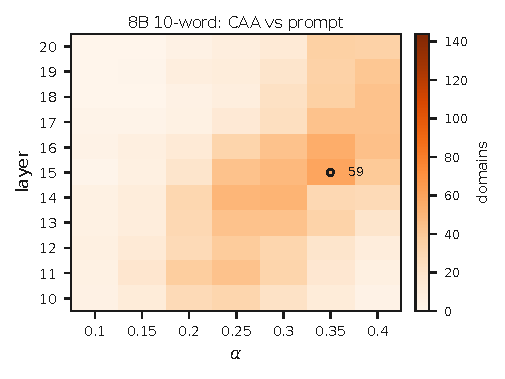
\includegraphics[width=0.62\linewidth]{figures/fig_grid_10w.pdf}
\end{center}
\caption{Llama-3.1-8B-Instruct, 10-word CAA grid.
Domains with $\geq 8/15$ CAA vs.\ prompt item wins at each cell, no per-domain selection.
Circled cell: 59/144.}
\label{fig:grid-10w}
\end{figure}

\section{Per-domain best cells}

Tables~\ref{tab:app-8b-10w}--\ref{tab:app-3b} list every domain's best of 77 cells.
$w$ is item wins out of 15; majority is $\geq 8$.
Prompt+CAA vs.\ prompt fails majority in three 8B four-arm domains, all at 7/15: 3201 Cardiovascular medicine and haematology; 4208 Traditional, complementary and integrative medicine; 5103 Classical physics.
CAA vs.\ prompt fails majority in 31 domains on the 10-word 8B grid and in 41 on the 20-word four-arm grid.

\begingroup
\scriptsize
\setlength{\tabcolsep}{3pt}
\setlength{\LTcapwidth}{\textwidth}

\begin{longtable}{r p{3.35cm} rr r rrr}
\caption{Llama-3.1-8B-Instruct, 10-word CAA grid. Per-domain best cell for CAA vs.\ prompt.}
\label{tab:app-8b-10w} \\
\toprule
ID & Domain & $L$ & $\alpha$ & $w$ & CAA sim & prompt sim & silent sim \\
\midrule
\endfirsthead
\toprule
ID & Domain & $L$ & $\alpha$ & $w$ & CAA sim & prompt sim & silent sim \\
\midrule
\endhead
\midrule
\multicolumn{8}{r}{\emph{continued on next page}} \\
\endfoot
\bottomrule
\endlastfoot
3001 & Agricultural biotechnology & 12 & 0.25 & 12 & 0.558 & 0.482 & 0.314 \\
3002 & Agriculture, land and farm management & 15 & 0.35 & 9 & 0.424 & 0.447 & 0.262 \\
3003 & Animal production & 10 & 0.3 & 11 & 0.458 & 0.410 & 0.281 \\
3004 & Crop and pasture production & 16 & 0.35 & 9 & 0.472 & 0.492 & 0.269 \\
3005 & Fisheries sciences & 16 & 0.35 & 8 & 0.539 & 0.544 & 0.306 \\
3007 & Forestry sciences & 19 & 0.3 & 11 & 0.554 & 0.489 & 0.366 \\
3008 & Horticultural production & 19 & 0.4 & 10 & 0.498 & 0.491 & 0.247 \\
3009 & Veterinary sciences & 10 & 0.25 & 11 & 0.447 & 0.427 & 0.276 \\
3101 & Biochemistry and cell biology & 15 & 0.3 & 12 & 0.675 & 0.621 & 0.417 \\
3102 & Bioinformatics and computational biology & 18 & 0.4 & 11 & 0.591 & 0.563 & 0.355 \\
3104 & Evolutionary biology & 19 & 0.4 & 11 & 0.491 & 0.426 & 0.263 \\
3106 & Industrial biotechnology & 11 & 0.25 & 12 & 0.531 & 0.456 & 0.327 \\
3107 & Microbiology & 13 & 0.25 & 5 & 0.503 & 0.576 & 0.327 \\
3108 & Plant biology & 16 & 0.4 & 7 & 0.558 & 0.611 & 0.379 \\
3109 & Zoology & 17 & 0.35 & 9 & 0.467 & 0.478 & 0.404 \\
3201 & Cardiovascular medicine and haematology & 11 & 0.2 & 8 & 0.442 & 0.498 & 0.292 \\
3202 & Clinical sciences & 13 & 0.3 & 11 & 0.442 & 0.407 & 0.341 \\
3203 & Dentistry & 11 & 0.25 & 9 & 0.551 & 0.529 & 0.302 \\
3204 & Immunology & 17 & 0.35 & 10 & 0.522 & 0.485 & 0.207 \\
3205 & Medical biochemistry and metabolomics & 14 & 0.3 & 10 & 0.500 & 0.493 & 0.329 \\
3206 & Medical biotechnology & 12 & 0.2 & 11 & 0.635 & 0.561 & 0.379 \\
3207 & Medical microbiology & 14 & 0.3 & 13 & 0.597 & 0.529 & 0.349 \\
3208 & Medical physiology & 15 & 0.4 & 9 & 0.524 & 0.512 & 0.440 \\
3209 & Neurosciences & 14 & 0.3 & 11 & 0.586 & 0.498 & 0.348 \\
3210 & Nutrition and dietetics & 15 & 0.35 & 8 & 0.582 & 0.596 & 0.330 \\
3211 & Oncology and carcinogenesis & 16 & 0.3 & 9 & 0.438 & 0.431 & 0.243 \\
3212 & Ophthalmology and optometry & 11 & 0.25 & 10 & 0.640 & 0.566 & 0.380 \\
3213 & Paediatrics & 17 & 0.4 & 7 & 0.451 & 0.484 & 0.337 \\
3214 & Pharmacology and pharmaceutical sciences & 14 & 0.25 & 9 & 0.507 & 0.532 & 0.349 \\
3215 & Reproductive medicine & 20 & 0.4 & 10 & 0.415 & 0.385 & 0.273 \\
3304 & Urban and regional planning & 17 & 0.35 & 8 & 0.565 & 0.586 & 0.355 \\
3401 & Analytical chemistry & 11 & 0.25 & 10 & 0.704 & 0.672 & 0.524 \\
3402 & Inorganic chemistry & 15 & 0.3 & 13 & 0.558 & 0.497 & 0.372 \\
3403 & Macromolecular and materials chemistry & 15 & 0.35 & 9 & 0.510 & 0.556 & 0.433 \\
3404 & Medicinal and biomolecular chemistry & 12 & 0.25 & 12 & 0.504 & 0.424 & 0.297 \\
3405 & Organic chemistry & 15 & 0.3 & 9 & 0.437 & 0.422 & 0.267 \\
3406 & Physical chemistry & 11 & 0.2 & 7 & 0.467 & 0.491 & 0.364 \\
3407 & Theoretical and computational chemistry & 11 & 0.2 & 10 & 0.377 & 0.366 & 0.277 \\
3501 & Accounting, auditing and accountability & 10 & 0.3 & 6 & 0.483 & 0.535 & 0.325 \\
3502 & Banking, finance and investment & 11 & 0.25 & 6 & 0.516 & 0.561 & 0.431 \\
3503 & Business systems in context & 15 & 0.4 & 8 & 0.455 & 0.453 & 0.395 \\
3504 & Commercial services & 19 & 0.4 & 11 & 0.479 & 0.467 & 0.442 \\
3505 & Human resources and industrial relations & 11 & 0.3 & 9 & 0.519 & 0.537 & 0.379 \\
3507 & Strategy, management and organisational behaviour & 17 & 0.35 & 7 & 0.544 & 0.556 & 0.429 \\
3509 & Transportation, logistics and supply chains & 11 & 0.2 & 7 & 0.562 & 0.588 & 0.451 \\
3601 & Art history, theory and criticism & 15 & 0.2 & 8 & 0.455 & 0.488 & 0.413 \\
3602 & Creative and professional writing & 17 & 0.4 & 11 & 0.450 & 0.368 & 0.323 \\
3604 & Performing arts & 11 & 0.25 & 10 & 0.507 & 0.484 & 0.381 \\
3605 & Screen and digital media & 15 & 0.35 & 12 & 0.478 & 0.413 & 0.341 \\
3606 & Visual arts & 18 & 0.3 & 8 & 0.312 & 0.342 & 0.286 \\
3702 & Climate change science & 11 & 0.25 & 10 & 0.484 & 0.443 & 0.288 \\
3704 & Geoinformatics & 15 & 0.35 & 7 & 0.476 & 0.477 & 0.364 \\
3705 & Geology & 15 & 0.25 & 8 & 0.538 & 0.554 & 0.388 \\
3706 & Geophysics & 20 & 0.25 & 11 & 0.432 & 0.446 & 0.353 \\
3708 & Oceanography & 14 & 0.35 & 9 & 0.510 & 0.509 & 0.317 \\
3709 & Physical geography and environmental geoscience & 15 & 0.35 & 8 & 0.549 & 0.577 & 0.347 \\
3801 & Applied economics & 18 & 0.35 & 8 & 0.432 & 0.448 & 0.327 \\
3803 & Economic theory & 14 & 0.3 & 8 & 0.499 & 0.486 & 0.394 \\
3901 & Curriculum and pedagogy & 20 & 0.4 & 5 & 0.516 & 0.577 & 0.405 \\
3902 & Education policy, sociology and philosophy & 18 & 0.4 & 7 & 0.469 & 0.515 & 0.340 \\
3903 & Education systems & 14 & 0.3 & 11 & 0.547 & 0.491 & 0.379 \\
3904 & Specialist studies in education & 15 & 0.35 & 10 & 0.614 & 0.569 & 0.431 \\
4001 & Aerospace engineering & 10 & 0.2 & 9 & 0.342 & 0.362 & 0.264 \\
4002 & Automotive engineering & 19 & 0.3 & 7 & 0.476 & 0.519 & 0.350 \\
4003 & Biomedical engineering & 15 & 0.35 & 10 & 0.449 & 0.417 & 0.310 \\
4004 & Chemical engineering & 11 & 0.3 & 8 & 0.372 & 0.377 & 0.284 \\
4005 & Civil engineering & 12 & 0.4 & 9 & 0.381 & 0.411 & 0.331 \\
4006 & Communications engineering & 16 & 0.4 & 10 & 0.532 & 0.511 & 0.346 \\
4007 & Control engineering, mechatronics and robotics & 19 & 0.4 & 9 & 0.435 & 0.460 & 0.351 \\
4008 & Electrical engineering & 12 & 0.2 & 6 & 0.498 & 0.552 & 0.344 \\
4009 & Electronics, sensors and digital hardware & 12 & 0.25 & 10 & 0.421 & 0.400 & 0.315 \\
4010 & Engineering practice and education & 18 & 0.4 & 9 & 0.401 & 0.411 & 0.360 \\
4011 & Environmental engineering & 15 & 0.25 & 11 & 0.462 & 0.452 & 0.318 \\
4012 & Fluid mechanics and thermal engineering & 10 & 0.2 & 9 & 0.533 & 0.544 & 0.372 \\
4013 & Geomatic engineering & 12 & 0.2 & 7 & 0.484 & 0.514 & 0.420 \\
4014 & Manufacturing engineering & 12 & 0.35 & 9 & 0.447 & 0.439 & 0.306 \\
4015 & Maritime engineering & 19 & 0.4 & 7 & 0.574 & 0.614 & 0.411 \\
4016 & Materials engineering & 15 & 0.35 & 9 & 0.511 & 0.546 & 0.354 \\
4018 & Nanotechnology & 16 & 0.4 & 11 & 0.512 & 0.431 & 0.307 \\
4019 & Resources engineering and extractive metallurgy & 17 & 0.35 & 6 & 0.451 & 0.459 & 0.317 \\
4101 & Climate change impacts and adaptation & 12 & 0.25 & 7 & 0.485 & 0.513 & 0.368 \\
4102 & Ecological applications & 11 & 0.25 & 10 & 0.531 & 0.490 & 0.319 \\
4103 & Environmental biotechnology & 16 & 0.35 & 8 & 0.373 & 0.400 & 0.244 \\
4104 & Environmental management & 17 & 0.4 & 10 & 0.535 & 0.511 & 0.392 \\
4105 & Pollution and contamination & 11 & 0.3 & 11 & 0.490 & 0.415 & 0.281 \\
4106 & Soil sciences & 15 & 0.25 & 8 & 0.649 & 0.652 & 0.335 \\
4201 & Allied health and rehabilitation science & 13 & 0.3 & 8 & 0.384 & 0.402 & 0.318 \\
4203 & Health services and systems & 17 & 0.4 & 8 & 0.543 & 0.530 & 0.355 \\
4206 & Public health & 13 & 0.25 & 10 & 0.561 & 0.554 & 0.453 \\
4207 & Sports science and exercise & 18 & 0.4 & 10 & 0.452 & 0.419 & 0.307 \\
4208 & Traditional, complementary and integrative medicine & 18 & 0.4 & 9 & 0.387 & 0.464 & 0.361 \\
4302 & Heritage, archive and museum studies & 14 & 0.3 & 7 & 0.441 & 0.450 & 0.337 \\
4303 & Historical studies & 15 & 0.25 & 8 & 0.561 & 0.580 & 0.518 \\
4404 & Development studies & 19 & 0.4 & 7 & 0.484 & 0.531 & 0.376 \\
4405 & Gender studies & 16 & 0.4 & 11 & 0.398 & 0.385 & 0.288 \\
4406 & Human geography & 13 & 0.35 & 10 & 0.487 & 0.488 & 0.404 \\
4407 & Policy and administration & 14 & 0.3 & 11 & 0.479 & 0.450 & 0.396 \\
4408 & Political science & 15 & 0.4 & 9 & 0.568 & 0.554 & 0.382 \\
4601 & Applied computing & 17 & 0.4 & 9 & 0.403 & 0.407 & 0.368 \\
4602 & Artificial intelligence & 13 & 0.4 & 12 & 0.468 & 0.427 & 0.393 \\
4603 & Computer vision and multimedia computation & 15 & 0.35 & 9 & 0.478 & 0.473 & 0.365 \\
4604 & Cybersecurity and privacy & 13 & 0.25 & 13 & 0.634 & 0.586 & 0.458 \\
4605 & Data management and data science & 15 & 0.35 & 8 & 0.456 & 0.441 & 0.326 \\
4606 & Distributed computing and systems software & 16 & 0.3 & 10 & 0.411 & 0.404 & 0.319 \\
4607 & Graphics, augmented reality and games & 13 & 0.35 & 11 & 0.449 & 0.448 & 0.331 \\
4608 & Human-centred computing & 14 & 0.3 & 12 & 0.505 & 0.467 & 0.368 \\
4610 & Library and information studies & 11 & 0.4 & 10 & 0.419 & 0.398 & 0.329 \\
4611 & Machine learning & 16 & 0.35 & 12 & 0.461 & 0.401 & 0.331 \\
4612 & Software engineering & 14 & 0.25 & 11 & 0.555 & 0.516 & 0.387 \\
4613 & Theory of computation & 16 & 0.35 & 8 & 0.406 & 0.414 & 0.362 \\
4701 & Communication and media studies & 14 & 0.25 & 7 & 0.443 & 0.508 & 0.295 \\
4702 & Cultural studies & 16 & 0.35 & 11 & 0.638 & 0.594 & 0.458 \\
4703 & Language studies & 13 & 0.2 & 12 & 0.497 & 0.461 & 0.397 \\
4705 & Literary studies & 15 & 0.3 & 13 & 0.498 & 0.450 & 0.465 \\
4801 & Commercial law & 10 & 0.25 & 8 & 0.522 & 0.524 & 0.453 \\
4802 & Environmental and resources law & 10 & 0.25 & 9 & 0.451 & 0.487 & 0.367 \\
4803 & International and comparative law & 10 & 0.3 & 8 & 0.496 & 0.496 & 0.332 \\
4804 & Law in context & 19 & 0.4 & 7 & 0.507 & 0.600 & 0.438 \\
4805 & Legal systems & 11 & 0.2 & 7 & 0.452 & 0.549 & 0.391 \\
4806 & Private law and civil obligations & 16 & 0.35 & 5 & 0.510 & 0.575 & 0.447 \\
4807 & Public law & 17 & 0.3 & 11 & 0.493 & 0.441 & 0.434 \\
4901 & Applied mathematics & 13 & 0.3 & 10 & 0.404 & 0.381 & 0.338 \\
4902 & Mathematical physics & 15 & 0.35 & 9 & 0.423 & 0.415 & 0.263 \\
4903 & Numerical and computational mathematics & 16 & 0.25 & 8 & 0.355 & 0.395 & 0.274 \\
4904 & Pure mathematics & 14 & 0.25 & 8 & 0.432 & 0.453 & 0.374 \\
4905 & Statistics & 12 & 0.25 & 4 & 0.449 & 0.488 & 0.327 \\
5001 & Applied ethics & 16 & 0.4 & 8 & 0.590 & 0.580 & 0.509 \\
5002 & History and philosophy of specific fields & 19 & 0.4 & 10 & 0.547 & 0.530 & 0.472 \\
5003 & Philosophy & 16 & 0.25 & 8 & 0.524 & 0.513 & 0.458 \\
5101 & Astronomical sciences & 13 & 0.25 & 7 & 0.694 & 0.734 & 0.462 \\
5102 & Atomic, molecular and optical physics & 19 & 0.4 & 9 & 0.414 & 0.450 & 0.339 \\
5103 & Classical physics & 16 & 0.1 & 6 & 0.525 & 0.586 & 0.510 \\
5104 & Condensed matter physics & 14 & 0.25 & 5 & 0.450 & 0.490 & 0.310 \\
5105 & Medical and biological physics & 16 & 0.4 & 10 & 0.384 & 0.379 & 0.319 \\
5106 & Nuclear and plasma physics & 17 & 0.3 & 7 & 0.499 & 0.508 & 0.343 \\
5107 & Particle and high energy physics & 17 & 0.35 & 8 & 0.420 & 0.440 & 0.278 \\
5108 & Quantum physics & 15 & 0.2 & 8 & 0.400 & 0.466 & 0.362 \\
5109 & Space sciences & 14 & 0.25 & 10 & 0.424 & 0.420 & 0.299 \\
5110 & Synchrotrons and accelerators & 17 & 0.35 & 8 & 0.465 & 0.481 & 0.318 \\
5201 & Applied and developmental psychology & 17 & 0.35 & 12 & 0.443 & 0.422 & 0.408 \\
5202 & Biological psychology & 15 & 0.25 & 6 & 0.460 & 0.542 & 0.376 \\
5203 & Clinical and health psychology & 16 & 0.4 & 7 & 0.442 & 0.474 & 0.312 \\
5204 & Cognitive and computational psychology & 14 & 0.4 & 9 & 0.438 & 0.427 & 0.337 \\
5205 & Social and personality psychology & 14 & 0.3 & 6 & 0.466 & 0.527 & 0.352 \\
\end{longtable}
{\small $w$: CAA item wins vs.\ the domain prompt / 15. Majority ($\geq 8$): 113/144.}


\vspace{1.2em}
\begin{longtable}{r p{2.15cm} rrr rrr rrr}
\caption{Llama-3.1-8B-Instruct, 20-word four-arm grid. Per-domain best cell for each comparison (layer $L$, strength $\alpha$, item wins $w$).}
\label{tab:app-8b-20w} \\
\toprule
ID & Domain & \multicolumn{3}{c}{CAA vs silent} & \multicolumn{3}{c}{CAA vs prompt} & \multicolumn{3}{c}{p+CAA vs prompt} \\
\cmidrule(lr){3-5}\cmidrule(lr){6-8}\cmidrule(lr){9-11}
 & & $L$ & $\alpha$ & $w$ & $L$ & $\alpha$ & $w$ & $L$ & $\alpha$ & $w$ \\
\midrule
\endfirsthead
\toprule
ID & Domain & \multicolumn{3}{c}{CAA vs silent} & \multicolumn{3}{c}{CAA vs prompt} & \multicolumn{3}{c}{p+CAA vs prompt} \\
\cmidrule(lr){3-5}\cmidrule(lr){6-8}\cmidrule(lr){9-11}
 & & $L$ & $\alpha$ & $w$ & $L$ & $\alpha$ & $w$ & $L$ & $\alpha$ & $w$ \\
\midrule
\endhead
\midrule
\multicolumn{11}{r}{\emph{continued on next page}} \\
\endfoot
\bottomrule
\endlastfoot
3001 & Agricultural biotechnology & 16 & 0.35 & 15 & 13 & 0.3 & 12 & 13 & 0.2 & 12 \\
3002 & Agriculture, land and farm management & 15 & 0.35 & 15 & 11 & 0.3 & 11 & 14 & 0.2 & 12 \\
3003 & Animal production & 15 & 0.35 & 15 & 16 & 0.4 & 8 & 18 & 0.1 & 13 \\
3004 & Crop and pasture production & 17 & 0.4 & 15 & 12 & 0.25 & 8 & 20 & 0.25 & 10 \\
3005 & Fisheries sciences & 19 & 0.4 & 15 & 15 & 0.3 & 3 & 19 & 0.2 & 8 \\
3007 & Forestry sciences & 10 & 0.25 & 14 & 16 & 0.2 & 9 & 13 & 0.15 & 9 \\
3008 & Horticultural production & 11 & 0.2 & 15 & 10 & 0.2 & 12 & 14 & 0.2 & 11 \\
3009 & Veterinary sciences & 14 & 0.35 & 15 & 12 & 0.25 & 9 & 13 & 0.15 & 13 \\
3101 & Biochemistry and cell biology & 17 & 0.35 & 15 & 15 & 0.3 & 10 & 19 & 0.2 & 13 \\
3102 & Bioinformatics and computational biology & 11 & 0.25 & 15 & 15 & 0.3 & 10 & 17 & 0.2 & 11 \\
3104 & Evolutionary biology & 10 & 0.25 & 15 & 13 & 0.3 & 7 & 17 & 0.35 & 11 \\
3106 & Industrial biotechnology & 10 & 0.25 & 15 & 10 & 0.25 & 9 & 11 & 0.15 & 10 \\
3107 & Microbiology & 15 & 0.25 & 15 & 19 & 0.35 & 4 & 18 & 0.2 & 10 \\
3108 & Plant biology & 17 & 0.35 & 15 & 11 & 0.3 & 7 & 18 & 0.25 & 10 \\
3109 & Zoology & 13 & 0.15 & 14 & 17 & 0.4 & 11 & 12 & 0.15 & 12 \\
3201 & Cardiovascular medicine and haematology & 11 & 0.2 & 14 & 10 & 0.2 & 7 & 20 & 0.1 & 7 \\
3202 & Clinical sciences & 10 & 0.2 & 15 & 15 & 0.3 & 13 & 16 & 0.2 & 13 \\
3203 & Dentistry & 10 & 0.3 & 15 & 10 & 0.3 & 11 & 10 & 0.15 & 13 \\
3204 & Immunology & 19 & 0.4 & 15 & 17 & 0.35 & 10 & 12 & 0.1 & 13 \\
3205 & Medical biochemistry and metabolomics & 14 & 0.25 & 15 & 16 & 0.3 & 8 & 14 & 0.2 & 11 \\
3206 & Medical biotechnology & 11 & 0.25 & 15 & 16 & 0.4 & 12 & 13 & 0.2 & 12 \\
3207 & Medical microbiology & 15 & 0.35 & 15 & 12 & 0.2 & 10 & 17 & 0.3 & 13 \\
3208 & Medical physiology & 15 & 0.3 & 13 & 20 & 0.35 & 10 & 12 & 0.2 & 11 \\
3209 & Neurosciences & 13 & 0.25 & 15 & 13 & 0.25 & 11 & 12 & 0.15 & 11 \\
3210 & Nutrition and dietetics & 11 & 0.25 & 15 & 16 & 0.3 & 8 & 15 & 0.15 & 12 \\
3211 & Oncology and carcinogenesis & 20 & 0.35 & 15 & 20 & 0.35 & 9 & 18 & 0.2 & 10 \\
3212 & Ophthalmology and optometry & 15 & 0.3 & 15 & 11 & 0.25 & 10 & 11 & 0.25 & 11 \\
3213 & Paediatrics & 15 & 0.25 & 14 & 19 & 0.4 & 7 & 17 & 0.25 & 10 \\
3214 & Pharmacology and pharmaceutical sciences & 10 & 0.2 & 15 & 10 & 0.2 & 7 & 16 & 0.25 & 10 \\
3215 & Reproductive medicine & 16 & 0.3 & 15 & 11 & 0.3 & 9 & 13 & 0.15 & 11 \\
3304 & Urban and regional planning & 14 & 0.35 & 15 & 15 & 0.4 & 8 & 15 & 0.15 & 11 \\
3401 & Analytical chemistry & 10 & 0.25 & 14 & 15 & 0.3 & 10 & 14 & 0.15 & 11 \\
3402 & Inorganic chemistry & 12 & 0.25 & 15 & 13 & 0.2 & 12 & 16 & 0.1 & 11 \\
3403 & Macromolecular and materials chemistry & 14 & 0.25 & 15 & 17 & 0.3 & 8 & 11 & 0.1 & 11 \\
3404 & Medicinal and biomolecular chemistry & 12 & 0.25 & 15 & 12 & 0.25 & 10 & 18 & 0.3 & 13 \\
3405 & Organic chemistry & 11 & 0.2 & 15 & 11 & 0.2 & 8 & 13 & 0.1 & 10 \\
3406 & Physical chemistry & 11 & 0.25 & 14 & 11 & 0.2 & 8 & 11 & 0.15 & 12 \\
3407 & Theoretical and computational chemistry & 11 & 0.25 & 14 & 16 & 0.35 & 10 & 12 & 0.1 & 12 \\
3501 & Accounting, auditing and accountability & 10 & 0.25 & 15 & 10 & 0.25 & 6 & 10 & 0.15 & 10 \\
3502 & Banking, finance and investment & 12 & 0.25 & 13 & 12 & 0.2 & 7 & 14 & 0.15 & 13 \\
3503 & Business systems in context & 13 & 0.25 & 13 & 13 & 0.25 & 8 & 18 & 0.1 & 9 \\
3504 & Commercial services & 15 & 0.25 & 15 & 15 & 0.25 & 12 & 18 & 0.3 & 13 \\
3505 & Human resources and industrial relations & 17 & 0.4 & 15 & 11 & 0.25 & 9 & 10 & 0.2 & 11 \\
3507 & Strategy, management and organisational behaviour & 19 & 0.35 & 14 & 18 & 0.4 & 6 & 20 & 0.1 & 10 \\
3509 & Transportation, logistics and supply chains & 10 & 0.15 & 14 & 11 & 0.2 & 7 & 15 & 0.2 & 10 \\
3601 & Art history, theory and criticism & 11 & 0.25 & 13 & 12 & 0.3 & 9 & 20 & 0.1 & 9 \\
3602 & Creative and professional writing & 13 & 0.3 & 13 & 10 & 0.3 & 11 & 15 & 0.35 & 11 \\
3604 & Performing arts & 14 & 0.2 & 14 & 14 & 0.25 & 11 & 15 & 0.2 & 12 \\
3605 & Screen and digital media & 10 & 0.3 & 15 & 15 & 0.35 & 13 & 15 & 0.2 & 10 \\
3606 & Visual arts & 15 & 0.3 & 14 & 16 & 0.4 & 6 & 18 & 0.4 & 12 \\
3702 & Climate change science & 10 & 0.3 & 15 & 12 & 0.25 & 7 & 11 & 0.1 & 10 \\
3704 & Geoinformatics & 13 & 0.3 & 14 & 13 & 0.3 & 8 & 10 & 0.1 & 11 \\
3705 & Geology & 16 & 0.25 & 14 & 15 & 0.25 & 7 & 16 & 0.1 & 12 \\
3706 & Geophysics & 10 & 0.2 & 12 & 10 & 0.2 & 7 & 10 & 0.25 & 11 \\
3708 & Oceanography & 12 & 0.25 & 15 & 12 & 0.25 & 9 & 16 & 0.3 & 13 \\
3709 & Physical geography and environmental geoscience & 12 & 0.25 & 15 & 10 & 0.25 & 11 & 18 & 0.25 & 14 \\
3801 & Applied economics & 16 & 0.3 & 13 & 12 & 0.25 & 9 & 12 & 0.2 & 11 \\
3803 & Economic theory & 11 & 0.25 & 13 & 10 & 0.25 & 7 & 16 & 0.15 & 11 \\
3901 & Curriculum and pedagogy & 11 & 0.15 & 13 & 15 & 0.25 & 5 & 12 & 0.1 & 8 \\
3902 & Education policy, sociology and philosophy & 11 & 0.25 & 13 & 11 & 0.25 & 7 & 13 & 0.1 & 9 \\
3903 & Education systems & 19 & 0.4 & 14 & 19 & 0.4 & 11 & 11 & 0.25 & 12 \\
3904 & Specialist studies in education & 16 & 0.2 & 15 & 16 & 0.2 & 12 & 10 & 0.25 & 12 \\
4001 & Aerospace engineering & 13 & 0.35 & 15 & 10 & 0.3 & 12 & 13 & 0.15 & 14 \\
4002 & Automotive engineering & 15 & 0.3 & 15 & 15 & 0.3 & 7 & 20 & 0.1 & 10 \\
4003 & Biomedical engineering & 13 & 0.35 & 15 & 15 & 0.35 & 9 & 16 & 0.3 & 11 \\
4004 & Chemical engineering & 13 & 0.3 & 14 & 10 & 0.3 & 10 & 13 & 0.2 & 12 \\
4005 & Civil engineering & 16 & 0.4 & 14 & 13 & 0.35 & 11 & 18 & 0.35 & 12 \\
4006 & Communications engineering & 11 & 0.25 & 15 & 14 & 0.25 & 12 & 12 & 0.2 & 13 \\
4007 & Control engineering, mechatronics and robotics & 16 & 0.3 & 15 & 13 & 0.25 & 8 & 10 & 0.15 & 12 \\
4008 & Electrical engineering & 10 & 0.25 & 15 & 10 & 0.25 & 7 & 13 & 0.1 & 11 \\
4009 & Electronics, sensors and digital hardware & 14 & 0.25 & 15 & 13 & 0.3 & 11 & 10 & 0.3 & 12 \\
4010 & Engineering practice and education & 16 & 0.4 & 12 & 14 & 0.35 & 8 & 20 & 0.3 & 9 \\
4011 & Environmental engineering & 15 & 0.3 & 14 & 15 & 0.3 & 10 & 14 & 0.1 & 13 \\
4012 & Fluid mechanics and thermal engineering & 12 & 0.25 & 15 & 11 & 0.3 & 7 & 17 & 0.1 & 11 \\
4013 & Geomatic engineering & 16 & 0.25 & 12 & 15 & 0.3 & 9 & 10 & 0.15 & 11 \\
4014 & Manufacturing engineering & 10 & 0.3 & 15 & 10 & 0.3 & 10 & 10 & 0.25 & 12 \\
4015 & Maritime engineering & 16 & 0.25 & 14 & 18 & 0.4 & 10 & 17 & 0.2 & 11 \\
4016 & Materials engineering & 16 & 0.25 & 15 & 12 & 0.3 & 9 & 18 & 0.1 & 11 \\
4018 & Nanotechnology & 13 & 0.3 & 15 & 13 & 0.3 & 11 & 13 & 0.2 & 11 \\
4019 & Resources engineering and extractive metallurgy & 20 & 0.4 & 14 & 16 & 0.25 & 5 & 19 & 0.1 & 8 \\
4101 & Climate change impacts and adaptation & 16 & 0.4 & 13 & 13 & 0.3 & 5 & 12 & 0.2 & 10 \\
4102 & Ecological applications & 17 & 0.4 & 15 & 17 & 0.35 & 9 & 19 & 0.2 & 11 \\
4103 & Environmental biotechnology & 11 & 0.3 & 15 & 14 & 0.35 & 10 & 11 & 0.1 & 14 \\
4104 & Environmental management & 16 & 0.4 & 15 & 16 & 0.4 & 12 & 13 & 0.2 & 13 \\
4105 & Pollution and contamination & 14 & 0.4 & 15 & 14 & 0.4 & 10 & 16 & 0.4 & 12 \\
4106 & Soil sciences & 12 & 0.25 & 15 & 13 & 0.25 & 7 & 20 & 0.15 & 9 \\
4201 & Allied health and rehabilitation science & 13 & 0.25 & 14 & 12 & 0.3 & 9 & 10 & 0.2 & 9 \\
4203 & Health services and systems & 18 & 0.35 & 14 & 15 & 0.25 & 7 & 14 & 0.2 & 9 \\
4206 & Public health & 12 & 0.2 & 15 & 12 & 0.15 & 10 & 12 & 0.1 & 13 \\
4207 & Sports science and exercise & 14 & 0.25 & 14 & 14 & 0.25 & 6 & 16 & 0.2 & 8 \\
4208 & Traditional, complementary and integrative medicine & 13 & 0.3 & 13 & 17 & 0.35 & 6 & 10 & 0.15 & 7 \\
4302 & Heritage, archive and museum studies & 11 & 0.3 & 14 & 11 & 0.3 & 6 & 14 & 0.15 & 8 \\
4303 & Historical studies & 15 & 0.3 & 13 & 15 & 0.3 & 11 & 10 & 0.2 & 10 \\
4404 & Development studies & 16 & 0.4 & 14 & 14 & 0.4 & 10 & 17 & 0.3 & 12 \\
4405 & Gender studies & 10 & 0.2 & 14 & 10 & 0.3 & 11 & 18 & 0.15 & 14 \\
4406 & Human geography & 15 & 0.25 & 12 & 13 & 0.25 & 8 & 13 & 0.15 & 10 \\
4407 & Policy and administration & 13 & 0.4 & 14 & 10 & 0.3 & 11 & 10 & 0.2 & 10 \\
4408 & Political science & 17 & 0.4 & 15 & 17 & 0.35 & 9 & 10 & 0.15 & 11 \\
4601 & Applied computing & 18 & 0.1 & 12 & 15 & 0.15 & 9 & 19 & 0.25 & 8 \\
4602 & Artificial intelligence & 12 & 0.25 & 13 & 16 & 0.25 & 10 & 13 & 0.25 & 10 \\
4603 & Computer vision and multimedia computation & 13 & 0.3 & 15 & 15 & 0.3 & 5 & 17 & 0.1 & 10 \\
4604 & Cybersecurity and privacy & 13 & 0.25 & 15 & 12 & 0.3 & 11 & 15 & 0.1 & 13 \\
4605 & Data management and data science & 15 & 0.35 & 15 & 16 & 0.35 & 9 & 17 & 0.3 & 11 \\
4606 & Distributed computing and systems software & 13 & 0.3 & 14 & 13 & 0.3 & 11 & 12 & 0.1 & 10 \\
4607 & Graphics, augmented reality and games & 12 & 0.25 & 15 & 15 & 0.3 & 13 & 14 & 0.25 & 13 \\
4608 & Human-centred computing & 16 & 0.3 & 15 & 16 & 0.3 & 9 & 14 & 0.2 & 12 \\
4610 & Library and information studies & 10 & 0.3 & 15 & 10 & 0.3 & 9 & 18 & 0.1 & 12 \\
4611 & Machine learning & 14 & 0.25 & 15 & 10 & 0.2 & 11 & 16 & 0.3 & 11 \\
4612 & Software engineering & 10 & 0.3 & 15 & 10 & 0.3 & 10 & 20 & 0.2 & 11 \\
4613 & Theory of computation & 15 & 0.15 & 13 & 12 & 0.2 & 9 & 19 & 0.2 & 8 \\
4701 & Communication and media studies & 13 & 0.4 & 15 & 14 & 0.3 & 6 & 18 & 0.3 & 9 \\
4702 & Cultural studies & 16 & 0.3 & 15 & 16 & 0.35 & 10 & 17 & 0.3 & 12 \\
4703 & Language studies & 12 & 0.3 & 13 & 12 & 0.3 & 10 & 10 & 0.2 & 12 \\
4705 & Literary studies & 10 & 0.1 & 11 & 13 & 0.15 & 10 & 15 & 0.15 & 11 \\
4801 & Commercial law & 18 & 0.4 & 13 & 16 & 0.35 & 9 & 11 & 0.1 & 9 \\
4802 & Environmental and resources law & 19 & 0.4 & 15 & 14 & 0.25 & 6 & 20 & 0.2 & 10 \\
4803 & International and comparative law & 15 & 0.3 & 14 & 15 & 0.3 & 8 & 16 & 0.2 & 11 \\
4804 & Law in context & 17 & 0.35 & 14 & 17 & 0.4 & 8 & 17 & 0.25 & 11 \\
4805 & Legal systems & 18 & 0.4 & 13 & 15 & 0.25 & 9 & 17 & 0.15 & 14 \\
4806 & Private law and civil obligations & 19 & 0.3 & 14 & 15 & 0.25 & 7 & 16 & 0.25 & 8 \\
4807 & Public law & 17 & 0.4 & 12 & 13 & 0.25 & 9 & 17 & 0.15 & 11 \\
4901 & Applied mathematics & 15 & 0.2 & 12 & 15 & 0.2 & 10 & 20 & 0.15 & 12 \\
4902 & Mathematical physics & 11 & 0.2 & 15 & 15 & 0.3 & 9 & 17 & 0.3 & 12 \\
4903 & Numerical and computational mathematics & 17 & 0.3 & 15 & 16 & 0.3 & 7 & 17 & 0.2 & 9 \\
4904 & Pure mathematics & 15 & 0.2 & 13 & 12 & 0.2 & 8 & 19 & 0.15 & 8 \\
4905 & Statistics & 12 & 0.25 & 13 & 11 & 0.25 & 5 & 10 & 0.2 & 9 \\
5001 & Applied ethics & 16 & 0.4 & 15 & 15 & 0.35 & 7 & 14 & 0.15 & 11 \\
5002 & History and philosophy of specific fields & 11 & 0.25 & 12 & 19 & 0.4 & 8 & 19 & 0.15 & 10 \\
5003 & Philosophy & 16 & 0.25 & 13 & 10 & 0.25 & 9 & 14 & 0.15 & 9 \\
5101 & Astronomical sciences & 18 & 0.25 & 15 & 14 & 0.25 & 8 & 19 & 0.15 & 10 \\
5102 & Atomic, molecular and optical physics & 13 & 0.3 & 14 & 12 & 0.3 & 10 & 13 & 0.1 & 12 \\
5103 & Classical physics & 15 & 0.2 & 10 & 18 & 0.15 & 6 & 16 & 0.15 & 7 \\
5104 & Condensed matter physics & 13 & 0.2 & 13 & 15 & 0.3 & 5 & 11 & 0.1 & 8 \\
5105 & Medical and biological physics & 13 & 0.3 & 13 & 10 & 0.3 & 10 & 19 & 0.35 & 9 \\
5106 & Nuclear and plasma physics & 11 & 0.2 & 15 & 11 & 0.2 & 10 & 16 & 0.2 & 13 \\
5107 & Particle and high energy physics & 19 & 0.35 & 14 & 18 & 0.35 & 8 & 14 & 0.1 & 12 \\
5108 & Quantum physics & 14 & 0.15 & 14 & 18 & 0.35 & 7 & 17 & 0.15 & 9 \\
5109 & Space sciences & 19 & 0.4 & 14 & 12 & 0.2 & 7 & 17 & 0.15 & 10 \\
5110 & Synchrotrons and accelerators & 11 & 0.25 & 15 & 15 & 0.4 & 5 & 13 & 0.15 & 11 \\
5201 & Applied and developmental psychology & 17 & 0.15 & 12 & 16 & 0.3 & 10 & 15 & 0.25 & 10 \\
5202 & Biological psychology & 20 & 0.3 & 13 & 16 & 0.2 & 8 & 15 & 0.1 & 10 \\
5203 & Clinical and health psychology & 13 & 0.4 & 14 & 14 & 0.35 & 9 & 11 & 0.2 & 12 \\
5204 & Cognitive and computational psychology & 15 & 0.4 & 15 & 10 & 0.25 & 10 & 10 & 0.2 & 13 \\
5205 & Social and personality psychology & 15 & 0.35 & 15 & 15 & 0.35 & 7 & 14 & 0.15 & 11 \\

\end{longtable}
{\small $w$: item wins / 15 at that domain's best cell. Majority ($\geq 8$): CAA vs silent 144/144; CAA vs prompt 103/144; prompt+CAA vs prompt 141/144.}


\vspace{1.2em}
\begin{longtable}{r p{2.15cm} rrr rrr rrr}
\caption{Llama-3.2-3B-Instruct, 10-word four-arm grid. Per-domain best cell for each comparison (layer $L$, strength $\alpha$, item wins $w$).}
\label{tab:app-3b} \\
\toprule
ID & Domain & \multicolumn{3}{c}{CAA vs silent} & \multicolumn{3}{c}{CAA vs prompt} & \multicolumn{3}{c}{p+CAA vs prompt} \\
\cmidrule(lr){3-5}\cmidrule(lr){6-8}\cmidrule(lr){9-11}
 & & $L$ & $\alpha$ & $w$ & $L$ & $\alpha$ & $w$ & $L$ & $\alpha$ & $w$ \\
\midrule
\endfirsthead
\toprule
ID & Domain & \multicolumn{3}{c}{CAA vs silent} & \multicolumn{3}{c}{CAA vs prompt} & \multicolumn{3}{c}{p+CAA vs prompt} \\
\cmidrule(lr){3-5}\cmidrule(lr){6-8}\cmidrule(lr){9-11}
 & & $L$ & $\alpha$ & $w$ & $L$ & $\alpha$ & $w$ & $L$ & $\alpha$ & $w$ \\
\midrule
\endhead
\midrule
\multicolumn{11}{r}{\emph{continued on next page}} \\
\endfoot
\bottomrule
\endlastfoot
3001 & Agricultural biotechnology & 18 & 0.4 & 14 & 18 & 0.4 & 12 & 15 & 0.2 & 12 \\
3002 & Agriculture, land and farm management & 12 & 0.35 & 14 & 10 & 0.3 & 10 & 12 & 0.3 & 11 \\
3003 & Animal production & 10 & 0.25 & 15 & 10 & 0.25 & 11 & 10 & 0.2 & 12 \\
3004 & Crop and pasture production & 10 & 0.25 & 14 & 10 & 0.25 & 11 & 15 & 0.25 & 11 \\
3005 & Fisheries sciences & 14 & 0.2 & 14 & 13 & 0.2 & 10 & 11 & 0.25 & 11 \\
3007 & Forestry sciences & 18 & 0.35 & 14 & 17 & 0.4 & 10 & 20 & 0.3 & 11 \\
3008 & Horticultural production & 14 & 0.4 & 14 & 13 & 0.25 & 8 & 13 & 0.15 & 11 \\
3009 & Veterinary sciences & 13 & 0.25 & 14 & 12 & 0.25 & 12 & 14 & 0.25 & 12 \\
3101 & Biochemistry and cell biology & 13 & 0.2 & 14 & 17 & 0.35 & 10 & 20 & 0.2 & 11 \\
3102 & Bioinformatics and computational biology & 12 & 0.3 & 14 & 14 & 0.3 & 9 & 15 & 0.3 & 11 \\
3104 & Evolutionary biology & 12 & 0.3 & 15 & 15 & 0.4 & 9 & 12 & 0.25 & 8 \\
3106 & Industrial biotechnology & 13 & 0.25 & 15 & 13 & 0.25 & 10 & 18 & 0.25 & 12 \\
3107 & Microbiology & 13 & 0.3 & 15 & 19 & 0.4 & 6 & 14 & 0.15 & 10 \\
3108 & Plant biology & 12 & 0.25 & 15 & 13 & 0.3 & 9 & 12 & 0.1 & 10 \\
3109 & Zoology & 12 & 0.3 & 12 & 11 & 0.25 & 10 & 20 & 0.4 & 10 \\
3201 & Cardiovascular medicine and haematology & 13 & 0.2 & 15 & 11 & 0.2 & 11 & 12 & 0.15 & 7 \\
3202 & Clinical sciences & 18 & 0.25 & 13 & 18 & 0.3 & 10 & 19 & 0.2 & 11 \\
3203 & Dentistry & 11 & 0.2 & 15 & 10 & 0.2 & 10 & 12 & 0.15 & 13 \\
3204 & Immunology & 11 & 0.2 & 15 & 16 & 0.4 & 12 & 13 & 0.15 & 11 \\
3205 & Medical biochemistry and metabolomics & 13 & 0.25 & 14 & 13 & 0.25 & 10 & 19 & 0.35 & 13 \\
3206 & Medical biotechnology & 12 & 0.2 & 15 & 18 & 0.35 & 12 & 13 & 0.15 & 13 \\
3207 & Medical microbiology & 12 & 0.3 & 14 & 14 & 0.25 & 7 & 19 & 0.35 & 10 \\
3208 & Medical physiology & 12 & 0.15 & 13 & 16 & 0.35 & 9 & 12 & 0.1 & 10 \\
3209 & Neurosciences & 12 & 0.2 & 14 & 14 & 0.2 & 11 & 13 & 0.15 & 11 \\
3210 & Nutrition and dietetics & 13 & 0.25 & 14 & 13 & 0.25 & 7 & 18 & 0.2 & 9 \\
3211 & Oncology and carcinogenesis & 14 & 0.25 & 13 & 14 & 0.25 & 9 & 12 & 0.2 & 9 \\
3212 & Ophthalmology and optometry & 16 & 0.35 & 15 & 14 & 0.25 & 8 & 12 & 0.15 & 9 \\
3213 & Paediatrics & 11 & 0.2 & 12 & 11 & 0.2 & 6 & 20 & 0.2 & 7 \\
3214 & Pharmacology and pharmaceutical sciences & 11 & 0.2 & 14 & 13 & 0.25 & 8 & 16 & 0.35 & 11 \\
3215 & Reproductive medicine & 10 & 0.25 & 14 & 10 & 0.25 & 10 & 18 & 0.3 & 11 \\
3304 & Urban and regional planning & 10 & 0.2 & 15 & 12 & 0.3 & 11 & 15 & 0.35 & 12 \\
3401 & Analytical chemistry & 17 & 0.25 & 15 & 11 & 0.25 & 8 & 20 & 0.35 & 9 \\
3402 & Inorganic chemistry & 11 & 0.25 & 13 & 11 & 0.2 & 11 & 13 & 0.1 & 11 \\
3403 & Macromolecular and materials chemistry & 17 & 0.3 & 12 & 17 & 0.3 & 9 & 14 & 0.1 & 10 \\
3404 & Medicinal and biomolecular chemistry & 13 & 0.25 & 15 & 12 & 0.25 & 12 & 16 & 0.25 & 13 \\
3405 & Organic chemistry & 19 & 0.4 & 13 & 19 & 0.4 & 9 & 17 & 0.1 & 10 \\
3406 & Physical chemistry & 11 & 0.15 & 14 & 14 & 0.2 & 8 & 17 & 0.35 & 11 \\
3407 & Theoretical and computational chemistry & 12 & 0.2 & 13 & 15 & 0.35 & 9 & 16 & 0.1 & 9 \\
3501 & Accounting, auditing and accountability & 10 & 0.3 & 14 & 10 & 0.25 & 9 & 10 & 0.15 & 12 \\
3502 & Banking, finance and investment & 16 & 0.35 & 13 & 12 & 0.25 & 6 & 17 & 0.3 & 10 \\
3503 & Business systems in context & 16 & 0.25 & 13 & 13 & 0.25 & 10 & 17 & 0.2 & 10 \\
3504 & Commercial services & 14 & 0.2 & 10 & 13 & 0.3 & 10 & 18 & 0.4 & 10 \\
3505 & Human resources and industrial relations & 10 & 0.2 & 12 & 19 & 0.3 & 11 & 12 & 0.15 & 13 \\
3507 & Strategy, management and organisational behaviour & 17 & 0.4 & 13 & 17 & 0.4 & 8 & 17 & 0.1 & 10 \\
3509 & Transportation, logistics and supply chains & 10 & 0.3 & 13 & 14 & 0.3 & 10 & 14 & 0.25 & 13 \\
3601 & Art history, theory and criticism & 13 & 0.2 & 12 & 14 & 0.3 & 9 & 14 & 0.2 & 11 \\
3602 & Creative and professional writing & 13 & 0.35 & 13 & 14 & 0.3 & 11 & 17 & 0.4 & 12 \\
3604 & Performing arts & 11 & 0.25 & 14 & 10 & 0.25 & 10 & 20 & 0.35 & 13 \\
3605 & Screen and digital media & 12 & 0.15 & 14 & 14 & 0.3 & 11 & 20 & 0.25 & 11 \\
3606 & Visual arts & 16 & 0.4 & 14 & 16 & 0.35 & 11 & 16 & 0.4 & 12 \\
3702 & Climate change science & 13 & 0.25 & 15 & 13 & 0.25 & 12 & 13 & 0.2 & 12 \\
3704 & Geoinformatics & 14 & 0.2 & 14 & 15 & 0.3 & 11 & 11 & 0.15 & 13 \\
3705 & Geology & 14 & 0.3 & 14 & 12 & 0.25 & 9 & 15 & 0.15 & 12 \\
3706 & Geophysics & 20 & 0.4 & 11 & 17 & 0.35 & 9 & 12 & 0.15 & 9 \\
3708 & Oceanography & 16 & 0.4 & 13 & 16 & 0.4 & 9 & 20 & 0.2 & 10 \\
3709 & Physical geography and environmental geoscience & 13 & 0.35 & 14 & 10 & 0.3 & 9 & 18 & 0.15 & 13 \\
3801 & Applied economics & 12 & 0.3 & 14 & 10 & 0.15 & 10 & 20 & 0.35 & 12 \\
3803 & Economic theory & 12 & 0.3 & 13 & 15 & 0.35 & 11 & 13 & 0.15 & 11 \\
3901 & Curriculum and pedagogy & 12 & 0.25 & 12 & 12 & 0.2 & 10 & 17 & 0.2 & 11 \\
3902 & Education policy, sociology and philosophy & 16 & 0.25 & 12 & 15 & 0.35 & 8 & 19 & 0.35 & 10 \\
3903 & Education systems & 15 & 0.4 & 14 & 15 & 0.4 & 14 & 19 & 0.35 & 14 \\
3904 & Specialist studies in education & 10 & 0.25 & 13 & 10 & 0.2 & 10 & 10 & 0.2 & 11 \\
4001 & Aerospace engineering & 11 & 0.35 & 13 & 11 & 0.35 & 12 & 11 & 0.3 & 12 \\
4002 & Automotive engineering & 17 & 0.35 & 14 & 17 & 0.35 & 11 & 11 & 0.1 & 12 \\
4003 & Biomedical engineering & 18 & 0.4 & 14 & 11 & 0.25 & 11 & 20 & 0.25 & 14 \\
4004 & Chemical engineering & 11 & 0.2 & 12 & 10 & 0.2 & 9 & 11 & 0.2 & 10 \\
4005 & Civil engineering & 11 & 0.25 & 14 & 11 & 0.25 & 10 & 18 & 0.25 & 12 \\
4006 & Communications engineering & 16 & 0.25 & 15 & 11 & 0.3 & 13 & 17 & 0.2 & 13 \\
4007 & Control engineering, mechatronics and robotics & 16 & 0.35 & 13 & 14 & 0.3 & 12 & 15 & 0.2 & 15 \\
4008 & Electrical engineering & 16 & 0.3 & 12 & 16 & 0.3 & 9 & 12 & 0.1 & 12 \\
4009 & Electronics, sensors and digital hardware & 13 & 0.25 & 14 & 10 & 0.35 & 11 & 12 & 0.2 & 10 \\
4010 & Engineering practice and education & 10 & 0.25 & 12 & 11 & 0.3 & 11 & 13 & 0.2 & 14 \\
4011 & Environmental engineering & 11 & 0.35 & 14 & 14 & 0.3 & 12 & 15 & 0.3 & 14 \\
4012 & Fluid mechanics and thermal engineering & 11 & 0.25 & 14 & 18 & 0.4 & 9 & 15 & 0.2 & 9 \\
4013 & Geomatic engineering & 13 & 0.2 & 15 & 14 & 0.25 & 9 & 19 & 0.3 & 10 \\
4014 & Manufacturing engineering & 12 & 0.35 & 13 & 12 & 0.3 & 11 & 11 & 0.25 & 11 \\
4015 & Maritime engineering & 16 & 0.35 & 14 & 14 & 0.35 & 11 & 16 & 0.15 & 11 \\
4016 & Materials engineering & 12 & 0.3 & 14 & 10 & 0.2 & 12 & 10 & 0.2 & 10 \\
4018 & Nanotechnology & 13 & 0.2 & 14 & 18 & 0.4 & 11 & 18 & 0.15 & 11 \\
4019 & Resources engineering and extractive metallurgy & 16 & 0.15 & 13 & 13 & 0.25 & 5 & 17 & 0.15 & 7 \\
4101 & Climate change impacts and adaptation & 13 & 0.25 & 13 & 16 & 0.4 & 9 & 19 & 0.35 & 10 \\
4102 & Ecological applications & 14 & 0.35 & 14 & 15 & 0.35 & 11 & 17 & 0.3 & 14 \\
4103 & Environmental biotechnology & 13 & 0.2 & 14 & 18 & 0.4 & 10 & 12 & 0.15 & 12 \\
4104 & Environmental management & 15 & 0.3 & 12 & 15 & 0.3 & 13 & 12 & 0.15 & 12 \\
4105 & Pollution and contamination & 10 & 0.25 & 14 & 14 & 0.25 & 11 & 18 & 0.25 & 12 \\
4106 & Soil sciences & 14 & 0.25 & 15 & 13 & 0.35 & 9 & 11 & 0.15 & 8 \\
4201 & Allied health and rehabilitation science & 14 & 0.25 & 14 & 15 & 0.3 & 10 & 14 & 0.15 & 12 \\
4203 & Health services and systems & 10 & 0.2 & 14 & 12 & 0.25 & 10 & 14 & 0.1 & 13 \\
4206 & Public health & 12 & 0.25 & 11 & 11 & 0.2 & 9 & 20 & 0.25 & 11 \\
4207 & Sports science and exercise & 13 & 0.2 & 13 & 17 & 0.35 & 10 & 11 & 0.15 & 10 \\
4208 & Traditional, complementary and integrative medicine & 14 & 0.3 & 13 & 14 & 0.3 & 8 & 18 & 0.3 & 10 \\
4302 & Heritage, archive and museum studies & 17 & 0.3 & 14 & 11 & 0.4 & 9 & 11 & 0.35 & 12 \\
4303 & Historical studies & 12 & 0.2 & 12 & 11 & 0.2 & 13 & 16 & 0.2 & 11 \\
4404 & Development studies & 17 & 0.35 & 13 & 15 & 0.25 & 7 & 20 & 0.2 & 11 \\
4405 & Gender studies & 10 & 0.25 & 13 & 10 & 0.25 & 12 & 18 & 0.4 & 12 \\
4406 & Human geography & 17 & 0.4 & 12 & 17 & 0.3 & 9 & 17 & 0.35 & 10 \\
4407 & Policy and administration & 14 & 0.2 & 13 & 16 & 0.35 & 12 & 15 & 0.3 & 12 \\
4408 & Political science & 15 & 0.35 & 14 & 15 & 0.35 & 12 & 18 & 0.35 & 15 \\
4601 & Applied computing & 12 & 0.1 & 11 & 18 & 0.2 & 10 & 20 & 0.4 & 8 \\
4602 & Artificial intelligence & 10 & 0.15 & 10 & 12 & 0.2 & 12 & 14 & 0.2 & 12 \\
4603 & Computer vision and multimedia computation & 19 & 0.35 & 12 & 15 & 0.35 & 9 & 15 & 0.2 & 10 \\
4604 & Cybersecurity and privacy & 17 & 0.2 & 14 & 10 & 0.2 & 11 & 12 & 0.15 & 9 \\
4605 & Data management and data science & 10 & 0.3 & 14 & 10 & 0.2 & 9 & 20 & 0.35 & 11 \\
4606 & Distributed computing and systems software & 14 & 0.2 & 14 & 10 & 0.1 & 10 & 13 & 0.1 & 12 \\
4607 & Graphics, augmented reality and games & 16 & 0.3 & 13 & 14 & 0.3 & 10 & 17 & 0.25 & 12 \\
4608 & Human-centred computing & 15 & 0.4 & 12 & 15 & 0.35 & 9 & 10 & 0.1 & 10 \\
4610 & Library and information studies & 13 & 0.25 & 14 & 13 & 0.25 & 11 & 11 & 0.25 & 10 \\
4611 & Machine learning & 11 & 0.25 & 14 & 10 & 0.25 & 10 & 10 & 0.2 & 12 \\
4612 & Software engineering & 13 & 0.3 & 14 & 13 & 0.3 & 13 & 13 & 0.25 & 11 \\
4613 & Theory of computation & 11 & 0.15 & 10 & 14 & 0.2 & 7 & 14 & 0.15 & 9 \\
4701 & Communication and media studies & 15 & 0.4 & 13 & 12 & 0.35 & 7 & 20 & 0.2 & 9 \\
4702 & Cultural studies & 17 & 0.35 & 14 & 16 & 0.3 & 12 & 16 & 0.15 & 12 \\
4703 & Language studies & 14 & 0.25 & 11 & 12 & 0.2 & 8 & 14 & 0.15 & 9 \\
4705 & Literary studies & 19 & 0.35 & 13 & 16 & 0.4 & 9 & 14 & 0.15 & 8 \\
4801 & Commercial law & 14 & 0.25 & 9 & 14 & 0.35 & 8 & 14 & 0.1 & 11 \\
4802 & Environmental and resources law & 15 & 0.3 & 14 & 10 & 0.25 & 11 & 18 & 0.15 & 12 \\
4803 & International and comparative law & 14 & 0.25 & 11 & 12 & 0.25 & 8 & 17 & 0.2 & 10 \\
4804 & Law in context & 19 & 0.4 & 14 & 19 & 0.4 & 13 & 17 & 0.35 & 12 \\
4805 & Legal systems & 15 & 0.4 & 12 & 13 & 0.15 & 9 & 20 & 0.4 & 13 \\
4806 & Private law and civil obligations & 11 & 0.2 & 13 & 12 & 0.3 & 10 & 20 & 0.35 & 11 \\
4807 & Public law & 19 & 0.4 & 12 & 19 & 0.3 & 10 & 19 & 0.25 & 10 \\
4901 & Applied mathematics & 17 & 0.25 & 12 & 20 & 0.4 & 9 & 15 & 0.25 & 10 \\
4902 & Mathematical physics & 14 & 0.3 & 12 & 14 & 0.25 & 11 & 11 & 0.1 & 12 \\
4903 & Numerical and computational mathematics & 16 & 0.2 & 10 & 16 & 0.2 & 10 & 14 & 0.15 & 12 \\
4904 & Pure mathematics & 11 & 0.2 & 13 & 19 & 0.35 & 10 & 20 & 0.3 & 11 \\
4905 & Statistics & 12 & 0.25 & 14 & 11 & 0.25 & 7 & 14 & 0.2 & 10 \\
5001 & Applied ethics & 10 & 0.2 & 12 & 14 & 0.3 & 7 & 18 & 0.2 & 10 \\
5002 & History and philosophy of specific fields & 18 & 0.2 & 12 & 18 & 0.25 & 9 & 18 & 0.3 & 9 \\
5003 & Philosophy & 18 & 0.35 & 13 & 19 & 0.35 & 11 & 20 & 0.4 & 9 \\
5101 & Astronomical sciences & 14 & 0.2 & 14 & 16 & 0.35 & 10 & 16 & 0.25 & 9 \\
5102 & Atomic, molecular and optical physics & 10 & 0.25 & 14 & 10 & 0.25 & 11 & 11 & 0.1 & 11 \\
5103 & Classical physics & 13 & 0.1 & 12 & 14 & 0.15 & 10 & 14 & 0.1 & 7 \\
5104 & Condensed matter physics & 14 & 0.25 & 12 & 12 & 0.25 & 8 & 17 & 0.1 & 9 \\
5105 & Medical and biological physics & 11 & 0.25 & 13 & 11 & 0.25 & 13 & 11 & 0.25 & 14 \\
5106 & Nuclear and plasma physics & 15 & 0.25 & 14 & 12 & 0.2 & 10 & 13 & 0.1 & 11 \\
5107 & Particle and high energy physics & 18 & 0.3 & 15 & 12 & 0.2 & 8 & 20 & 0.15 & 11 \\
5108 & Quantum physics & 13 & 0.25 & 11 & 16 & 0.35 & 8 & 11 & 0.15 & 7 \\
5109 & Space sciences & 11 & 0.2 & 13 & 12 & 0.2 & 8 & 12 & 0.2 & 11 \\
5110 & Synchrotrons and accelerators & 13 & 0.25 & 14 & 13 & 0.25 & 7 & 12 & 0.2 & 9 \\
5201 & Applied and developmental psychology & 20 & 0.35 & 10 & 13 & 0.25 & 11 & 12 & 0.1 & 10 \\
5202 & Biological psychology & 12 & 0.2 & 11 & 17 & 0.3 & 11 & 17 & 0.3 & 10 \\
5203 & Clinical and health psychology & 11 & 0.35 & 12 & 14 & 0.25 & 6 & 10 & 0.1 & 10 \\
5204 & Cognitive and computational psychology & 12 & 0.25 & 11 & 14 & 0.25 & 8 & 11 & 0.1 & 11 \\
5205 & Social and personality psychology & 10 & 0.15 & 12 & 14 & 0.3 & 8 & 19 & 0.15 & 11 \\

\end{longtable}
{\small $w$: item wins / 15 at that domain's best cell. Majority ($\geq 8$): CAA vs silent 144/144; CAA vs prompt 131/144; prompt+CAA vs prompt 139/144.}

\endgroup


\end{document}
